\documentclass[12pt,openany]{book}


\usepackage{graphicx}
\usepackage{hyperref}
\usepackage{fancyhdr}
\pagestyle{fancy}

\fancyhf{}                 % مسح جميع الرؤوس والتذييلات
\fancyfoot[C]{\thepage}    % رقم الصفحة في منتصف الأسفل
\renewcommand{\headrulewidth}{0pt}

\usepackage{listings}
\usepackage{xcolor}
\usepackage{tikz}
\usetikzlibrary{shapes.geometric, arrows.meta, positioning}

\title{Learning C Programming}
\author{Ayoub Mhindat}
\date{2026}

\begin{document}

\frontmatter
\maketitle
\chapter*{Preface}\textit{}
\addcontentsline{toc}{chapter}{Preface}

Welcome to \textit{Learning C Programming}.

This book has been written for beginners, students, and anyone who wants to build a solid foundation in programming using the C language.

The goal of this book is not only to teach you how to write C programs, but also to help you understand how computers work internally. Throughout this book, every concept is explained in a simple and practical way with examples, exercises, and programming challenges.

No previous programming experience is required. If you carefully read each chapter and practice the examples, you will gradually develop the skills needed to become a confident C programmer.

Programming is learned through practice. Therefore, do not just read the examples—type them yourself, experiment with them, and try solving every exercise.

I hope this book becomes a valuable companion in your programming journey.

\vspace{1cm}

\begin{flushright}
Ayoub Mhindat
\end{flushright}

\tableofcontents

\mainmatter
\chapter{Introduction}
\section{Learning Objectives}

After completing this chapter, you will be able to:

\begin{itemize}
    \item Understand what the C programming language is.
    \item Explain why C remains one of the most important programming languages.
    \item Identify the main applications of C.
    \item Describe the advantages and limitations of C.
    \item Understand the goals and structure of this book.
\end{itemize}

\section{What is C?}

The C programming language is a general-purpose, procedural programming language that was developed in the early 1970s. It was designed to provide programmers with efficient access to computer hardware while maintaining a simple and structured programming style.

Unlike many modern programming languages, C gives programmers direct control over memory and system resources. This makes it one of the fastest and most efficient programming languages available.

Today, C is considered one of the foundations of computer science. Many popular programming languages, including C++, Java, C\#, Objective-C, and others, were influenced by C.

Because of its speed, portability, and simplicity, C continues to be taught in universities around the world.

\section{Why Learn C?}

Learning C offers many important benefits.

\begin{itemize}
    \item It helps you understand how computers actually work.
    \item It builds strong programming fundamentals.
    \item It improves logical thinking and problem-solving skills.
    \item It prepares you for learning advanced programming languages.
    \item It is widely used in embedded systems and operating systems.
    \item Many technical interviews include C programming concepts.
\end{itemize}

C is not only a programming language; it is also an excellent tool for understanding the internal operation of computers.
\section{Applications of C}

The C programming language is used in a wide variety of fields because of its speed, efficiency, and portability.

Some of the most common applications of C include:

\begin{itemize}
    \item Operating Systems
    \item Embedded Systems
    \item Device Drivers
    \item Database Management Systems
    \item Network Applications
    \item Compilers and Interpreters
    \item Game Engines
    \item Scientific and Engineering Software
\end{itemize}

Many modern software systems still rely on C because it provides excellent performance and low-level hardware access.

\section{Advantages of C}

C has remained popular for decades because of its many advantages.

\begin{enumerate}
    \item Simple and easy-to-understand syntax.
    \item High execution speed.
    \item Efficient memory usage.
    \item Portable across different operating systems.
    \item Rich standard library.
    \item Supports structured programming.
    \item Easy to interface with hardware.
\end{enumerate}

These features make C an excellent choice for both beginners and professional programmers.

\section{Limitations of C}

Although C is a powerful language, it also has some limitations.

\begin{itemize}
    \item It does not support object-oriented programming directly.
    \item Memory management must be handled manually.
    \item There is no automatic garbage collection.
    \item It provides limited runtime error checking.
\end{itemize}

Understanding these limitations helps programmers write safer and more reliable programs.

\section{Where is C Used Today?}

Even after more than fifty years, C remains one of the most widely used programming languages.

It is used in:

\begin{itemize}
    \item Linux Kernel
    \item Windows System Components
    \item Git Version Control System
    \item SQLite Database Engine
    \item Embedded Devices
    \item Internet of Things (IoT) Devices
    \item Robotics
    \item Medical Equipment
\end{itemize}

Its efficiency and reliability make it an excellent choice for software that requires high performance.
\section{Key Terms}

Throughout this chapter, you have learned several important terms:

\begin{itemize}
    \item Programming Language
    \item Compiler
    \item Portability
    \item Operating System
    \item Embedded System
    \item Memory
    \item Hardware
    \item Software
\end{itemize}

\section{Chapter Summary}

In this chapter, you learned what the C programming language is and why it has remained one of the most influential programming languages for more than fifty years. You also explored its major applications, advantages, limitations, and the reasons why millions of programmers continue to learn and use C today.

This chapter serves as the foundation for the rest of the book. In the next chapter, you will discover the fascinating history of C and how it evolved into one of the world's most successful programming languages.

\section{Review Questions}

Answer the following questions before moving to the next chapter.

\begin{enumerate}
    \item What is the C programming language?
    \item Why is C still important today?
    \item List five applications of C.
    \item Mention three advantages of C.
    \item Mention two limitations of C.
    \item Why is C considered the foundation of many modern programming languages?
\end{enumerate}

\section{Programming Exercises}

Complete the following exercises.

\begin{enumerate}
    \item Search for three software projects written in C.
    \item Explain, in your own words, why you want to learn C.
    \item Write a short paragraph describing the advantages of C.
    \item Compare C with another programming language that you know.
\end{enumerate}
\chapter{History of C}

\section{Learning Objectives}

After completing this chapter, you will be able to:

\begin{itemize}
    \item Understand the historical background of the C programming language.
    \item Identify the people who contributed to its development.
    \item Explain why C was created.
    \item Describe the evolution of C through different standards.
    \item Recognize the impact of C on modern programming languages.
\end{itemize}

\section{Programming Before C}

Before the development of C, programmers mainly used assembly language and other early programming languages such as FORTRAN, COBOL, and ALGOL. Although these languages were useful, they had several limitations.

Assembly language was difficult to write, difficult to maintain, and highly dependent on the hardware. Programs written for one computer usually could not run on another without major modifications.

As computer systems became more complex, there was a growing need for a programming language that combined the efficiency of assembly language with the simplicity of high-level programming languages.

This need eventually led to the creation of the C programming language.

\section{The Birth of C}

The C programming language was created in 1972 at Bell Laboratories in the United States.

It was designed as an improved version of an earlier programming language called B. The main goal was to create a language that was both powerful and portable, making it suitable for developing operating systems and system software.

The first major software written in C was the UNIX operating system, which demonstrated the language's efficiency and flexibility.
\section{Dennis Ritchie}

The C programming language was developed by Dennis Ritchie, an American computer scientist working at Bell Laboratories. He is widely recognized as one of the most influential figures in the history of computer science.

Dennis Ritchie designed C to solve the limitations of existing programming languages while providing programmers with direct access to computer hardware. His work made it possible to write efficient, portable, and maintainable system software.

In recognition of his outstanding contributions to computing, Dennis Ritchie received several prestigious awards, including the ACM Turing Award.

\section{Bell Laboratories}

Bell Laboratories, commonly known as Bell Labs, was one of the world's leading research centers in computer science, telecommunications, and electronics.

Many groundbreaking technologies were invented at Bell Labs, including the UNIX operating system, the C programming language, and numerous innovations that shaped modern computing.

The collaborative environment at Bell Labs allowed researchers to develop technologies that are still used today.

\section{UNIX and C}

One of the most significant milestones in the history of C was its use in developing the UNIX operating system.

Originally, UNIX was written in assembly language. Later, it was rewritten in C, making it much easier to maintain and to run on different computer architectures.

This achievement demonstrated that C could be used to build large, reliable, and portable software systems.

The success of UNIX greatly contributed to the popularity of the C programming language.

\section{Why C Became Popular}

Several factors contributed to the widespread adoption of C.

\begin{itemize}
    \item High execution speed.
    \item Efficient use of memory.
    \item Portability across different platforms.
    \item Simple yet powerful syntax.
    \item Availability of standard libraries.
    \item Ability to develop operating systems and system software.
\end{itemize}

Because of these advantages, C quickly became one of the most widely used programming languages in universities, research institutions, and software companies.
\section{Evolution of C}

Since its creation in 1972, the C programming language has continued to evolve through several international standards. Each new version introduced improvements while maintaining compatibility with existing programs.

The evolution of C has helped programmers write safer, more efficient, and more portable software.

\section{Major C Standards}

The following table summarizes the major versions of the C programming language.

\begin{center}
\begin{tabular}{|c|p{9cm}|}
\hline
\textbf{Year} & \textbf{Standard} \\
\hline
1989 & ANSI C (C89): The first official standard published by the American National Standards Institute. \\
\hline
1990 & ISO C (C90): International adoption of the ANSI standard. \\
\hline
1999 & C99: Introduced new data types, inline functions, and many useful language improvements. \\
\hline
2011 & C11: Added support for multithreading, anonymous structures, and improved security features. \\
\hline
2018 & C17: A maintenance update that corrected defects without introducing major language features. \\
\hline
2023 & C23: The latest standard with additional language improvements and modern programming features. \\
\hline
\end{tabular}
\end{center}

\section{Impact of C on Modern Programming}

The influence of C extends far beyond its own language.

Many modern programming languages were inspired by C, including:

\begin{itemize}
    \item C++
    \item Java
    \item C\#
    \item Objective-C
    \item Go
    \item Rust (partially)
\end{itemize}

The syntax of these languages closely resembles C, making it easier for programmers to learn new languages after mastering C.

\section{Timeline of Important Events}

\begin{itemize}
    \item 1972 --- C was created by Dennis Ritchie.
    \item 1973 --- UNIX was rewritten in C.
    \item 1989 --- ANSI published the first official C standard.
    \item 1999 --- C99 introduced major language improvements.
    \item 2011 --- C11 added modern programming features.
    \item 2018 --- C17 improved language stability.
    \item 2023 --- C23 became the newest international standard.
\end{itemize}

\section{Key Terms}

\begin{itemize}
    \item Dennis Ritchie
    \item Bell Laboratories
    \item UNIX
    \item ANSI
    \item ISO
    \item C89
    \item C99
    \item C11
    \item C17
    \item C23
\end{itemize}

\section{Chapter Summary}

In this chapter, you explored the history of the C programming language, from its origins at Bell Laboratories to its worldwide adoption. You learned about Dennis Ritchie, the relationship between C and the UNIX operating system, and the evolution of the language through its international standards.

Understanding the history of C helps explain why it remains one of the most respected and influential programming languages in the world.

\section{Review Questions}

\begin{enumerate}
    \item Who created the C programming language?
    \item Where was C developed?
    \item Why was C created?
    \item What was the relationship between C and UNIX?
    \item What is ANSI C?
    \item Name three modern C standards.
    \item Why has C remained popular for decades?
\end{enumerate}

\section{Programming Exercises}

\begin{enumerate}
    \item Create a timeline showing the evolution of C.
    \item Research one feature introduced in C99 and explain its purpose.
    \item Compare ANSI C and C23.
    \item Write a one-page report about Dennis Ritchie's contribution to computer science.
\end{enumerate}

\chapter{Installing a C Compiler}

\section{Learning Objectives}

After completing this chapter, you will be able to:

\begin{itemize}
    \item Understand the role of a C compiler.
    \item Choose an appropriate compiler for your operating system.
    \item Install a C development environment.
    \item Compile and execute your first C program.
    \item Recognize common compilation errors.
\end{itemize}

\section{What Is a Compiler?}

A compiler is a software program that translates source code written in a programming language into machine code that the computer can execute.

When you write a C program, the compiler checks the code for errors and converts it into an executable program. Without a compiler, a C program cannot run.

The compilation process generally includes syntax checking, optimization, and code generation.

\section{Source Code, Executable File, and Machine Code}

When developing software in C, three important concepts should be understood.

\begin{description}
    \item[Source Code] The human-readable program written by the programmer and usually saved with the \texttt{.c} extension.
    \item[Executable File] The program generated by the compiler that can be executed by the operating system.
    \item[Machine Code] Binary instructions understood directly by the computer's processor.
\end{description}

\section{Popular C Compilers}

Several C compilers are available today. The most commonly used are:

\begin{itemize}
    \item GCC (GNU Compiler Collection)
    \item Clang
    \item Microsoft Visual C Compiler (MSVC)
    \item MinGW
\end{itemize}

Each compiler follows the ISO C standard, although some provide additional features.

\section{Choosing a Development Environment}

A compiler can be used from the command line or through an Integrated Development Environment (IDE).

Popular development environments include:

\begin{itemize}
    \item Visual Studio Code
    \item Code::Blocks
    \item CodeLite
    \item CLion
    \item Visual Studio
\end{itemize}

For beginners, Visual Studio Code together with GCC is an excellent choice because it is lightweight, flexible, and available for Windows, Linux, and macOS.
\section{Installing GCC on Windows}

The GCC compiler can be installed on Windows using the MinGW-w64 project or through MSYS2. After installation, add the compiler's \texttt{bin} directory to the system's \texttt{PATH} environment variable. This allows you to use the compiler from the Command Prompt or PowerShell.

After installation, verify that GCC is available by opening a terminal and typing:

\begin{lstlisting}[language=bash]
gcc --version
\end{lstlisting}

If GCC is installed correctly, the compiler version will be displayed.

\section{Installing GCC on Linux}

Most Linux distributions already provide GCC through their package manager.

For Ubuntu or Debian, run:

\begin{lstlisting}[language=bash]
sudo apt update
sudo apt install build-essential
\end{lstlisting}

To verify the installation:

\begin{lstlisting}[language=bash]
gcc --version
\end{lstlisting}

\section{Installing GCC on macOS}

On macOS, GCC can be installed by first installing the Xcode Command Line Tools.

Open the Terminal and run:

\begin{lstlisting}[language=bash]
xcode-select --install
\end{lstlisting}

After installation, verify the compiler by typing:

\begin{lstlisting}[language=bash]
gcc --version
\end{lstlisting}

\section{Writing Your First C Program}

Create a new file named \texttt{hello.c} and type the following program:

\begin{lstlisting}[language=C]
#include <stdio.h>

int main(void)
{
    printf("Hello, World!\n");
    return 0;
}
\end{lstlisting}

Save the file before compiling it.

\section{Compiling the Program}

To compile the program using GCC, open a terminal in the folder containing the file and execute:

\begin{lstlisting}[language=bash]
gcc hello.c -o hello
\end{lstlisting}

If no errors are found, GCC creates an executable file named \texttt{hello} (or \texttt{hello.exe} on Windows).

\section{Running the Program}

Run the executable using one of the following commands.

On Linux or macOS:

\begin{lstlisting}[language=bash]
./hello
\end{lstlisting}

On Windows:

\begin{lstlisting}[language=bash]
hello.exe
\end{lstlisting}

The program displays:

\begin{lstlisting}
Hello, World!
\end{lstlisting}

\section{Common Compilation Errors}

Beginning programmers often encounter compilation errors. Some common examples include:

\begin{itemize}
    \item Missing semicolon (\texttt{;}).
    \item Misspelled keywords.
    \item Missing header files.
    \item Unmatched braces \{\}.
    \item Incorrect file names.
    \item Forgetting to save the source file before compiling.
\end{itemize}

Reading compiler error messages carefully is an important programming skill.

\section{Best Practices}

Follow these recommendations when writing C programs:

\begin{itemize}
    \item Save your work frequently.
    \item Use meaningful file names.
    \item Keep your code properly indented.
    \item Compile your program after every small change.
    \item Fix warnings as well as errors.
\end{itemize}
\section{Key Terms}

\begin{itemize}
    \item Compiler
    \item Source Code
    \item Machine Code
    \item Executable File
    \item GCC
    \item Clang
    \item IDE
    \item Command Line
\end{itemize}

\section{Chapter Summary}

In this chapter, you learned what a compiler is, how source code is translated into machine code, and how to install a C compiler on different operating systems. You also wrote, compiled, and executed your first C program and became familiar with common compilation errors.

\section{Review Questions}

\begin{enumerate}
    \item What is the purpose of a compiler?
    \item What is the difference between source code and machine code?
    \item Name three popular C compilers.
    \item What command is used to compile a C program with GCC?
    \item How do you execute a compiled program on Linux?
    \item Why is it important to read compiler error messages?
\end{enumerate}

\section{Programming Exercises}

\begin{enumerate}
    \item Install GCC on your computer.
    \item Write a program that prints your name.
    \item Modify the Hello World program to display three different messages.
    \item Intentionally create a syntax error and observe the compiler's message.
\end{enumerate}
\chapter{Your First C Program}

\section{Learning Objectives}

After completing this chapter, you will be able to:

\begin{itemize}
    \item Write your first C program.
    \item Understand the structure of a C program.
    \item Explain the purpose of each line of code.
    \item Compile and execute a simple program.
    \item Follow good programming practices.
\end{itemize}

\section{The First Program}

Traditionally, every programming language introduces a simple program that displays the message ``Hello, World!'' on the screen. Although the program is small, it demonstrates the basic structure of a C program.

\begin{lstlisting}[language=C]
#include <stdio.h>

int main(void)
{
    printf("Hello, World!\n");
    return 0;
}
\end{lstlisting}

\section{Program Output}

When the program is executed, the output is:

\begin{lstlisting}
Hello, World!
\end{lstlisting}

\section{Understanding the Program}

Let us examine each line of the program.

\subsection{\#include <stdio.h>}

The \texttt{stdio.h} header file contains declarations for standard input and output functions, including the \texttt{printf()} function.

Without this header file, the compiler will not recognize \texttt{printf()} correctly.

\subsection{int main(void)}

Every C program begins execution from the \texttt{main()} function.

The keyword \texttt{int} indicates that the function returns an integer value to the operating system.

The keyword \texttt{void} indicates that the function does not receive any arguments.

\subsection{The Curly Braces}

The opening brace \texttt{\{} marks the beginning of the function body, while the closing brace \texttt{\}} marks its end.

All statements that belong to the function are written between these braces.

\subsection{printf()}

The \texttt{printf()} function prints text on the screen.

In this example:

\begin{lstlisting}[language=C]
printf("Hello, World!\n");
\end{lstlisting}

the string inside quotation marks is displayed exactly as written.

The sequence \texttt{\textbackslash n} represents a newline character, causing the cursor to move to the next line.

\subsection{return 0;}

The statement

\begin{lstlisting}[language=C]
return 0;
\end{lstlisting}

indicates that the program finished successfully.

Returning zero is the standard way of informing the operating system that no errors occurred during execution.
\section{Program Execution Flow}

When a C program is executed, the operating system loads the executable file into memory and transfers control to the \texttt{main()} function.

The statements inside the \texttt{main()} function are executed one by one, from top to bottom.

For our first program, the execution flow is:

\begin{enumerate}
    \item Include the Standard Input/Output library.
    \item Start the \texttt{main()} function.
    \item Execute the \texttt{printf()} statement.
    \item Return the value 0 to the operating system.
    \item Terminate the program.
\end{enumerate}

\section{Adding Comments}

Comments are notes written inside the source code to help programmers understand the program.

The compiler ignores comments during compilation.

There are two types of comments in C.

Single-line comment:

\begin{lstlisting}[language=C]
// This is a single-line comment
\end{lstlisting}

Multi-line comment:

\begin{lstlisting}[language=C]
/*
   This is
   a multi-line
   comment.
*/
\end{lstlisting}

Good comments make programs easier to understand and maintain.

\section{Writing Clean Code}

Professional programmers follow coding standards to make their programs readable.

Some good practices include:

\begin{itemize}
    \item Use meaningful variable names.
    \item Indent your code consistently.
    \item Write comments when necessary.
    \item Keep functions short and organized.
    \item Always test your program after making changes.
\end{itemize}

\section{Common Beginner Mistakes}

Many beginners make similar mistakes when writing their first programs.

Some common errors are:

\begin{itemize}
    \item Forgetting the semicolon.
    \item Misspelling keywords such as \texttt{printf}.
    \item Forgetting quotation marks around strings.
    \item Omitting the \texttt{\#include <stdio.h>} directive.
    \item Forgetting the closing brace.
\end{itemize}

Fortunately, modern compilers provide clear error messages that help locate these mistakes.

\section{Example Program}

The following program prints two lines of text.

\begin{lstlisting}[language=C]
#include <stdio.h>

int main(void)
{
    printf("Welcome to C Programming!\n");
    printf("This is my first program.\n");

    return 0;
}
\end{lstlisting}

Expected output:

\begin{lstlisting}
Welcome to C Programming!
This is my first program.
\end{lstlisting}
\section{Key Terms}

\begin{itemize}
    \item Source Code
    \item main()
    \item printf()
    \item Header File
    \item Comment
    \item Statement
    \item Curly Braces
    \item Return Value
\end{itemize}

\section{Chapter Summary}

In this chapter, you wrote and executed your first C program. You learned the purpose of each part of the program, including the header file, the \texttt{main()} function, the \texttt{printf()} function, and the \texttt{return} statement. You also learned how comments improve code readability and how good programming practices help produce clean and maintainable programs.

\section{Review Questions}

\begin{enumerate}
    \item What is the purpose of the \texttt{main()} function?
    \item Why do we include \texttt{stdio.h}?
    \item What does the \texttt{printf()} function do?
    \item What is the purpose of the \texttt{return 0;} statement?
    \item What is the difference between single-line and multi-line comments?
    \item List three common mistakes made by beginners.
\end{enumerate}

\section{Programming Exercises}

\begin{enumerate}
    \item Write a program that prints your full name.
    \item Write a program that prints your country and your favorite programming language.
    \item Modify the Hello World program so that it prints three different messages.
    \item Add comments explaining each line of your program.
\end{enumerate}

\section{Mini Project}

Create a program that displays a short personal introduction, including your name, your city, and your favorite hobby. Format the output on multiple lines using the newline character (\texttt{\textbackslash n}).
\chapter{Variables}

\section{Learning Objectives}

After completing this chapter, you will be able to:

\begin{itemize}
    \item Understand what variables are.
    \item Declare and initialize variables.
    \item Choose appropriate variable names.
    \item Explain the purpose of variables in programming.
    \item Write simple programs using variables.
\end{itemize}

\section{What Is a Variable?}

A variable is a named memory location used to store data. Every variable has a name, a data type, and a value.

Variables allow programs to store information that can be used and modified while the program is running.

For example, a program can store a person's age, a student's grade, or the price of a product inside variables.

\section{Why Do We Need Variables?}

Without variables, programs would not be able to store or process information.

Variables make programs flexible because values can change while the program is running.

For example, a calculator stores numbers entered by the user inside variables before performing calculations.

\section{Declaring Variables}

Before a variable can be used, it must be declared.

The general syntax is:

\begin{lstlisting}[language=C]
data_type variable_name;
\end{lstlisting}

Example:

\begin{lstlisting}[language=C]
int age;
float salary;
char grade;
\end{lstlisting}

These statements reserve memory for the variables.

\section{Initializing Variables}

Initialization means assigning an initial value to a variable.

Example:

\begin{lstlisting}[language=C]
int age = 20;
float salary = 3500.50;
char grade = 'A';
\end{lstlisting}

Initializing variables helps prevent unexpected behavior caused by uninitialized memory.

\section{Declaring Multiple Variables}

Several variables of the same type can be declared in one statement.

Example:

\begin{lstlisting}[language=C]
int x, y, z;
\end{lstlisting}

Variables can also be initialized at the same time.

\begin{lstlisting}[language=C]
int a = 10, b = 20, c = 30;
\end{lstlisting}
\section{Rules for Naming Variables}

Choosing meaningful variable names makes programs easier to read and maintain.

The following rules must be followed when naming variables in C:

\begin{itemize}
    \item A variable name may contain letters, digits, and the underscore character (\_).
    \item A variable name must begin with a letter or an underscore.
    \item Variable names are case-sensitive.
    \item Spaces are not allowed.
    \item Reserved keywords cannot be used as variable names.
\end{itemize}

Examples of valid variable names:

\begin{lstlisting}[language=C]
age
studentName
total_marks
number1
\end{lstlisting}

Examples of invalid variable names:

\begin{lstlisting}[language=C]
2number
student name
float
total-price
\end{lstlisting}

\section{Constants}

Sometimes a value should never change during program execution. Such values are called constants.

Constants can be declared using the \texttt{const} keyword.

Example:

\begin{lstlisting}[language=C]
const float PI = 3.14159;
\end{lstlisting}

Attempting to modify a constant will produce a compilation error.

\section{Variables in Memory}

Every variable occupies a location in the computer's memory.

The amount of memory depends on the variable's data type.

For example:

\begin{itemize}
    \item An \texttt{int} typically occupies 4 bytes.
    \item A \texttt{char} occupies 1 byte.
    \item A \texttt{float} typically occupies 4 bytes.
    \item A \texttt{double} typically occupies 8 bytes.
\end{itemize}

The compiler automatically allocates memory when variables are declared.

\section{Example Program}

The following program declares variables, assigns values, and displays them.

\begin{lstlisting}[language=C]
#include <stdio.h>

int main(void)
{
    int age = 20;
    float height = 1.75;
    char grade = 'A';

    printf("Age: %d\n", age);
    printf("Height: %.2f\n", height);
    printf("Grade: %c\n", grade);

    return 0;
}
\end{lstlisting}

Program Output:

\begin{lstlisting}
Age: 20
Height: 1.75
Grade: A
\end{lstlisting}

\section{Common Beginner Mistakes}

Many beginners make mistakes when working with variables.

Common mistakes include:

\begin{itemize}
    \item Using variables before assigning values.
    \item Choosing unclear variable names.
    \item Forgetting the semicolon after declarations.
    \item Assigning values of incompatible types.
    \item Misspelling variable names.
\end{itemize}
\section{Key Terms}

\begin{itemize}
    \item Variable
    \item Declaration
    \item Initialization
    \item Constant
    \item Identifier
    \item Memory
    \item Assignment
\end{itemize}

\section{Chapter Summary}

In this chapter, you learned what variables are and why they are essential in programming. You learned how to declare variables, initialize them, choose meaningful names, and use constants. You also explored how variables occupy memory and practiced writing simple programs using variables.

\section{Review Questions}

\begin{enumerate}
    \item What is a variable?
    \item Why are variables important?
    \item What is the difference between declaration and initialization?
    \item What is a constant?
    \item List four rules for naming variables.
    \item Why should meaningful variable names be used?
\end{enumerate}

\section{Programming Exercises}

\begin{enumerate}
    \item Create variables to store your name, age, and height.
    \item Write a program that displays information about a student.
    \item Declare five variables of different data types.
    \item Create a constant representing the value of PI.
    \item Modify the example program by changing the stored values.
\end{enumerate}

\section{Mini Project}

Write a program that stores information about an employee, including:

\begin{itemize}
    \item Employee ID
    \item Name
    \item Age
    \item Salary
\end{itemize}

Display all the information in a clear and organized format.
\chapter{Data Types}

\section{Learning Objectives}

After completing this chapter, you will be able to:

\begin{itemize}
    \item Understand what data types are.
    \item Explain why data types are important.
    \item Identify the built-in data types in C.
    \item Choose the appropriate data type for different situations.
    \item Write programs using different data types.
\end{itemize}

\section{What Is a Data Type?}

A data type specifies the kind of value that a variable can store. It also determines how much memory is allocated for the variable and what operations can be performed on it.

For example, integers are stored using the \texttt{int} data type, while decimal numbers are stored using the \texttt{float} or \texttt{double} data types.

Choosing the correct data type improves memory efficiency and program performance.

\section{Categories of Data Types}

In C, data types can be divided into four categories:

\begin{itemize}
    \item Basic Data Types
    \item Derived Data Types
    \item User-Defined Data Types
    \item Void Type
\end{itemize}

In this chapter, we focus on the basic data types.

\section{Basic Data Types}

The most commonly used basic data types are listed below.

\begin{center}
\begin{tabular}{|l|c|l|}
\hline
\textbf{Data Type} & \textbf{Typical Size} & \textbf{Purpose} \\
\hline
char & 1 byte & Stores a single character \\
\hline
int & 4 bytes & Stores whole numbers \\
\hline
float & 4 bytes & Stores decimal numbers \\
\hline
double & 8 bytes & Stores high-precision decimal numbers \\
\hline
void & 0 bytes & Represents no value \\
\hline
\end{tabular}
\end{center}

\section{The \texttt{char} Data Type}

The \texttt{char} type stores a single character enclosed in single quotation marks.

Example:

\begin{lstlisting}[language=C]
char grade = 'A';
char letter = 'Z';
\end{lstlisting}

Characters are internally stored using their ASCII values.

\section{The \texttt{int} Data Type}

The \texttt{int} type stores integer values.

Example:

\begin{lstlisting}[language=C]
int age = 25;
int score = 100;
\end{lstlisting}

The \texttt{int} type is the most commonly used data type for whole numbers.

\section{The \texttt{float} Data Type}

The \texttt{float} type stores decimal numbers.

Example:

\begin{lstlisting}[language=C]
float temperature = 36.5;
float price = 19.99;
\end{lstlisting}

Floating-point numbers provide approximate values with limited precision.

\section{The \texttt{double} Data Type}

The \texttt{double} type stores decimal numbers with higher precision than \texttt{float}.

Example:

\begin{lstlisting}[language=C]
double pi = 3.141592653589793;
\end{lstlisting}

Use \texttt{double} whenever greater numerical precision is required.
\section{The \texttt{void} Data Type}

The \texttt{void} data type represents the absence of a value. It is commonly used in functions that do not return a value and for functions that do not accept parameters.

Example:

\begin{lstlisting}[language=C]
void displayMessage(void)
{
    printf("Welcome to C Programming!\n");
}
\end{lstlisting}

The \texttt{void} keyword indicates that no data is associated with the function's return value.

\section{Type Modifiers}

C provides type modifiers that change the size or range of basic data types.

The most common modifiers are:

\begin{itemize}
    \item short
    \item long
    \item signed
    \item unsigned
\end{itemize}

Examples:

\begin{lstlisting}[language=C]
short int x;
long int population;
unsigned int age;
long long int distance;
\end{lstlisting}

Type modifiers allow programmers to select the most appropriate range for their data.

\section{The \texttt{sizeof} Operator}

The \texttt{sizeof} operator returns the number of bytes occupied by a data type or variable.

Example:

\begin{lstlisting}[language=C]
#include <stdio.h>

int main(void)
{
    printf("%zu\n", sizeof(int));
    printf("%zu\n", sizeof(double));

    return 0;
}
\end{lstlisting}

The exact size depends on the computer architecture and compiler.

\section{Choosing the Correct Data Type}

Selecting the appropriate data type improves both performance and memory usage.

General recommendations:

\begin{itemize}
    \item Use \texttt{char} for characters.
    \item Use \texttt{int} for whole numbers.
    \item Use \texttt{float} for decimal values requiring moderate precision.
    \item Use \texttt{double} when higher precision is needed.
\end{itemize}

Choosing the correct type also improves code readability.

\section{Example Program}

The following program demonstrates several basic data types.

\begin{lstlisting}[language=C]
#include <stdio.h>

int main(void)
{
    char grade = 'A';
    int age = 22;
    float height = 1.78f;
    double salary = 4500.75;

    printf("Grade: %c\n", grade);
    printf("Age: %d\n", age);
    printf("Height: %.2f\n", height);
    printf("Salary: %.2lf\n", salary);

    return 0;
}
\end{lstlisting}

Expected Output:

\begin{lstlisting}
Grade: A
Age: 22
Height: 1.78
Salary: 4500.75
\end{lstlisting}

\section{Common Beginner Mistakes}

Some common mistakes include:

\begin{itemize}
    \item Using \texttt{float} when higher precision is required.
    \item Assigning character values without single quotation marks.
    \item Printing variables using incorrect format specifiers.
    \item Assuming that data type sizes are identical on every system.
\end{itemize}
\section{Key Terms}

\begin{itemize}
    \item Data Type
    \item char
    \item int
    \item float
    \item double
    \item void
    \item Type Modifier
    \item sizeof
\end{itemize}

\section{Chapter Summary}

In this chapter, you learned the purpose of data types in C and explored the most common built-in types. You also learned how type modifiers change the range of values and how the \texttt{sizeof} operator can be used to determine memory usage. Selecting the correct data type is an important step toward writing efficient and reliable programs.

\section{Review Questions}

\begin{enumerate}
    \item What is a data type?
    \item Why are data types important?
    \item What is the difference between \texttt{float} and \texttt{double}?
    \item What is the purpose of the \texttt{void} type?
    \item Name four type modifiers.
    \item What does the \texttt{sizeof} operator return?
\end{enumerate}

\section{Programming Exercises}

\begin{enumerate}
    \item Declare one variable of each basic data type.
    \item Write a program that displays the size of all basic data types.
    \item Create a program that stores and prints a student's information using different data types.
    \item Experiment with \texttt{short}, \texttt{long}, and \texttt{unsigned} variables.
\end{enumerate}

\section{Mini Project}

Create a program that stores the following information about a product:

\begin{itemize}
    \item Product Name
    \item Product ID
    \item Price
    \item Quantity in Stock
    \item Product Rating
\end{itemize}

Display all the information in a neatly formatted report.
\chapter{Input and Output}

\section{Learning Objectives}

After completing this chapter, you will be able to:

\begin{itemize}
    \item Understand the concept of input and output.
    \item Use the \texttt{printf()} function to display information.
    \item Use the \texttt{scanf()} function to read user input.
    \item Apply format specifiers correctly.
    \item Write interactive C programs.
\end{itemize}

\section{Introduction}

Most computer programs interact with users by receiving input and displaying output.

Input is the information entered by the user through devices such as the keyboard, while output is the information displayed on the screen.

The C Standard Library provides several functions for performing input and output operations. The most commonly used are \texttt{printf()} and \texttt{scanf()}.

\section{The \texttt{printf()} Function}

The \texttt{printf()} function displays formatted output on the screen.

General syntax:

\begin{lstlisting}[language=C]
printf("format string", variables);
\end{lstlisting}

Example:

\begin{lstlisting}[language=C]
#include <stdio.h>

int main(void)
{
    printf("Welcome to C Programming!\n");
    return 0;
}
\end{lstlisting}

Output:

\begin{lstlisting}
Welcome to C Programming!
\end{lstlisting}

\section{The \texttt{scanf()} Function}

The \texttt{scanf()} function reads input entered by the user.

General syntax:

\begin{lstlisting}[language=C]
scanf("format", &variable);
\end{lstlisting}

Example:

\begin{lstlisting}[language=C]
#include <stdio.h>

int main(void)
{
    int age;

    printf("Enter your age: ");
    scanf("%d", &age);

    printf("You entered: %d\n", age);

    return 0;
}
\end{lstlisting}

Sample Output:

\begin{lstlisting}
Enter your age: 20
You entered: 20
\end{lstlisting}
\section{Format Specifiers}

Format specifiers tell C how to interpret and display values.

\begin{center}
\begin{tabular}{|c|l|}
\hline
\textbf{Specifier} & \textbf{Description} \\
\hline
\%d & Integer \\
\hline
\%f & Float \\
\hline
\%lf & Double \\
\hline
\%c & Character \\
\hline
\%s & String \\
\hline
\%u & Unsigned Integer \\
\hline
\end{tabular}
\end{center}

\section{Reading Multiple Values}

The \texttt{scanf()} function can read several values at once.

Example:

\begin{lstlisting}[language=C]
#include <stdio.h>

int main(void)
{
    int a, b;

    printf("Enter two integers: ");
    scanf("%d %d", &a, &b);

    printf("First: %d\n", a);
    printf("Second: %d\n", b);

    return 0;
}
\end{lstlisting}

\section{Example Program}

The following program asks the user to enter personal information.

\begin{lstlisting}[language=C]
#include <stdio.h>

int main(void)
{
    char grade;
    int age;
    float height;

    printf("Enter your age: ");
    scanf("%d", &age);

    printf("Enter your height: ");
    scanf("%f", &height);

    printf("Enter your grade: ");
    scanf(" %c", &grade);

    printf("\n----- Information -----\n");
    printf("Age: %d\n", age);
    printf("Height: %.2f\n", height);
    printf("Grade: %c\n", grade);

    return 0;
}
\end{lstlisting}

\section{Common Beginner Mistakes}

\begin{itemize}
    \item Forgetting the \texttt{\&} operator in \texttt{scanf()}.
    \item Using the wrong format specifier.
    \item Forgetting spaces when reading characters.
    \item Mixing incompatible data types.
\end{itemize}

\section{Key Terms}

\begin{itemize}
    \item Input
    \item Output
    \item printf()
    \item scanf()
    \item Format Specifier
    \item Standard Input
    \item Standard Output
\end{itemize}

\section{Chapter Summary}

In this chapter, you learned how C programs communicate with users using the \texttt{printf()} and \texttt{scanf()} functions. You also explored format specifiers and wrote programs that accept user input and display formatted output.

\section{Review Questions}

\begin{enumerate}
    \item What is the purpose of the \texttt{printf()} function?
    \item What is the purpose of the \texttt{scanf()} function?
    \item Why is the \texttt{\&} operator required with most variables in \texttt{scanf()}?
    \item Which format specifier is used for integers?
    \item Which format specifier is used for floating-point values?
\end{enumerate}

\section{Programming Exercises}

\begin{enumerate}
    \item Write a program that reads your name and age.
    \item Create a program that reads two numbers and displays them.
    \item Write a program that reads the length and width of a rectangle and displays them.
    \item Create a student information program using \texttt{scanf()}.
\end{enumerate}

\section{Mini Project}

Write a program that asks the user for:

\begin{itemize}
    \item Full Name
    \item Age
    \item Height
    \item Favorite Number
\end{itemize}

Display the information in a well-formatted report.
\chapter{Operators}

\section{Chapter Overview}

Programming would be almost impossible without operators. Operators allow programs to perform calculations, compare values, make decisions, and manipulate data efficiently.

In this chapter, you will learn how operators work, the different categories of operators available in C, and how they are used in real programs.

\section{Learning Objectives}

After completing this chapter, you will be able to:

\begin{itemize}
\item Explain the purpose of operators.
\item Use arithmetic operators.
\item Use relational operators.
\item Use logical operators.
\item Understand assignment operators.
\item Apply increment and decrement operators.
\item Understand operator precedence.
\item Solve programming problems using operators.
\end{itemize}

\section{What Is an Operator?}

An operator is a symbol that tells the compiler to perform a specific operation on one or more operands.

For example, in the expression

\begin{lstlisting}[language=C]
x = y + z;
\end{lstlisting}

the symbol \texttt{+} is an arithmetic operator that adds two values.

Operators are the building blocks of expressions in C programming.

\section{Operands}

An operand is a value or variable on which an operator acts.

Example:

\begin{lstlisting}[language=C]
int result = 10 + 5;
\end{lstlisting}

Here,

\begin{itemize}
\item 10 is an operand.
\item 5 is an operand.
\item + is the operator.
\end{itemize}

\section{Categories of Operators}

The C language provides several categories of operators.

\begin{enumerate}
\item Arithmetic Operators
\item Relational Operators
\item Logical Operators
\item Assignment Operators
\item Increment and Decrement Operators
\item Bitwise Operators
\item Conditional Operator
\item Special Operators
\end{enumerate}
\section{Arithmetic Operators}

Arithmetic operators perform mathematical calculations.

\begin{center}
\begin{tabular}{|c|l|}
\hline
Operator & Description\\
\hline
+ & Addition\\
- & Subtraction\\
* & Multiplication\\
/ & Division\\
\% & Remainder (Modulo)\\
\hline
\end{tabular}
\end{center}

Example:

\begin{lstlisting}[language=C]
#include <stdio.h>

int main(void)
{
    int a = 20;
    int b = 5;

    printf("Addition: %d\n", a + b);
    printf("Subtraction: %d\n", a - b);
    printf("Multiplication: %d\n", a * b);
    printf("Division: %d\n", a / b);
    printf("Modulo: %d\n", a % b);

    return 0;
}
\end{lstlisting}

Expected Output:

\begin{lstlisting}
Addition: 25
Subtraction: 15
Multiplication: 100
Division: 4
Modulo: 0
\end{lstlisting}
\section{Relational Operators}

Relational operators compare two values and return either true (1) or false (0). They are commonly used in decision-making statements such as \texttt{if}, \texttt{while}, and \texttt{for}.

\begin{center}
\begin{tabular}{|c|l|}
\hline
\textbf{Operator} & \textbf{Meaning} \\
\hline
== & Equal to \\
!= & Not equal to \\
> & Greater than \\
< & Less than \\
>= & Greater than or equal to \\
<= & Less than or equal to \\
\hline
\end{tabular}
\end{center}

\subsection{Example}

\begin{lstlisting}[language=C]
#include <stdio.h>

int main(void)
{
    int x = 15;
    int y = 20;

    printf("%d\n", x == y);
    printf("%d\n", x != y);
    printf("%d\n", x < y);
    printf("%d\n", x > y);

    return 0;
}
\end{lstlisting}

Output:

\begin{lstlisting}
0
1
1
0
\end{lstlisting}

\paragraph{Explanation}

The comparison \texttt{x == y} returns 0 because the values are different.

The comparison \texttt{x != y} returns 1 because 15 is not equal to 20.

The comparison \texttt{x < y} returns 1 because 15 is less than 20.

The comparison \texttt{x > y} returns 0 because 15 is not greater than 20.

\section{Logical Operators}

Logical operators combine two or more conditions.

\begin{center}
\begin{tabular}{|c|l|}
\hline
\textbf{Operator} & \textbf{Meaning} \\
\hline
&& & Logical AND \\
|| & Logical OR \\
! & Logical NOT \\
\hline
\end{tabular}
\end{center}

\subsection{Logical AND}

The AND operator returns true only if both conditions are true.

Example:

\begin{lstlisting}[language=C]
int age = 22;

if(age >= 18 && age <= 60)
{
    printf("Adult");
}
\end{lstlisting}

\subsection{Logical OR}

The OR operator returns true if at least one condition is true.

Example:

\begin{lstlisting}[language=C]
int score = 95;

if(score >= 90 || score == 100)
{
    printf("Excellent");
}
\end{lstlisting}

\subsection{Logical NOT}

The NOT operator reverses the logical value.

Example:

\begin{lstlisting}[language=C]
int online = 0;

if(!online)
{
    printf("Offline");
}
\end{lstlisting}

\section{Real-World Example}

Suppose a university accepts students only if they satisfy both conditions:

\begin{itemize}
\item The student's age is at least 18.
\item The student's entrance score is at least 70.
\end{itemize}

This condition can be written as:

\begin{lstlisting}[language=C]
if(age >= 18 && score >= 70)
{
    printf("Admission Accepted");
}
else
{
    printf("Admission Rejected");
}
\end{lstlisting}
\section{Assignment Operators}

Assignment operators are used to assign values to variables.

The basic assignment operator is the equal sign (\texttt{=}).

Example:

\begin{lstlisting}[language=C]
int x;
x = 10;
\end{lstlisting}

The value on the right side is assigned to the variable on the left side.

\subsection{Compound Assignment Operators}

C provides compound assignment operators that combine an arithmetic operation with assignment.

\begin{center}
\begin{tabular}{|c|l|l|}
\hline
\textbf{Operator} & \textbf{Equivalent To} & \textbf{Description} \\
\hline
+= & x = x + y & Add and assign \\
-= & x = x - y & Subtract and assign \\
*= & x = x * y & Multiply and assign \\
/= & x = x / y & Divide and assign \\
\%= & x = x \% y & Modulo and assign \\
\hline
\end{tabular}
\end{center}

Example:

\begin{lstlisting}[language=C]
#include <stdio.h>

int main(void)
{
    int x = 10;

    x += 5;
    printf("%d\n", x);

    x *= 2;
    printf("%d\n", x);

    return 0;
}
\end{lstlisting}

Output:

\begin{lstlisting}
15
30
\end{lstlisting}

\paragraph{Explanation}

Initially, the value of \texttt{x} is 10.

The statement \texttt{x += 5;} increases the value to 15.

The statement \texttt{x *= 2;} multiplies the value by 2, producing 30.

\section{Increment and Decrement Operators}

Increment and decrement operators are widely used in loops and counting operations.

The increment operator (\texttt{++}) increases a variable by one.

The decrement operator (\texttt{--}) decreases a variable by one.

Example:

\begin{lstlisting}[language=C]
int counter = 5;

counter++;
counter--;
\end{lstlisting}

\subsection{Prefix Increment}

In prefix increment, the variable is incremented before its value is used.

Example:

\begin{lstlisting}[language=C]
int x = 5;
int y = ++x;

printf("%d %d", x, y);
\end{lstlisting}

Output:

\begin{lstlisting}
6 6
\end{lstlisting}

\subsection{Postfix Increment}

In postfix increment, the current value is used first, and then the variable is incremented.

Example:

\begin{lstlisting}[language=C]
int x = 5;
int y = x++;

printf("%d %d", x, y);
\end{lstlisting}

Output:

\begin{lstlisting}
6 5
\end{lstlisting}

\section{Prefix vs. Postfix}

Understanding the difference between prefix and postfix operators is essential.

\begin{center}
\begin{tabular}{|l|l|}
\hline
\textbf{Expression} & \textbf{Result} \\
\hline
++x & Increment first, then use the value \\
x++ & Use the value first, then increment \\
--x & Decrement first, then use the value \\
x-- & Use the value first, then decrement \\
\hline
\end{tabular}
\end{center}

\section{Tip}

Whenever possible, write expressions that are easy to understand.

Instead of writing long expressions containing multiple increment operators, split the operations into separate statements. Clear code is easier to read, debug, and maintain.
\section{Operator Precedence}

When an expression contains more than one operator, C follows a set of precedence rules to determine the order in which the operations are performed.

Operators with higher precedence are evaluated before operators with lower precedence.

For example:

\begin{lstlisting}[language=C]
int result = 5 + 4 * 3;
\end{lstlisting}

The multiplication operator has higher precedence than the addition operator.

Therefore, the expression is evaluated as:

\[
5 + (4 \times 3) = 17
\]

If parentheses are used, they have the highest priority.

Example:

\begin{lstlisting}[language=C]
int result = (5 + 4) * 3;
\end{lstlisting}

Now the result becomes:

\[
(5 + 4) \times 3 = 27
\]

\section{Operator Associativity}

When two operators have the same precedence, associativity determines the order of evaluation.

Most arithmetic and assignment operators are evaluated from left to right.

Example:

\begin{lstlisting}[language=C]
int result = 20 - 5 - 3;
\end{lstlisting}

Evaluation:

\[
(20 - 5) - 3 = 12
\]

Assignment operators are evaluated from right to left.

Example:

\begin{lstlisting}[language=C]
int a, b, c;

a = b = c = 10;
\end{lstlisting}

The value 10 is first assigned to \texttt{c}, then to \texttt{b}, and finally to \texttt{a}.

\section{Common Operator Mistakes}

Many beginners make mistakes when using operators.

Some common mistakes include:

\begin{itemize}
    \item Using \texttt{=} instead of \texttt{==} inside conditions.
    \item Dividing two integers when a floating-point result is expected.
    \item Forgetting parentheses in complex expressions.
    \item Confusing prefix and postfix increment operators.
    \item Ignoring operator precedence.
\end{itemize}

\section{Best Practices}

Professional programmers follow several guidelines when writing expressions.

\begin{itemize}
    \item Use parentheses whenever they improve readability.
    \item Avoid writing overly complex expressions.
    \item Choose meaningful variable names.
    \item Test expressions using simple examples.
    \item Keep calculations easy to understand.
\end{itemize}

\section{Did You Know?}

The syntax of arithmetic operators introduced by the C programming language has influenced many modern programming languages, including C++, Java, JavaScript, C\#, PHP, and Go.

Even today, programmers who learn C often find it easier to understand the operators used in these languages.

\section{Code Analysis}

Study the following program carefully.

\begin{lstlisting}[language=C]
#include <stdio.h>

int main(void)
{
    int a = 12;
    int b = 5;

    printf("%d\n", a + b);
    printf("%d\n", a % b);
    printf("%d\n", a > b);
    printf("%d\n", a == b);

    return 0;
}
\end{lstlisting}

Program Output:

\begin{lstlisting}
17
2
1
0
\end{lstlisting}

Analysis:

\begin{itemize}
    \item The first statement performs addition.
    \item The second computes the remainder.
    \item The third compares the two values.
    \item The fourth checks whether the values are equal.
\end{itemize}
\section{Chapter Summary}

In this chapter, you learned that operators are fundamental building blocks in C programming. You explored arithmetic, relational, logical, assignment, and increment/decrement operators. You also learned how operator precedence and associativity affect the evaluation of expressions. By understanding these concepts, you can write clear, efficient, and reliable programs.

\section{Key Terms}

\begin{itemize}
    \item Operator
    \item Operand
    \item Arithmetic Operator
    \item Relational Operator
    \item Logical Operator
    \item Assignment Operator
    \item Compound Assignment
    \item Increment Operator
    \item Decrement Operator
    \item Operator Precedence
    \item Associativity
\end{itemize}

\section{Interview Questions}

These questions are commonly asked in programming interviews.

\begin{enumerate}
    \item What is the difference between \texttt{=} and \texttt{==}?
    \item Explain the difference between prefix and postfix increment.
    \item What is operator precedence?
    \item Why should parentheses be used in complex expressions?
    \item What is the purpose of the modulo operator?
\end{enumerate}

\section{Review Questions}

\begin{enumerate}
    \item What is an operator?
    \item What is an operand?
    \item Name the five arithmetic operators.
    \item What is the purpose of relational operators?
    \item Explain the logical AND operator.
    \item Explain the logical OR operator.
    \item Explain the logical NOT operator.
    \item What is the difference between assignment and comparison?
    \item What is operator associativity?
    \item Why is operator precedence important?
\end{enumerate}

\section{Programming Exercises}

\subsection*{Easy}

\begin{enumerate}
    \item Write a program that adds two integers.
    \item Write a program that calculates the remainder of two numbers.
    \item Compare two integers entered by the user.
\end{enumerate}

\subsection*{Medium}

\begin{enumerate}
    \item Create a calculator that performs addition, subtraction, multiplication, and division.
    \item Determine whether a student passes based on two conditions using logical operators.
    \item Demonstrate the difference between prefix and postfix increment.
\end{enumerate}

\subsection*{Challenge}

\begin{enumerate}
    \item Build a simple grading system using relational and logical operators.
    \item Write a program that checks whether a year is a leap year using logical expressions.
\end{enumerate}

\section{Mini Project}

Create a calculator program that:

\begin{itemize}
    \item Reads two numbers from the user.
    \item Displays their sum.
    \item Displays their difference.
    \item Displays their product.
    \item Displays their quotient.
    \item Displays the remainder (for integers).
\end{itemize}

Ensure that the program uses meaningful variable names and produces neatly formatted output.

\section{Challenge Project}

Develop a student evaluation program.

The program should:

\begin{itemize}
    \item Read the student's name.
    \item Read three exam scores.
    \item Compute the average score.
    \item Determine whether the student passed or failed.
    \item Display an appropriate message using relational and logical operators.
\end{itemize}

\section{Looking Ahead}

In the next chapter, you will learn about decision-making statements in C. Your programs will become much more powerful by making decisions based on conditions using the \texttt{if}, \texttt{if-else}, and \texttt{switch} statements.
\chapter{Decision Making}

\section{Chapter Overview}

Until now, every program we have written executed its statements sequentially from top to bottom. However, real-world programs must often make decisions based on different conditions.

For example, a banking application must decide whether an account has sufficient funds before allowing a withdrawal. A school management system must determine whether a student has passed or failed based on examination scores.

Decision-making statements enable programs to choose different execution paths depending on whether a condition is true or false.

\section{Learning Objectives}

After completing this chapter, you will be able to:

\begin{itemize}
    \item Understand conditional execution.
    \item Use the \texttt{if} statement.
    \item Use the \texttt{if-else} statement.
    \item Use nested \texttt{if} statements.
    \item Use the \texttt{else if} ladder.
    \item Use the \texttt{switch} statement.
    \item Select the most appropriate decision structure.
\end{itemize}

\section{Real-World Scenario}

Imagine you are developing an ATM system.

Before dispensing money, the ATM must answer a simple question:

\begin{quote}
``Is the account balance greater than or equal to the requested amount?''
\end{quote}

If the answer is yes, the money is dispensed.

Otherwise, the transaction is rejected.

This simple decision is the foundation of decision making in programming.

\section{What Is Decision Making?}

Decision making allows a program to execute different blocks of code depending on whether a condition evaluates to true or false.

Every decision consists of two parts:

\begin{itemize}
    \item A condition.
    \item An action based on the result.
\end{itemize}

For example:

\begin{lstlisting}[language=C]
if(score >= 50)
{
    printf("Passed");
}
\end{lstlisting}

The condition is evaluated first.

If it is true, the statements inside the braces are executed.

Otherwise, they are skipped.

\section{Boolean Expressions}

Although C does not have a dedicated Boolean data type in older standards, every condition evaluates to either:

\begin{itemize}
    \item 0 (False)
    \item Non-zero (True)
\end{itemize}

Examples of Boolean expressions include:

\begin{lstlisting}[language=C]
age >= 18
score < 60
salary == 5000
x != y
\end{lstlisting}

Each expression produces either true or false.
\section{The \texttt{if} Statement}

The simplest decision-making statement in C is the \texttt{if} statement.

General syntax:

\begin{lstlisting}[language=C]
if(condition)
{
    statements;
}
\end{lstlisting}

If the condition is true, the statements are executed.

Otherwise, the program continues with the next statement.

Example:

\begin{lstlisting}[language=C]
#include <stdio.h>

int main(void)
{
    int age = 20;

    if(age >= 18)
    {
        printf("You are an adult.\n");
    }

    return 0;
}
\end{lstlisting}

Output:

\begin{lstlisting}
You are an adult.
\end{lstlisting}

\section{How the \texttt{if} Statement Works}

The execution follows these steps:

\begin{enumerate}
    \item Evaluate the condition.
    \item If the condition is true, execute the block.
    \item If the condition is false, skip the block.
    \item Continue with the remaining program.
\end{enumerate}

\section{Code Analysis}

Consider the following example.

\begin{lstlisting}[language=C]
int temperature = 35;

if(temperature > 30)
{
    printf("It is hot today.");
}
\end{lstlisting}

Step-by-step analysis:

\begin{enumerate}
    \item The variable \texttt{temperature} stores the value 35.
    \item The condition checks whether 35 is greater than 30.
    \item Since the condition is true, the message is printed.
\end{enumerate}

\section{Best Practice}

Always use braces with an \texttt{if} statement, even when there is only one statement inside the block.

This improves readability and helps prevent programming errors.
\section{The \texttt{if-else} Statement}

The \texttt{if-else} statement provides an alternative block of code that executes when the condition is false.

General syntax:

\begin{lstlisting}[language=C]
if(condition)
{
    /* statements if true */
}
else
{
    /* statements if false */
}
\end{lstlisting}

Example:

\begin{lstlisting}[language=C]
#include <stdio.h>

int main(void)
{
    int score = 45;

    if(score >= 50)
    {
        printf("You passed.\n");
    }
    else
    {
        printf("You failed.\n");
    }

    return 0;
}
\end{lstlisting}

Output:

\begin{lstlisting}
You failed.
\end{lstlisting}

\section{How the \texttt{if-else} Statement Works}

The program evaluates the condition first.

\begin{itemize}
    \item If the condition is true, the statements inside the \texttt{if} block are executed.
    \item Otherwise, the statements inside the \texttt{else} block are executed.
\end{itemize}

Only one of the two blocks is executed.

\section{The \texttt{else if} Ladder}

Sometimes a program must choose from several alternatives.

The \texttt{else if} ladder allows multiple conditions to be tested.

General syntax:

\begin{lstlisting}[language=C]
if(condition1)
{
    statements;
}
else if(condition2)
{
    statements;
}
else if(condition3)
{
    statements;
}
else
{
    statements;
}
\end{lstlisting}

Example:

\begin{lstlisting}[language=C]
#include <stdio.h>

int main(void)
{
    int mark = 82;

    if(mark >= 90)
    {
        printf("Grade A\n");
    }
    else if(mark >= 80)
    {
        printf("Grade B\n");
    }
    else if(mark >= 70)
    {
        printf("Grade C\n");
    }
    else if(mark >= 60)
    {
        printf("Grade D\n");
    }
    else
    {
        printf("Grade F\n");
    }

    return 0;
}
\end{lstlisting}

Output:

\begin{lstlisting}
Grade B
\end{lstlisting}

\section{Code Analysis}

The previous program evaluates conditions from top to bottom.

\begin{enumerate}
    \item Is the mark greater than or equal to 90? No.
    \item Is the mark greater than or equal to 80? Yes.
    \item Print ``Grade B''.
    \item Skip the remaining conditions.
\end{enumerate}

Once a true condition is found, the remaining conditions are not evaluated.

\section{Common Mistakes}

Beginning programmers often make the following mistakes:

\begin{itemize}
    \item Writing \texttt{=} instead of \texttt{==}.
    \item Forgetting braces around blocks.
    \item Writing conditions in the wrong order.
    \item Forgetting that only the first true condition is executed.
\end{itemize}

\section{Debugging Tip}

If a program does not enter the expected branch, print the values of the variables before the condition.

Example:

\begin{lstlisting}[language=C]
printf("Score = %d\n", score);
\end{lstlisting}

This simple technique helps identify logical errors quickly.

\section{Did You Know?}

The \texttt{if} statement is one of the oldest control structures in programming. It appeared in early programming languages before C and remains one of the most important programming concepts in modern software development.
\section{Nested \texttt{if} Statements}

A nested \texttt{if} statement is an \texttt{if} statement placed inside another \texttt{if} statement.

Nested \texttt{if} statements are useful when a second decision should be made only after the first condition is true.

General syntax:

\begin{lstlisting}[language=C]
if(condition1)
{
    if(condition2)
    {
        statements;
    }
}
\end{lstlisting}

\subsection{Example}

\begin{lstlisting}[language=C]
#include <stdio.h>

int main(void)
{
    int age = 22;
    int hasLicense = 1;

    if(age >= 18)
    {
        if(hasLicense)
        {
            printf("You are allowed to drive.\n");
        }
    }

    return 0;
}
\end{lstlisting}

Output:

\begin{lstlisting}
You are allowed to drive.
\end{lstlisting}

\paragraph{Code Analysis}

The program first checks the driver's age.

Only if the age requirement is satisfied does it check whether the person has a valid driver's license.

This approach avoids unnecessary evaluations and makes the program easier to understand.

\section{The \texttt{switch} Statement}

When a variable may have one of several fixed values, the \texttt{switch} statement is often a better choice than a long \texttt{if-else} ladder.

General syntax:

\begin{lstlisting}[language=C]
switch(expression)
{
    case constant1:
        statements;
        break;

    case constant2:
        statements;
        break;

    default:
        statements;
}
\end{lstlisting}

The expression is evaluated only once, and control jumps directly to the matching case.

\section{Example: Days of the Week}

\begin{lstlisting}[language=C]
#include <stdio.h>

int main(void)
{
    int day;

    printf("Enter a number (1-7): ");
    scanf("%d", &day);

    switch(day)
    {
        case 1:
            printf("Monday\n");
            break;

        case 2:
            printf("Tuesday\n");
            break;

        case 3:
            printf("Wednesday\n");
            break;

        case 4:
            printf("Thursday\n");
            break;

        case 5:
            printf("Friday\n");
            break;

        case 6:
            printf("Saturday\n");
            break;

        case 7:
            printf("Sunday\n");
            break;

        default:
            printf("Invalid day number.\n");
    }

    return 0;
}
\end{lstlisting}

\section{The \texttt{break} Statement}

The \texttt{break} statement immediately terminates the current case in a \texttt{switch} statement.

Without \texttt{break}, execution continues into the next case. This behavior is known as \textit{fall-through}.

Example:

\begin{lstlisting}[language=C]
switch(choice)
{
    case 1:
        printf("One\n");

    case 2:
        printf("Two\n");
}
\end{lstlisting}

If the value of \texttt{choice} is 1, the program prints:

\begin{lstlisting}
One
Two
\end{lstlisting}

because there is no \texttt{break} after the first case.

\section{When Should You Use \texttt{switch}?}

Use a \texttt{switch} statement when:

\begin{itemize}
    \item A variable has a limited number of known values.
    \item Many equality comparisons are required.
    \item Code readability is important.
\end{itemize}

Prefer an \texttt{if-else} statement when:

\begin{itemize}
    \item Conditions involve ranges (such as \texttt{score >= 90}).
    \item Multiple logical operators are needed.
    \item Complex expressions must be evaluated.
\end{itemize}

\section{Comparison: \texttt{if-else} vs. \texttt{switch}}

\begin{center}
\begin{tabular}{|p{5cm}|p{5cm}|}
\hline
\textbf{if-else} & \textbf{switch} \\
\hline
Supports complex conditions & Supports equality comparisons only \\
Works with ranges & Works with constant values \\
Can use logical operators & Cannot directly use logical operators \\
More flexible & Often easier to read for menus \\
\hline
\end{tabular}
\end{center}

\section{Best Practices}

\begin{itemize}
    \item Always include a \texttt{default} case in a \texttt{switch} statement.
    \item Place the most likely conditions first in an \texttt{if-else} ladder when appropriate.
    \item Keep decision logic simple and readable.
    \item Avoid deeply nested \texttt{if} statements whenever possible.
    \item Use meaningful variable names in conditions.
\end{itemize}
\section{Flowchart: The \texttt{if-else} Statement}

The following flowchart illustrates the execution of an \texttt{if-else} statement.

\begin{center}
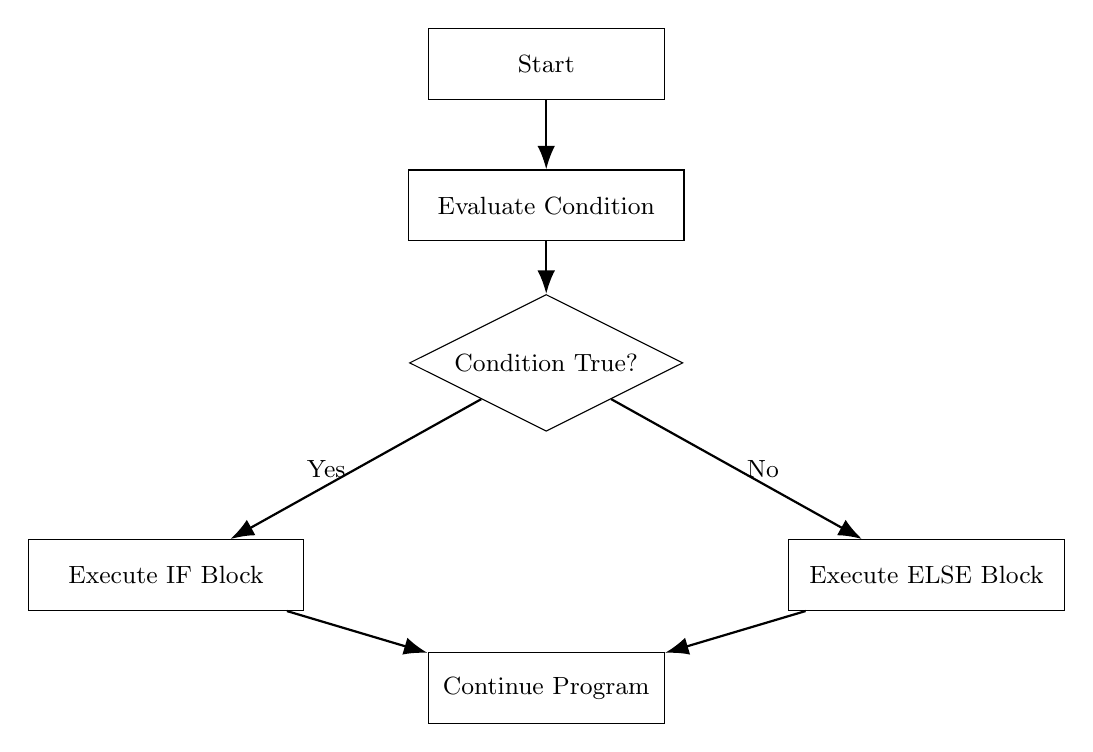
\begin{tikzpicture}[
node distance=1.8cm,
every node/.style={font=\small},
startstop/.style={
rectangle,draw,
minimum width=3cm,
minimum height=0.9cm},
process/.style={
rectangle,draw,
minimum width=3.5cm,
minimum height=0.9cm},
decision/.style={
diamond,draw,
aspect=2,
align=center},
arrow/.style={
-{Latex[length=3mm]},
thick}
]

\node(start)[startstop]{Start};

\node(input)[process,below of=start]{Evaluate Condition};

\node(decision)[decision,below of=input,yshift=-0.2cm]{Condition True?};

\node(trueblock)[process,below left=1.8cm and 2.2cm of decision]{Execute IF Block};

\node(falseblock)[process,below right=1.8cm and 2.2cm of decision]{Execute ELSE Block};

\node(end)[startstop,below=2.8cm of decision]{Continue Program};

\draw[arrow](start)--(input);
\draw[arrow](input)--(decision);

\draw[arrow](decision)--node[left]{Yes}(trueblock);
\draw[arrow](decision)--node[right]{No}(falseblock);

\draw[arrow](trueblock)--(end);
\draw[arrow](falseblock)--(end);

\end{tikzpicture}

\end{center}
\chapter{Functions}

\section{What is a Function?}

A function is a reusable block of code that performs a specific task.
Functions help organize programs, reduce code repetition, and improve readability.

For example, instead of writing the same code many times, you can place it inside a function and call it whenever needed.

Functions are one of the most important concepts in C programming because they make programs modular and easier to maintain.

\section{Why Use Functions?}

Functions provide many advantages in programming.

\begin{itemize}
    \item Reduce code duplication.
    \item Improve program readability.
    \item Make programs easier to maintain.
    \item Simplify debugging and testing.
    \item Allow code to be reused in different parts of a program.
\end{itemize}

Large software projects are typically divided into many small functions, each responsible for a specific task.

\section{Function Declaration (Prototype)}

Before a function is used, the compiler should know its name, return type, and parameters. This information is provided through a function declaration, also called a function prototype.

General syntax:

\begin{lstlisting}[language=C]
return_type function_name(parameter_list);
\end{lstlisting}

Example:

\begin{lstlisting}[language=C]
int add(int, int);
\end{lstlisting}

This declaration tells the compiler that a function named \texttt{add} exists, returns an integer, and accepts two integer parameters.

\section{Function Definition}

The function definition contains the actual code that performs the required task.

General syntax:

\begin{lstlisting}[language=C]
return_type function_name(parameters)
{
    /* Function body */
}
\end{lstlisting}

Example:

\begin{lstlisting}[language=C]
int add(int a, int b)
{
    return a + b;
}
\end{lstlisting}

In this example, the function receives two integers, adds them together, and returns the result.

\section{Function Call}

A function call transfers program control to the function so that it can perform its task.

Example:

\begin{lstlisting}[language=C]
#include <stdio.h>

int add(int, int);

int main(void)
{
    int result;

    result = add(10, 15);

    printf("Result = %d\n", result);

    return 0;
}

int add(int a, int b)
{
    return a + b;
}
\end{lstlisting}

Output:

\begin{lstlisting}
Result = 25
\end{lstlisting}

\section{How Function Calls Work}

The execution process is as follows:

\begin{enumerate}
    \item The program reaches the function call.
    \item Control is transferred to the function.
    \item The function executes its statements.
    \item A value may be returned.
    \item Control returns to the calling function.
\end{enumerate}
\section{Parameters and Arguments}

Functions often need data to perform their tasks. This data is passed through parameters and arguments.

An \textbf{argument} is the actual value passed to a function when it is called.

A \textbf{parameter} is the variable declared in the function definition that receives the value.

Example:

\begin{lstlisting}[language=C]
#include <stdio.h>

int multiply(int x, int y);

int main(void)
{
    int result;

    result = multiply(6, 8);

    printf("Result = %d\n", result);

    return 0;
}

int multiply(int x, int y)
{
    return x * y;
}
\end{lstlisting}

Output:

\begin{lstlisting}
Result = 48
\end{lstlisting}

In this example:

\begin{itemize}
    \item The values 6 and 8 are arguments.
    \item The variables x and y are parameters.
\end{itemize}

\section{Return Values}

Many functions return a value to the calling function.

The \texttt{return} statement terminates the function and sends a value back.

Example:

\begin{lstlisting}[language=C]
double square(double number)
{
    return number * number;
}
\end{lstlisting}

A function may return only one value directly.

\section{Void Functions}

Some functions perform an action but do not return a value.

These functions use the keyword \texttt{void}.

Example:

\begin{lstlisting}[language=C]
#include <stdio.h>

void displayMessage(void);

int main(void)
{
    displayMessage();

    return 0;
}

void displayMessage(void)
{
    printf("Welcome to C Programming!\n");
}
\end{lstlisting}

Output:

\begin{lstlisting}
Welcome to C Programming!
\end{lstlisting}

\section{Function Flow}

The following sequence describes how a function call is executed.

\begin{enumerate}
    \item The program executes statements in \texttt{main()}.
    \item A function is called.
    \item Arguments are copied to the function parameters.
    \item The function performs its task.
    \item The function returns a value (if any).
    \item Execution continues in the calling function.
\end{enumerate}

\section{Code Analysis}

Study the following example carefully.

\begin{lstlisting}[language=C]
#include <stdio.h>

int square(int number);

int main(void)
{
    int value = 7;

    printf("%d\n", square(value));

    return 0;
}

int square(int number)
{
    return number * number;
}
\end{lstlisting}

Output:

\begin{lstlisting}
49
\end{lstlisting}

Analysis:

\begin{itemize}
    \item The variable \texttt{value} stores the number 7.
    \item The function \texttt{square()} receives this value.
    \item The function multiplies the value by itself.
    \item The result (49) is returned to \texttt{main()}.
    \item The returned value is printed on the screen.
\end{itemize}

\section{Best Practices}

\begin{itemize}
    \item Give functions meaningful names.
    \item Keep each function focused on a single task.
    \item Avoid writing excessively long functions.
    \item Document complex functions with comments.
    \item Reuse existing functions whenever possible.
\end{itemize}
\section{Common Beginner Mistakes}

When learning functions, beginners often make the following mistakes:

\begin{itemize}
    \item Forgetting to declare a function before calling it.
    \item Using the wrong return type.
    \item Forgetting the \texttt{return} statement in non-\texttt{void} functions.
    \item Passing arguments with incorrect data types.
    \item Writing functions that perform too many unrelated tasks.
\end{itemize}

Understanding these mistakes early helps you write more reliable programs.

\section{Did You Know?}

Modern software systems may contain thousands of functions. Large applications divide complex tasks into many small, reusable functions, making development easier and improving code quality.

\section{Quick Quiz}

Choose the correct answer.

\begin{enumerate}
    \item Which keyword is used to return a value from a function?
    \begin{itemize}
        \item break
        \item return
        \item exit
        \item stop
    \end{itemize}

    \item Which keyword indicates that a function does not return a value?
    \begin{itemize}
        \item null
        \item empty
        \item void
        \item none
    \end{itemize}
\end{enumerate}

\section{Interview Questions}

These questions are frequently asked during programming interviews.

\begin{enumerate}
    \item What is the purpose of a function?
    \item What is the difference between a function declaration and a function definition?
    \item Explain the difference between parameters and arguments.
    \item Why are functions important in modular programming?
    \item What happens when a function returns a value?
\end{enumerate}

\section{Key Terms}

\begin{itemize}
    \item Function
    \item Function Prototype
    \item Function Definition
    \item Function Call
    \item Parameter
    \item Argument
    \item Return Value
    \item Void Function
    \item Modular Programming
\end{itemize}

\section{Chapter Summary}

In this chapter, you learned how functions divide large programs into smaller, reusable units. You explored function declarations, definitions, function calls, parameters, arguments, return values, and \texttt{void} functions. Writing well-designed functions improves readability, maintainability, and software quality.

\section{Programming Exercises}

\subsection*{Easy}

\begin{enumerate}
    \item Write a function that returns the square of an integer.
    \item Write a function that prints a welcome message.
    \item Write a function that calculates the sum of two integers.
\end{enumerate}

\subsection*{Intermediate}

\begin{enumerate}
    \item Write a function that determines whether a number is even or odd.
    \item Create a function that returns the larger of two numbers.
    \item Write a function that calculates the area of a rectangle.
\end{enumerate}

\subsection*{Advanced}

\begin{enumerate}
    \item Build a calculator using separate functions for each operation.
    \item Write a function that calculates the factorial of a number.
    \item Develop a menu-driven application that uses multiple functions.
\end{enumerate}

\section{Mini Project}

Create a Student Management Program.

The program should contain separate functions to:

\begin{itemize}
    \item Read student information.
    \item Calculate the average score.
    \item Determine whether the student passed.
    \item Display a formatted report.
\end{itemize}

\section{Challenge Project}

Develop a Banking Application.

The program should contain separate functions for:

\begin{itemize}
    \item Deposit
    \item Withdrawal
    \item Balance Inquiry
    \item Display Menu
\end{itemize}

Use functions to organize the program into small, reusable components.

\section{Looking Ahead}

In the next chapter, you will learn about arrays. Arrays allow programs to store multiple values of the same data type using a single variable name, making it much easier to process collections of data efficiently.
\chapter{Arrays}

\section{Chapter Overview}

In previous chapters, each variable stored only one value. However, many programming problems require storing a collection of values, such as students' grades, temperatures, or monthly sales.

Arrays provide an efficient way to store multiple values of the same data type using a single variable name.

This chapter introduces arrays, explains how they are stored in memory, and demonstrates how to access and manipulate their elements.

\section{Learning Objectives}

After completing this chapter, you will be able to:

\begin{itemize}
    \item Understand the concept of arrays.
    \item Declare and initialize arrays.
    \item Access individual array elements.
    \item Modify array values.
    \item Traverse arrays using loops.
    \item Apply arrays to solve real-world programming problems.
\end{itemize}

\section{Real-World Scenario}

Imagine a teacher who wants to store the grades of 30 students.

Without arrays, the program would require 30 separate variables:

\begin{lstlisting}[language=C]
int grade1;
int grade2;
int grade3;
/* ... */
int grade30;
\end{lstlisting}

Managing such code is difficult and error-prone.

With an array, all grades can be stored using a single variable:

\begin{lstlisting}[language=C]
int grades[30];
\end{lstlisting}

This approach is simpler, cleaner, and much easier to maintain.

\section{What Is an Array?}

An array is a collection of elements that all have the same data type.

Each element occupies a consecutive location in memory and is identified by its index.

The first element always has index 0.

For example, an array containing five integers has the following indices:

\begin{center}
\begin{tabular}{|c|c|c|c|c|}
\hline
0 & 1 & 2 & 3 & 4 \\
\hline
\end{tabular}
\end{center}

Understanding array indexing is one of the most important concepts in C programming.
\section{Declaring an Array}

General syntax:

\begin{lstlisting}[language=C]
data_type array_name[size];
\end{lstlisting}

Example:

\begin{lstlisting}[language=C]
int numbers[5];
float temperatures[7];
char name[20];
\end{lstlisting}

The number inside the brackets specifies how many elements the array can store.

\section{Array Initialization}

Arrays may be initialized when they are declared.

Example:

\begin{lstlisting}[language=C]
int numbers[5] = {10, 20, 30, 40, 50};
\end{lstlisting}

Another valid form is:

\begin{lstlisting}[language=C]
int numbers[] = {10, 20, 30, 40, 50};
\end{lstlisting}

In this case, the compiler automatically determines the array size.

\section{Accessing Array Elements}

Each element is accessed using its index.

Example:

\begin{lstlisting}[language=C]
#include <stdio.h>

int main(void)
{
    int numbers[5] = {10,20,30,40,50};

    printf("%d\n", numbers[0]);
    printf("%d\n", numbers[3]);

    return 0;
}
\end{lstlisting}

Output:

\begin{lstlisting}
10
40
\end{lstlisting}

Remember that array indexing always starts at zero.
\section{Modifying Array Elements}

Array elements can be modified by assigning new values to their indices.

Example:

\begin{lstlisting}[language=C]
#include <stdio.h>

int main(void)
{
    int numbers[5] = {10, 20, 30, 40, 50};

    numbers[2] = 100;

    printf("%d\n", numbers[2]);

    return 0;
}
\end{lstlisting}

Output:

\begin{lstlisting}
100
\end{lstlisting}

Changing one element does not affect the other elements in the array.

\section{Traversing an Array}

One of the greatest advantages of arrays is that all elements can be processed using loops.

Example:

\begin{lstlisting}[language=C]
#include <stdio.h>

int main(void)
{
    int numbers[5] = {10, 20, 30, 40, 50};
    int i;

    for(i = 0; i < 5; i++)
    {
        printf("%d\n", numbers[i]);
    }

    return 0;
}
\end{lstlisting}

Output:

\begin{lstlisting}
10
20
30
40
50
\end{lstlisting}

The loop variable starts at index 0 and continues until the last valid index.

\section{Reading Array Values from the User}

The \texttt{scanf()} function can be combined with loops to fill an array.

Example:

\begin{lstlisting}[language=C]
#include <stdio.h>

int main(void)
{
    int numbers[5];
    int i;

    printf("Enter five integers:\n");

    for(i = 0; i < 5; i++)
    {
        scanf("%d", &numbers[i]);
    }

    printf("\nYou entered:\n");

    for(i = 0; i < 5; i++)
    {
        printf("%d ", numbers[i]);
    }

    return 0;
}
\end{lstlisting}

\section{Memory Layout of an Array}

Array elements are stored in consecutive memory locations.

Example:

\begin{center}
\begin{tabular}{|c|c|c|c|c|}
\hline
Index & 0 & 1 & 2 & 3 \\
\hline
Value & 15 & 28 & 42 & 60 \\
\hline
\end{tabular}
\end{center}

Although the elements appear as a single variable, each element occupies its own memory location.

\section{Code Analysis}

Study the following program.

\begin{lstlisting}[language=C]
#include <stdio.h>

int main(void)
{
    int marks[4] = {80, 75, 92, 88};
    int i;

    for(i = 0; i < 4; i++)
    {
        printf("%d\n", marks[i]);
    }

    return 0;
}
\end{lstlisting}

Analysis:

\begin{itemize}
    \item An array named \texttt{marks} stores four integer values.
    \item The variable \texttt{i} is used as the loop counter.
    \item Each iteration prints one array element.
    \item The loop stops after printing the last element.
\end{itemize}

\section{Best Practices}

\begin{itemize}
    \item Use meaningful names for arrays.
    \item Never access an index outside the array bounds.
    \item Initialize arrays whenever possible.
    \item Use loops to process array elements.
    \item Keep the array size consistent with the number of stored elements.
\end{itemize}
\section{Common Beginner Mistakes}

Working with arrays can be challenging for beginners. The following mistakes are very common:

\begin{itemize}
    \item Forgetting that array indexing starts at 0.
    \item Accessing elements outside the array bounds.
    \item Declaring an array that is too small.
    \item Using an incorrect loop condition.
    \item Forgetting to initialize array elements before using them.
\end{itemize}

Always ensure that array indices remain within the valid range.

\section{Introduction to Multidimensional Arrays}

A multidimensional array is an array whose elements are themselves arrays.

The most common multidimensional array is the two-dimensional array.

General syntax:

\begin{lstlisting}[language=C]
int matrix[3][4];
\end{lstlisting}

This declaration creates a table with three rows and four columns.

Example:

\begin{lstlisting}[language=C]
int matrix[2][3] =
{
    {1, 2, 3},
    {4, 5, 6}
};
\end{lstlisting}

Multidimensional arrays will be discussed in greater detail in a later chapter.

\section{Did You Know?}

Arrays are widely used in computer science to represent tables, matrices, images, game boards, and many other data structures. Understanding arrays is essential before learning pointers and dynamic memory allocation.

\section{Quick Quiz}

Choose the correct answer.

\begin{enumerate}
    \item What is the index of the first element in an array?
    \begin{itemize}
        \item 0
        \item 1
        \item -1
        \item It depends on the compiler.
    \end{itemize}

    \item Which statement correctly declares an array of 10 integers?
    \begin{itemize}
        \item int numbers;
        \item int numbers(10);
        \item int numbers[10];
        \item array numbers[10];
    \end{itemize}
\end{enumerate}

\section{Key Terms}

\begin{itemize}
    \item Array
    \item Element
    \item Index
    \item Array Traversal
    \item Initialization
    \item Multidimensional Array
\end{itemize}

\section{Chapter Summary}

In this chapter, you learned how arrays store multiple values of the same data type. You practiced declaring, initializing, accessing, modifying, and traversing arrays using loops. You also learned about common mistakes and received an introduction to multidimensional arrays.

\section{Programming Exercises}

\subsection*{Easy}

\begin{enumerate}
    \item Store five integers in an array and display them.
    \item Read ten integers from the user and print them.
    \item Calculate the sum of all elements in an array.
\end{enumerate}

\subsection*{Intermediate}

\begin{enumerate}
    \item Find the largest value in an array.
    \item Find the smallest value in an array.
    \item Calculate the average of array elements.
\end{enumerate}

\subsection*{Advanced}

\begin{enumerate}
    \item Reverse the elements of an array.
    \item Sort an array in ascending order.
    \item Search for a specific value entered by the user.
\end{enumerate}

\section{Mini Project}

Create a Student Grades Analyzer.

The program should:

\begin{itemize}
    \item Read the grades of ten students.
    \item Calculate the average grade.
    \item Find the highest grade.
    \item Find the lowest grade.
    \item Display a formatted report.
\end{itemize}

\section{Challenge Project}

Develop a Statistics Program.

The program should:

\begin{itemize}
    \item Read twenty numbers.
    \item Compute the sum.
    \item Compute the average.
    \item Find the maximum value.
    \item Find the minimum value.
    \item Display all results clearly.
\end{itemize}

\section{Looking Ahead}

In the next chapter, you will learn about strings in C. Strings are arrays of characters and are used extensively for storing and manipulating text.
\chapter{Strings}

\section{Chapter Overview}

Text processing is an essential part of programming. Applications such as text editors, web browsers, search engines, and databases all work with textual data.

In C, a string is represented as an array of characters terminated by a special null character. Understanding strings is essential for developing real-world applications.

\section{Learning Objectives}

After completing this chapter, you will be able to:

\begin{itemize}
    \item Understand what a string is.
    \item Declare and initialize strings.
    \item Read and display strings.
    \item Access individual characters.
    \item Understand the null character.
    \item Process strings using loops.
\end{itemize}

\section{Real-World Scenario}

Suppose you are creating a student management system.

Instead of storing only numbers, you also need to store each student's name.

A string allows you to store an entire word or sentence using a single variable.

For example:

\begin{lstlisting}[language=C]
char name[30];
\end{lstlisting}

This variable can store up to 29 visible characters plus the terminating null character.

\section{What Is a String?}

A string is a sequence of characters stored inside a character array.

Unlike ordinary character arrays, a string always ends with the special character:

\begin{lstlisting}[language=C]
'\0'
\end{lstlisting}

This character is called the \textbf{null terminator}.

It tells the compiler where the string ends.

Example:

\begin{lstlisting}[language=C]
char word[] = "Hello";
\end{lstlisting}

Internally, the string is stored as:

\begin{center}
\begin{tabular}{|c|c|c|c|c|c|}
\hline
H & e & l & l & o & \textbackslash0 \\
\hline
\end{tabular}
\end{center}

The null character is stored automatically by the compiler.
\section{Declaring Strings}

General syntax:

\begin{lstlisting}[language=C]
char string_name[size];
\end{lstlisting}

Examples:

\begin{lstlisting}[language=C]
char firstName[20];
char lastName[30];
char country[25];
\end{lstlisting}

Each element of the array stores one character.

\section{Initializing Strings}

Strings can be initialized in several ways.

Method 1:

\begin{lstlisting}[language=C]
char city[] = "London";
\end{lstlisting}

Method 2:

\begin{lstlisting}[language=C]
char city[20] = "London";
\end{lstlisting}

Method 3:

\begin{lstlisting}[language=C]
char city[] =
{'L','o','n','d','o','n','\0'};
\end{lstlisting}

The first method is the most common and easiest to read.

\section{Displaying Strings}

The \texttt{printf()} function displays strings using the \texttt{\%s} format specifier.

Example:

\begin{lstlisting}[language=C]
#include <stdio.h>

int main(void)
{
    char language[] = "C Programming";

    printf("%s\n", language);

    return 0;
}
\end{lstlisting}

Output:

\begin{lstlisting}
C Programming
\end{lstlisting}

\section{Accessing Individual Characters}

Since a string is an array, each character has its own index.

Example:

\begin{lstlisting}[language=C]
char word[] = "Programming";

printf("%c\n", word[0]);
printf("%c\n", word[4]);
\end{lstlisting}

Output:

\begin{lstlisting}
P
r
\end{lstlisting}

Remember that indexing always begins with zero.
\section{Reading Strings}

The C language provides several ways to read strings from the user.

The safest and most recommended function is \texttt{fgets()} because it helps prevent buffer overflow.

General syntax:

\begin{lstlisting}[language=C]
fgets(string, size, stdin);
\end{lstlisting}

Example:

\begin{lstlisting}[language=C]
#include <stdio.h>

int main(void)
{
    char name[30];

    printf("Enter your name: ");
    fgets(name, sizeof(name), stdin);

    printf("Hello, %s", name);

    return 0;
}
\end{lstlisting}

Sample Output:

\begin{lstlisting}
Enter your name: Alice
Hello, Alice
\end{lstlisting}

\section{Why \texttt{fgets()} Is Preferred}

Older C programs often used the \texttt{gets()} function.

However, \texttt{gets()} does not check the size of the destination array, making it unsafe.

For this reason, \texttt{gets()} was removed from the C Standard Library.

Modern C programs should use \texttt{fgets()} whenever possible.

\section{Traversing a String}

Since a string is an array of characters, loops can be used to process each character individually.

Example:

\begin{lstlisting}[language=C]
#include <stdio.h>

int main(void)
{
    char word[] = "Computer";
    int i = 0;

    while(word[i] != '\0')
    {
        printf("%c\n", word[i]);
        i++;
    }

    return 0;
}
\end{lstlisting}

Output:

\begin{lstlisting}
C
o
m
p
u
t
e
r
\end{lstlisting}

The loop stops when it reaches the null character.

\section{The \texttt{string.h} Library}

The header file \texttt{string.h} provides many useful functions for working with strings.

To use these functions, include:

\begin{lstlisting}[language=C]
#include <string.h>
\end{lstlisting}

Some of the most frequently used string functions are:

\begin{center}
\begin{tabular}{|l|l|}
\hline
Function & Purpose \\
\hline
strlen() & Returns the length of a string \\
strcpy() & Copies one string to another \\
strcat() & Concatenates two strings \\
strcmp() & Compares two strings \\
\hline
\end{tabular}
\end{center}

These functions simplify many common string operations.
\section{The \texttt{strlen()} Function}

The \texttt{strlen()} function returns the number of characters in a string, excluding the null terminator.

Example:

\begin{lstlisting}[language=C]
#include <stdio.h>
#include <string.h>

int main(void)
{
    char text[] = "Programming";

    printf("%zu\n", strlen(text));

    return 0;
}
\end{lstlisting}

Output:

\begin{lstlisting}
11
\end{lstlisting}

\section{The \texttt{strcpy()} Function}

The \texttt{strcpy()} function copies one string into another.

Example:

\begin{lstlisting}[language=C]
#include <stdio.h>
#include <string.h>

int main(void)
{
    char source[] = "C Language";
    char destination[30];

    strcpy(destination, source);

    printf("%s\n", destination);

    return 0;
}
\end{lstlisting}

\section{The \texttt{strcat()} Function}

The \texttt{strcat()} function appends one string to another.

Example:

\begin{lstlisting}[language=C]
#include <stdio.h>
#include <string.h>

int main(void)
{
    char first[30] = "Hello ";
    char second[] = "World";

    strcat(first, second);

    printf("%s\n", first);

    return 0;
}
\end{lstlisting}

Output:

\begin{lstlisting}
Hello World
\end{lstlisting}

\section{The \texttt{strcmp()} Function}

The \texttt{strcmp()} function compares two strings.

Example:

\begin{lstlisting}[language=C]
#include <stdio.h>
#include <string.h>

int main(void)
{
    char first[] = "Apple";
    char second[] = "Apple";

    if(strcmp(first, second) == 0)
    {
        printf("The strings are equal.\n");
    }

    return 0;
}
\end{lstlisting}

Output:

\begin{lstlisting}
The strings are equal.
\end{lstlisting}
\section{Code Analysis}

Study the following program carefully.

\begin{lstlisting}[language=C]
#include <stdio.h>
#include <string.h>

int main(void)
{
    char firstName[20] = "John";
    char lastName[20] = "Smith";
    char fullName[50];

    strcpy(fullName, firstName);
    strcat(fullName, " ");
    strcat(fullName, lastName);

    printf("%s\n", fullName);

    return 0;
}
\end{lstlisting}

Output:

\begin{lstlisting}
John Smith
\end{lstlisting}

Analysis:

\begin{itemize}
    \item The program creates three character arrays.
    \item \texttt{strcpy()} copies the first name into \texttt{fullName}.
    \item \texttt{strcat()} appends a space.
    \item Another call to \texttt{strcat()} appends the last name.
    \item The completed string is displayed.
\end{itemize}

\section{Common Beginner Mistakes}

Many beginners make the following mistakes when working with strings:

\begin{itemize}
    \item Forgetting the null terminator.
    \item Declaring arrays that are too small.
    \item Using \texttt{==} instead of \texttt{strcmp()} to compare strings.
    \item Forgetting to include \texttt{string.h}.
    \item Accessing characters outside the string bounds.
\end{itemize}

Avoiding these mistakes will make your programs more reliable.

\section{Best Practices}

\begin{itemize}
    \item Prefer \texttt{fgets()} over unsafe input functions.
    \item Allocate enough space for the null terminator.
    \item Always check array sizes before copying strings.
    \item Use descriptive variable names.
    \item Include \texttt{string.h} when using string functions.
\end{itemize}

\section{Quick Quiz}

Choose the correct answer.

\begin{enumerate}
    \item Which function returns the length of a string?
    \begin{itemize}
        \item strcpy()
        \item strlen()
        \item strcmp()
        \item strcat()
    \end{itemize}

    \item Which function compares two strings?
    \begin{itemize}
        \item strcmp()
        \item strcat()
        \item strlen()
        \item scanf()
    \end{itemize}

    \item Which character marks the end of a string?
    \begin{itemize}
        \item '\n'
        \item '\t'
        \item '\0'
        \item ' '
    \end{itemize}
\end{enumerate}

\section{Key Terms}

\begin{itemize}
    \item String
    \item Character Array
    \item Null Terminator
    \item fgets()
    \item strlen()
    \item strcpy()
    \item strcat()
    \item strcmp()
\end{itemize}

\section{Chapter Summary}

In this chapter, you learned that strings in C are character arrays terminated by a null character. You practiced declaring, initializing, reading, displaying, and processing strings. You also learned to use the most important functions provided by the \texttt{string.h} library.

\section{Programming Exercises}

\subsection*{Easy}

\begin{enumerate}
    \item Read a name and display it.
    \item Display each character of a string on a separate line.
    \item Calculate the length of a string using \texttt{strlen()}.
\end{enumerate}

\subsection*{Intermediate}

\begin{enumerate}
    \item Copy one string into another.
    \item Concatenate two strings entered by the user.
    \item Compare two strings and indicate whether they are equal.
\end{enumerate}

\subsection*{Advanced}

\begin{enumerate}
    \item Count the number of vowels in a string.
    \item Reverse a string without using library functions.
    \item Determine whether a string is a palindrome.
\end{enumerate}

\section{Mini Project}

Create a Contact Manager.

The program should:

\begin{itemize}
    \item Read a person's name.
    \item Read a phone number.
    \item Display the stored information clearly.
\end{itemize}

\section{Challenge Project}

Develop a Text Analyzer.

The program should:

\begin{itemize}
    \item Read a sentence.
    \item Count letters.
    \item Count words.
    \item Count vowels.
    \item Count digits.
    \item Display a complete report.
\end{itemize}

\section{Looking Ahead}

In the next chapter, you will learn about pointers. Pointers are one of the most powerful features of C and provide direct access to memory addresses.
\chapter{Pointers}

\section{Chapter Overview}

Pointers are one of the most powerful features of the C programming language. They allow programs to work directly with memory addresses, making it possible to write efficient software, manipulate arrays, create dynamic data structures, and pass data efficiently between functions.

Although pointers may seem difficult at first, they become much easier once you understand how memory is organized.

\section{Learning Objectives}

After completing this chapter, you will be able to:

\begin{itemize}
    \item Understand what a pointer is.
    \item Declare pointer variables.
    \item Store memory addresses.
    \item Use the address operator.
    \item Use the dereference operator.
    \item Explain the relationship between pointers and variables.
\end{itemize}

\section{What Is a Pointer?}

A pointer is a variable that stores the memory address of another variable.

Unlike ordinary variables, which store values, pointers store locations in memory.

For example:

\begin{lstlisting}[language=C]
int number = 50;
\end{lstlisting}

The variable stores the value 50 somewhere in memory.

A pointer stores the address of that memory location.

\section{Memory and Variables}

Whenever a variable is declared, the operating system reserves a location in memory for it.

Example:

\begin{lstlisting}[language=C]
int age = 25;
\end{lstlisting}

Suppose the variable is stored at address:

\begin{lstlisting}
0x7FFE42A0
\end{lstlisting}

The value is:

\begin{lstlisting}
25
\end{lstlisting}

The exact address changes every time the program runs.

\section{The Address Operator (\texttt{\&})}

The address operator returns the memory address of a variable.

Example:

\begin{lstlisting}[language=C]
#include <stdio.h>

int main(void)
{
    int number = 100;

    printf("%p\n", (void *)&number);

    return 0;
}
\end{lstlisting}

Output:

\begin{lstlisting}
0x7FFE42A0
\end{lstlisting}

The printed address will be different on each computer and each execution.
\section{Declaring Pointer Variables}

General syntax:

\begin{lstlisting}[language=C]
data_type *pointer_name;
\end{lstlisting}

Examples:

\begin{lstlisting}[language=C]
int *p;
float *temperature;
char *letter;
\end{lstlisting}

The asterisk indicates that the variable is a pointer.

\section{Assigning an Address to a Pointer}

A pointer stores an address using the address operator.

Example:

\begin{lstlisting}[language=C]
#include <stdio.h>

int main(void)
{
    int number = 25;
    int *ptr;

    ptr = &number;

    printf("%p\n", (void *)ptr);

    return 0;
}
\end{lstlisting}

Now the pointer stores the address of the variable \texttt{number}.

\section{The Dereference Operator (\texttt{*})}

The dereference operator accesses the value stored at the address contained in a pointer.

Example:

\begin{lstlisting}[language=C]
#include <stdio.h>

int main(void)
{
    int number = 25;
    int *ptr = &number;

    printf("%d\n", *ptr);

    return 0;
}
\end{lstlisting}

Output:

\begin{lstlisting}
25
\end{lstlisting}

The expression \texttt{*ptr} means:

"Go to the memory address stored in \texttt{ptr} and retrieve the value."
\section{Pointers and Variables}

A pointer and the variable it points to are closely related.

Consider the following example:

\begin{lstlisting}[language=C]
#include <stdio.h>

int main(void)
{
    int number = 50;
    int *ptr = &number;

    printf("Value of number: %d\n", number);
    printf("Address of number: %p\n", (void *)&number);
    printf("Value stored in ptr: %p\n", (void *)ptr);
    printf("Value pointed to by ptr: %d\n", *ptr);

    return 0;
}
\end{lstlisting}

Sample Output:

\begin{lstlisting}
Value of number: 50
Address of number: 0x7FFE42A0
Value stored in ptr: 0x7FFE42A0
Value pointed to by ptr: 50
\end{lstlisting}

Notice that the pointer stores the memory address, while the dereference operator retrieves the value stored at that address.

\section{Changing Values Through a Pointer}

Pointers can modify the value of the variable they point to.

Example:

\begin{lstlisting}[language=C]
#include <stdio.h>

int main(void)
{
    int number = 10;
    int *ptr = &number;

    *ptr = 100;

    printf("%d\n", number);

    return 0;
}
\end{lstlisting}

Output:

\begin{lstlisting}
100
\end{lstlisting}

Changing the value through the pointer also changes the original variable because both refer to the same memory location.

\section{NULL Pointers}

Sometimes a pointer should not point to any valid memory location.

Such pointers are initialized with the constant \texttt{NULL}.

Example:

\begin{lstlisting}[language=C]
#include <stdio.h>

int main(void)
{
    int *ptr = NULL;

    if(ptr == NULL)
    {
        printf("Pointer is NULL.\n");
    }

    return 0;
}
\end{lstlisting}

Initializing pointers to \texttt{NULL} helps prevent accidental access to invalid memory.

\section{Pointers and Arrays}

The name of an array represents the address of its first element.

Example:

\begin{lstlisting}[language=C]
#include <stdio.h>

int main(void)
{
    int numbers[5] = {10,20,30,40,50};

    printf("%d\n", *numbers);
    printf("%d\n", *(numbers + 1));
    printf("%d\n", *(numbers + 2));

    return 0;
}
\end{lstlisting}

Output:

\begin{lstlisting}
10
20
30
\end{lstlisting}

This demonstrates the close relationship between arrays and pointers in C.

\section{Code Analysis}

Consider the following program.

\begin{lstlisting}[language=C]
#include <stdio.h>

int main(void)
{
    int value = 25;
    int *ptr = &value;

    printf("%d\n", *ptr);

    *ptr = 75;

    printf("%d\n", value);

    return 0;
}
\end{lstlisting}

Output:

\begin{lstlisting}
25
75
\end{lstlisting}

Analysis:

\begin{itemize}
    \item The pointer stores the address of \texttt{value}.
    \item The first \texttt{printf()} displays the original value.
    \item The assignment \texttt{*ptr = 75;} changes the value stored at that address.
    \item The second \texttt{printf()} confirms that the original variable has changed.
\end{itemize}

\section{Best Practices}

\begin{itemize}
    \item Always initialize pointers before using them.
    \item Use \texttt{NULL} for pointers that do not yet reference valid memory.
    \item Never dereference an uninitialized pointer.
    \item Use meaningful pointer names.
    \item Keep pointer operations as simple and readable as possible.
\end{itemize}
\section{Pointer Arithmetic}

Pointer arithmetic allows a pointer to move between elements of an array.

When an integer pointer is incremented, it moves to the next integer in memory.

Example:

\begin{lstlisting}[language=C]
#include <stdio.h>

int main(void)
{
    int numbers[3] = {10, 20, 30};
    int *ptr = numbers;

    printf("%d\n", *ptr);

    ptr++;

    printf("%d\n", *ptr);

    return 0;
}
\end{lstlisting}

Output:

\begin{lstlisting}
10
20
\end{lstlisting}

The pointer automatically advances by the size of one integer.

\section{Common Beginner Mistakes}

Pointers are powerful, but they require careful use.

Common mistakes include:

\begin{itemize}
    \item Dereferencing an uninitialized pointer.
    \item Forgetting to initialize pointers with valid addresses.
    \item Confusing the \texttt{*} and \texttt{\&} operators.
    \item Accessing memory outside an array.
    \item Forgetting to check for \texttt{NULL} before dereferencing.
\end{itemize}

Understanding these mistakes will help prevent program crashes and undefined behavior.

\section{Debugging Tips}

When debugging pointer-related programs:

\begin{itemize}
    \item Print pointer addresses using \texttt{\%p}.
    \item Verify that pointers are not \texttt{NULL}.
    \item Check array boundaries carefully.
    \item Initialize every pointer before using it.
    \item Change one thing at a time while debugging.
\end{itemize}

\section{Quick Quiz}

Choose the correct answer.

\begin{enumerate}
    \item What does a pointer store?
    \begin{itemize}
        \item A character
        \item A memory address
        \item An array
        \item A function
    \end{itemize}

    \item Which operator returns the address of a variable?
    \begin{itemize}
        \item *
        \item %
        \item &
        \item @
    \end{itemize}

    \item Which operator accesses the value stored at a pointer's address?
    \begin{itemize}
        \item *
        \item &
        \item %
        \item #
    \end{itemize}
\end{enumerate}

\section{Key Terms}

\begin{itemize}
    \item Pointer
    \item Address
    \item Dereference
    \item Address Operator
    \item NULL Pointer
    \item Pointer Arithmetic
\end{itemize}

\section{Chapter Summary}

In this chapter, you learned that pointers store memory addresses rather than ordinary values. You explored the address operator, the dereference operator, pointer variables, NULL pointers, pointer arithmetic, and the relationship between pointers and arrays. These concepts form the foundation for dynamic memory management and advanced programming in C.

\section{Programming Exercises}

\subsection*{Easy}

\begin{enumerate}
    \item Declare a pointer to an integer.
    \item Print the address of a variable.
    \item Display a value using a pointer.
\end{enumerate}

\subsection*{Intermediate}

\begin{enumerate}
    \item Modify a variable through a pointer.
    \item Traverse an array using pointer arithmetic.
    \item Compare array indexing with pointer notation.
\end{enumerate}

\subsection*{Advanced}

\begin{enumerate}
    \item Swap two variables using pointers.
    \item Write a function that receives a pointer as a parameter.
    \item Reverse an array using pointers.
\end{enumerate}

\section{Mini Project}

Create a Pointer Demonstration Program.

The program should:

\begin{itemize}
    \item Declare variables.
    \item Display their addresses.
    \item Modify values using pointers.
    \item Display the updated values.
\end{itemize}

\section{Challenge Project}

Develop a Dynamic Statistics Program.

The program should:

\begin{itemize}
    \item Read an array of integers.
    \item Process the array using only pointer arithmetic.
    \item Calculate the sum.
    \item Calculate the average.
    \item Display the maximum and minimum values.
\end{itemize}

\section{Looking Ahead}

In the next chapter, you will learn about structures. Structures allow programmers to group related variables of different data types into a single user-defined data type.
\chapter{Structures}

\section{Chapter Overview}

In previous chapters, each variable stored a single value of one data type. However, many real-world objects contain different types of information.

For example, a student has a name, an ID number, an age, and a grade. Storing these values in separate variables becomes difficult as programs grow.

Structures allow programmers to group related data into a single user-defined data type.

\section{Learning Objectives}

After completing this chapter, you will be able to:

\begin{itemize}
    \item Understand the purpose of structures.
    \item Declare structure types.
    \item Create structure variables.
    \item Access structure members.
    \item Initialize structures.
    \item Pass structures to functions.
\end{itemize}

\section{Real-World Scenario}

Suppose you are developing a student management system.

Each student has:

\begin{itemize}
    \item Student ID
    \item Name
    \item Age
    \item GPA
\end{itemize}

Instead of storing these values in separate variables, a structure groups them together.

\section{What Is a Structure?}

A structure is a user-defined data type that groups variables of different data types under one name.

General syntax:

\begin{lstlisting}[language=C]
struct StructureName
{
    data_type member1;
    data_type member2;
    data_type member3;
};
\end{lstlisting}

Unlike arrays, structure members may have different data types.
\section{Declaring a Structure}

Example:

\begin{lstlisting}[language=C]
struct Student
{
    int id;
    char name[30];
    int age;
    float gpa;
};
\end{lstlisting}

This declaration creates a new data type named \texttt{Student}.

No memory is allocated until a variable is created.

\section{Creating Structure Variables}

Example:

\begin{lstlisting}[language=C]
struct Student student1;
\end{lstlisting}

Now memory is allocated for all members of the structure.

\section{Accessing Structure Members}

The dot operator (\texttt{.}) is used to access members.

Example:

\begin{lstlisting}[language=C]
student1.id = 1001;
student1.age = 20;
student1.gpa = 3.85;
\end{lstlisting}

For character arrays:

\begin{lstlisting}[language=C]
strcpy(student1.name, "Alice");
\end{lstlisting}

Remember to include:

\begin{lstlisting}[language=C]
#include <string.h>
\end{lstlisting}

when using \texttt{strcpy()}.

\section{Complete Example}

\begin{lstlisting}[language=C]
#include <stdio.h>
#include <string.h>

struct Student
{
    int id;
    char name[30];
    int age;
    float gpa;
};

int main(void)
{
    struct Student student1;

    student1.id = 1001;
    student1.age = 20;
    student1.gpa = 3.75;

    strcpy(student1.name, "Alice");

    printf("ID: %d\n", student1.id);
    printf("Name: %s\n", student1.name);
    printf("Age: %d\n", student1.age);
    printf("GPA: %.2f\n", student1.gpa);

    return 0;
}
\end{lstlisting}

Output:

\begin{lstlisting}
ID: 1001
Name: Alice
Age: 20
GPA: 3.75
\end{lstlisting}
\section{Initializing Structures}

Structure variables can be initialized when they are declared.

Example:

\begin{lstlisting}[language=C]
struct Student student1 = {1001, "Alice", 20, 3.75};
\end{lstlisting}

Each value is assigned to the corresponding structure member in the order they are declared.

\section{Arrays of Structures}

Programs often need to store multiple records. An array of structures makes this possible.

Example:

\begin{lstlisting}[language=C]
struct Student students[3];
\end{lstlisting}

Each element of the array is a complete structure.

Example:

\begin{lstlisting}[language=C]
students[0].id = 1001;
students[1].id = 1002;
students[2].id = 1003;
\end{lstlisting}

Arrays of structures are widely used in database and management applications.

\section{Nested Structures}

A structure can contain another structure as one of its members.

Example:

\begin{lstlisting}[language=C]
struct Date
{
    int day;
    int month;
    int year;
};

struct Student
{
    char name[30];
    struct Date birthday;
};
\end{lstlisting}

Accessing nested members:

\begin{lstlisting}[language=C]
student1.birthday.day = 15;
student1.birthday.month = 6;
student1.birthday.year = 2005;
\end{lstlisting}

Nested structures help organize related information clearly.

\section{Structures and Functions}

Structures can be passed to functions just like ordinary variables.

Example:

\begin{lstlisting}[language=C]
#include <stdio.h>

struct Student
{
    int id;
    float gpa;
};

void displayStudent(struct Student s)
{
    printf("ID: %d\n", s.id);
    printf("GPA: %.2f\n", s.gpa);
}

int main(void)
{
    struct Student student = {1001, 3.80};

    displayStudent(student);

    return 0;
}
\end{lstlisting}

Passing structures to functions improves program organization and modularity.

\section{The \texttt{typedef} Keyword}

The \texttt{typedef} keyword creates an alias for a data type.

Example:

\begin{lstlisting}[language=C]
typedef struct
{
    int id;
    char name[30];
} Student;
\end{lstlisting}

Now variables can be declared more simply:

\begin{lstlisting}[language=C]
Student student1;
\end{lstlisting}

Using \texttt{typedef} makes programs easier to read.
\section{Code Analysis}

Study the following example.

\begin{lstlisting}[language=C]
#include <stdio.h>

typedef struct
{
    int id;
    char grade;
} Student;

int main(void)
{
    Student s = {101, 'A'};

    printf("%d\n", s.id);
    printf("%c\n", s.grade);

    return 0;
}
\end{lstlisting}

Output:

\begin{lstlisting}
101
A
\end{lstlisting}

Analysis:

\begin{itemize}
    \item A new type named \texttt{Student} is created using \texttt{typedef}.
    \item A variable named \texttt{s} is initialized.
    \item The dot operator accesses the members.
    \item The values are displayed using \texttt{printf()}.
\end{itemize}

\section{Best Practices}

\begin{itemize}
    \item Group logically related data into structures.
    \item Use meaningful member names.
    \item Prefer \texttt{typedef} for cleaner code.
    \item Keep structures focused on a single concept.
    \item Pass large structures by pointer for better performance.
\end{itemize}
\section{Common Beginner Mistakes}

Many beginners encounter the following problems when using structures:

\begin{itemize}
    \item Forgetting to declare a structure variable.
    \item Using the dot operator with a structure pointer instead of the arrow operator.
    \item Forgetting to include \texttt{string.h} when using \texttt{strcpy()}.
    \item Declaring members with inappropriate data types.
    \item Forgetting to initialize structure members before using them.
\end{itemize}

Carefully designing structures improves program organization and reduces errors.

\section{Debugging Tips}

When debugging programs that use structures:

\begin{itemize}
    \item Print each member separately.
    \item Verify that every member has been initialized.
    \item Check that character arrays are large enough.
    \item Verify function parameters when structures are passed to functions.
    \item Use meaningful member names.
\end{itemize}

\section{Quick Quiz}

Choose the correct answer.

\begin{enumerate}
    \item A structure is used to:
    \begin{itemize}
        \item Store only integers
        \item Store variables of different data types
        \item Store only characters
        \item Store only arrays
    \end{itemize}

    \item Which operator accesses a structure member?
    \begin{itemize}
        \item *
        \item .
        \item &
        \item %
    \end{itemize}

    \item Which keyword creates an alias for a structure?
    \begin{itemize}
        \item define
        \item alias
        \item typedef
        \item structalias
    \end{itemize}
\end{enumerate}

\section{Key Terms}

\begin{itemize}
    \item Structure
    \item Member
    \item Dot Operator
    \item Nested Structure
    \item Array of Structures
    \item typedef
\end{itemize}

\section{Chapter Summary}

In this chapter, you learned how structures group related variables into a single user-defined data type. You explored structure declarations, initialization, arrays of structures, nested structures, passing structures to functions, and the \texttt{typedef} keyword. Structures are widely used in real-world software to represent complex objects.

\section{Programming Exercises}

\subsection*{Easy}

\begin{enumerate}
    \item Create a structure representing a book.
    \item Store and display employee information.
    \item Read and print student information.
\end{enumerate}

\subsection*{Intermediate}

\begin{enumerate}
    \item Store information for five students using an array of structures.
    \item Calculate the average GPA of several students.
    \item Sort students by ID number.
\end{enumerate}

\subsection*{Advanced}

\begin{enumerate}
    \item Build a student database.
    \item Create nested structures for customer addresses.
    \item Pass structures between multiple functions.
\end{enumerate}

\section{Mini Project}

Develop an Employee Management System.

The program should:

\begin{itemize}
    \item Store employee information.
    \item Display employee records.
    \item Calculate the average salary.
    \item Search for an employee by ID.
\end{itemize}

\section{Challenge Project}

Develop a Library Management System.

The program should:

\begin{itemize}
    \item Store book information.
    \item Search by title.
    \item Search by author.
    \item Display all available books.
    \item Count the total number of books.
\end{itemize}

\section{Looking Ahead}

In the next chapter, you will learn about file handling. File operations allow programs to save data permanently, making it possible to build practical applications such as databases, inventory systems, and record management software.
\chapter{File Handling}

\section{Chapter Overview}

Most programs lose their data when they terminate. File handling allows programs to store information permanently so that it can be used again later.

Using files, programs can save student records, customer information, inventory data, and many other types of information.

This chapter introduces the basic file operations in C and explains how to read from and write to files safely.

\section{Learning Objectives}

After completing this chapter, you will be able to:

\begin{itemize}
    \item Understand what a file is.
    \item Open and close files.
    \item Read data from files.
    \item Write data to files.
    \item Understand file modes.
    \item Detect file errors.
\end{itemize}

\section{What Is a File?}

A file is a collection of data stored permanently on a storage device such as a hard disk or SSD.

Unlike variables, files preserve their contents even after the program finishes executing.

Examples include:

\begin{itemize}
    \item Text documents
    \item CSV files
    \item Images
    \item Program source code
    \item Binary data files
\end{itemize}

\section{The \texttt{FILE} Type}

In C, files are accessed using the \texttt{FILE} type defined in the standard library.

To work with files, include:

\begin{lstlisting}[language=C]
#include <stdio.h>
\end{lstlisting}

A file pointer is declared as follows:

\begin{lstlisting}[language=C]
FILE *fp;
\end{lstlisting}

The pointer stores information about the opened file.
\section{Opening a File}

The \texttt{fopen()} function opens a file.

General syntax:

\begin{lstlisting}[language=C]
FILE *fp = fopen("filename.txt", "mode");
\end{lstlisting}

Common file modes:

\begin{center}
\begin{tabular}{|l|l|}
\hline
Mode & Description \\
\hline
r & Read only \\
w & Write only (creates or overwrites) \\
a & Append to the end of the file \\
r+ & Read and write \\
w+ & Read and write (overwrite) \\
a+ & Read and append \\
\hline
\end{tabular}
\end{center}

\section{Closing a File}

After finishing file operations, always close the file.

Syntax:

\begin{lstlisting}[language=C]
fclose(fp);
\end{lstlisting}

Closing files releases system resources and ensures that all data is written correctly.

\section{Writing to a File}

The \texttt{fprintf()} function writes formatted data to a file.

Example:

\begin{lstlisting}[language=C]
#include <stdio.h>

int main(void)
{
    FILE *fp;

    fp = fopen("students.txt", "w");

    fprintf(fp, "Alice 95\n");
    fprintf(fp, "Bob 88\n");

    fclose(fp);

    return 0;
}
\end{lstlisting}

After execution, the file contains:

\begin{lstlisting}
Alice 95
Bob 88
\end{lstlisting}

\section{Reading from a File}

The \texttt{fscanf()} function reads formatted data from a file.

Example:

\begin{lstlisting}[language=C]
#include <stdio.h>

int main(void)
{
    FILE *fp;
    char name[20];
    int mark;

    fp = fopen("students.txt", "r");

    fscanf(fp, "%s %d", name, &mark);

    printf("%s %d\n", name, mark);

    fclose(fp);

    return 0;
}
\end{lstlisting}
\section{Reading Lines with \texttt{fgets()}}

The \texttt{fgets()} function reads an entire line from a file, including spaces.

General syntax:

\begin{lstlisting}[language=C]
fgets(buffer, sizeof(buffer), fp);
\end{lstlisting}

Example:

\begin{lstlisting}[language=C]
#include <stdio.h>

int main(void)
{
    FILE *fp;
    char line[100];

    fp = fopen("message.txt", "r");

    if(fp != NULL)
    {
        fgets(line, sizeof(line), fp);
        printf("%s", line);
        fclose(fp);
    }

    return 0;
}
\end{lstlisting}

\section{Writing Characters with \texttt{fputc()}}

The \texttt{fputc()} function writes one character to a file.

Example:

\begin{lstlisting}[language=C]
#include <stdio.h>

int main(void)
{
    FILE *fp;

    fp = fopen("letters.txt", "w");

    fputc('A', fp);
    fputc('B', fp);
    fputc('C', fp);

    fclose(fp);

    return 0;
}
\end{lstlisting}

The file will contain:

\begin{lstlisting}
ABC
\end{lstlisting}

\section{Reading Characters with \texttt{fgetc()}}

The \texttt{fgetc()} function reads one character at a time.

Example:

\begin{lstlisting}[language=C]
#include <stdio.h>

int main(void)
{
    FILE *fp;
    char ch;

    fp = fopen("letters.txt", "r");

    while((ch = fgetc(fp)) != EOF)
    {
        putchar(ch);
    }

    fclose(fp);

    return 0;
}
\end{lstlisting}

Reading one character at a time is useful when processing text files.

\section{Binary Files}

Not all files contain text.

Binary files store raw bytes and are commonly used for images, audio, video, executable programs, and serialized data.

The most common functions are:

\begin{center}
\begin{tabular}{|l|l|}
\hline
Function & Purpose \\
\hline
fread() & Reads binary data \\
fwrite() & Writes binary data \\
\hline
\end{tabular}
\end{center}

Binary files are generally smaller and faster to process than text files.

\section{Error Handling}

Always verify that a file has been opened successfully before reading or writing.

Example:

\begin{lstlisting}[language=C]
FILE *fp = fopen("data.txt", "r");

if(fp == NULL)
{
    printf("Unable to open file.\n");
    return 1;
}
\end{lstlisting}

Checking for errors prevents crashes and improves program reliability.

\section{Code Analysis}

Study the following program.

\begin{lstlisting}[language=C]
#include <stdio.h>

int main(void)
{
    FILE *fp;

    fp = fopen("numbers.txt", "w");

    if(fp == NULL)
    {
        return 1;
    }

    fprintf(fp, "%d\n", 100);

    fclose(fp);

    return 0;
}
\end{lstlisting}

Analysis:

\begin{itemize}
    \item A file is opened for writing.
    \item The program verifies that the file opened successfully.
    \item The integer value is written using \texttt{fprintf()}.
    \item The file is closed before the program terminates.
\end{itemize}

\section{Best Practices}

\begin{itemize}
    \item Always check the return value of \texttt{fopen()}.
    \item Close every file with \texttt{fclose()}.
    \item Use meaningful file names.
    \item Select the correct file mode.
    \item Handle file errors gracefully.
\end{itemize}
\section{Common Beginner Mistakes}

Many beginners encounter the following problems when working with files:

\begin{itemize}
    \item Forgetting to check whether \texttt{fopen()} returned \texttt{NULL}.
    \item Forgetting to close a file using \texttt{fclose()}.
    \item Opening a file using the wrong mode.
    \item Reading from a file that was opened for writing only.
    \item Assuming a file always exists.
\end{itemize}

Carefully checking each file operation makes programs more reliable.

\section{Debugging Tips}

When debugging file-related programs:

\begin{itemize}
    \item Verify the file name and location.
    \item Print an error message if the file cannot be opened.
    \item Close every opened file.
    \item Check the return values of file functions.
    \item Test both existing and non-existing files.
\end{itemize}

\section{Quick Quiz}

Choose the correct answer.

\begin{enumerate}
    \item Which function opens a file?
    \begin{itemize}
        \item fopen()
        \item openfile()
        \item fileopen()
        \item create()
    \end{itemize}

    \item Which function closes a file?
    \begin{itemize}
        \item close()
        \item fclose()
        \item endfile()
        \item stop()
    \end{itemize}

    \item Which mode opens a file for appending?
    \begin{itemize}
        \item r
        \item w
        \item a
        \item x
    \end{itemize}
\end{enumerate}

\section{Key Terms}

\begin{itemize}
    \item File
    \item FILE
    \item fopen()
    \item fclose()
    \item fprintf()
    \item fscanf()
    \item fgets()
    \item fgetc()
    \item fputc()
    \item fread()
    \item fwrite()
    \item EOF
\end{itemize}

\section{Chapter Summary}

In this chapter, you learned how to create, open, read, write, and close files in C. You explored text files and binary files, learned how to detect file errors, and discovered the importance of selecting the correct file mode. File handling allows programs to store information permanently, making it possible to build practical real-world applications.

\section{Programming Exercises}

\subsection*{Easy}

\begin{enumerate}
    \item Create a text file and write your name to it.
    \item Read a line from a text file and display it.
    \item Count the number of characters in a file.
\end{enumerate}

\subsection*{Intermediate}

\begin{enumerate}
    \item Copy the contents of one text file into another.
    \item Count the number of lines in a file.
    \item Read student records from a file and display them.
\end{enumerate}

\subsection*{Advanced}

\begin{enumerate}
    \item Build a simple log file system.
    \item Store and retrieve structures using binary files.
    \item Create a menu-driven file manager.
\end{enumerate}

\section{Mini Project}

Create a Student Record System.

The program should:

\begin{itemize}
    \item Save student records to a file.
    \item Read all records from the file.
    \item Search for a student by ID.
    \item Display all stored records.
\end{itemize}

\section{Challenge Project}

Develop a Personal Expense Tracker.

The program should:

\begin{itemize}
    \item Record daily expenses.
    \item Save them to a file.
    \item Display monthly totals.
    \item Search expenses by date.
    \item Generate a summary report.
\end{itemize}

\section{Looking Ahead}

Congratulations! You have completed the core topics of the C programming language. The remaining part of this book contains useful appendices, reference tables, answers to selected exercises, and a glossary of important programming terms to reinforce your learning.
\chapter{Dynamic Memory Allocation}

\section{Chapter Overview}

In previous chapters, all variables and arrays had fixed sizes determined at compile time. However, many real-world applications do not know in advance how much memory they will need.

Dynamic memory allocation allows programs to request memory while they are running. This makes programs more flexible and efficient.

In this chapter, you will learn how to allocate, resize, and release memory using the Standard C Library.

\section{Learning Objectives}

After completing this chapter, you will be able to:

\begin{itemize}
    \item Understand static and dynamic memory allocation.
    \item Allocate memory using \texttt{malloc()}.
    \item Allocate initialized memory using \texttt{calloc()}.
    \item Resize memory using \texttt{realloc()}.
    \item Release memory using \texttt{free()}.
    \item Avoid memory leaks.
\end{itemize}

\section{Static vs Dynamic Memory}

Static memory is allocated automatically when variables are declared.

Example:

\begin{lstlisting}[language=C]
int numbers[100];
\end{lstlisting}

The array size is fixed.

Dynamic memory is allocated while the program is running.

Example:

\begin{lstlisting}[language=C]
int *numbers;
\end{lstlisting}

The memory size will be determined later.

Dynamic allocation is useful when the required amount of memory is unknown before execution.

\section{Including the Required Library}

Dynamic memory functions are declared in:

\begin{lstlisting}[language=C]
#include <stdlib.h>
\end{lstlisting}

Always include this header before using memory allocation functions.

\section{The \texttt{malloc()} Function}

The \texttt{malloc()} function allocates a block of memory.

General syntax:

\begin{lstlisting}[language=C]
pointer = malloc(number_of_bytes);
\end{lstlisting}

Example:

\begin{lstlisting}[language=C]
int *ptr;

ptr = (int *)malloc(5 * sizeof(int));
\end{lstlisting}

The example allocates enough memory for five integers.

If allocation fails, \texttt{malloc()} returns \texttt{NULL}.
\section{Using \texttt{malloc()}}

Complete example:

\begin{lstlisting}[language=C]
#include <stdio.h>
#include <stdlib.h>

int main(void)
{
    int *ptr;
    int i;

    ptr = (int *)malloc(5 * sizeof(int));

    if(ptr == NULL)
    {
        printf("Memory allocation failed.\n");
        return 1;
    }

    for(i = 0; i < 5; i++)
    {
        ptr[i] = (i + 1) * 10;
    }

    printf("Stored values:\n");

    for(i = 0; i < 5; i++)
    {
        printf("%d ", ptr[i]);
    }

    free(ptr);

    return 0;
}
\end{lstlisting}

Output:

\begin{lstlisting}
Stored values:
10 20 30 40 50
\end{lstlisting}

\section{Memory Layout}

After calling \texttt{malloc()}, memory is allocated on the heap.

Example:

\begin{center}
\begin{tabular}{|c|c|c|c|c|}
\hline
10 & 20 & 30 & 40 & 50 \\
\hline
\end{tabular}
\end{center}

The pointer stores the address of the first allocated element.

\section{Why Dynamic Memory?}

Dynamic memory provides several advantages:

\begin{itemize}
    \item Efficient memory usage.
    \item Flexible array sizes.
    \item Better support for large datasets.
    \item Essential for linked lists, trees, graphs, and many advanced data structures.
\end{itemize}
\section{The \texttt{calloc()} Function}

The \texttt{calloc()} function allocates memory for multiple elements and initializes every byte to zero.

General syntax:

\begin{lstlisting}[language=C]
pointer = calloc(number_of_elements, size_of_each_element);
\end{lstlisting}

Example:

\begin{lstlisting}[language=C]
#include <stdio.h>
#include <stdlib.h>

int main(void)
{
    int *ptr;
    int i;

    ptr = (int *)calloc(5, sizeof(int));

    if(ptr == NULL)
    {
        printf("Memory allocation failed.\n");
        return 1;
    }

    printf("Initial values:\n");

    for(i = 0; i < 5; i++)
    {
        printf("%d ", ptr[i]);
    }

    free(ptr);

    return 0;
}
\end{lstlisting}

Output:

\begin{lstlisting}
Initial values:
0 0 0 0 0
\end{lstlisting}

Unlike \texttt{malloc()}, memory allocated by \texttt{calloc()} is automatically initialized.

\section{The \texttt{realloc()} Function}

Sometimes a program needs more memory after allocation.

The \texttt{realloc()} function changes the size of an existing memory block.

General syntax:

\begin{lstlisting}[language=C]
pointer = realloc(pointer, new_size);
\end{lstlisting}

Example:

\begin{lstlisting}[language=C]
ptr = realloc(ptr, 10 * sizeof(int));
\end{lstlisting}

If successful, the memory block is resized while preserving the existing data whenever possible.

\section{The \texttt{free()} Function}

Memory allocated dynamically must be released when it is no longer needed.

Syntax:

\begin{lstlisting}[language=C]
free(ptr);
\end{lstlisting}

After releasing memory, it is recommended to assign:

\begin{lstlisting}[language=C]
ptr = NULL;
\end{lstlisting}

This helps prevent accidental access to released memory.

\section{Memory Leaks}

A memory leak occurs when dynamically allocated memory is never released.

Example:

\begin{lstlisting}[language=C]
int *ptr = malloc(100 * sizeof(int));

/* Missing free(ptr); */
\end{lstlisting}

Repeated memory leaks reduce available memory and may eventually cause programs to fail.

\section{Dangling Pointers}

A dangling pointer refers to memory that has already been released.

Example:

\begin{lstlisting}[language=C]
free(ptr);

/* ptr still contains the old address */
\end{lstlisting}

Correct approach:

\begin{lstlisting}[language=C]
free(ptr);
ptr = NULL;
\end{lstlisting}

Setting the pointer to \texttt{NULL} makes accidental use easier to detect.
\section{Code Analysis}

Study the following program.

\begin{lstlisting}[language=C]
#include <stdio.h>
#include <stdlib.h>

int main(void)
{
    int *numbers;
    int i;

    numbers = (int *)malloc(5 * sizeof(int));

    if(numbers == NULL)
        return 1;

    for(i = 0; i < 5; i++)
    {
        numbers[i] = i * 5;
    }

    for(i = 0; i < 5; i++)
    {
        printf("%d ", numbers[i]);
    }

    free(numbers);
    numbers = NULL;

    return 0;
}
\end{lstlisting}

Analysis:

\begin{itemize}
    \item Memory is allocated dynamically for five integers.
    \item The allocation is checked before use.
    \item Values are stored and displayed.
    \item The allocated memory is released.
    \item The pointer is reset to \texttt{NULL}.
\end{itemize}

\section{Best Practices}

\begin{itemize}
    \item Always verify that allocation succeeded.
    \item Release every allocated memory block exactly once.
    \item Set pointers to \texttt{NULL} after calling \texttt{free()}.
    \item Avoid unnecessary allocations.
    \item Document ownership of dynamically allocated memory in large programs.
\end{itemize}
\section{Common Beginner Mistakes}

Dynamic memory allocation is powerful, but beginners often make the following mistakes:

\begin{itemize}
    \item Forgetting to check whether memory allocation succeeded.
    \item Forgetting to release allocated memory using \texttt{free()}.
    \item Using a pointer after its memory has been released.
    \item Releasing the same memory block more than once.
    \item Allocating memory without calculating the correct size using \texttt{sizeof()}.
\end{itemize}

Avoiding these mistakes will make your programs safer and more reliable.

\section{Debugging Tips}

When debugging dynamic memory problems:

\begin{itemize}
    \item Check every call to \texttt{malloc()}, \texttt{calloc()}, and \texttt{realloc()}.
    \item Verify that every allocated block is eventually released.
    \item Set pointers to \texttt{NULL} after calling \texttt{free()}.
    \item Avoid accessing memory after it has been freed.
    \item Test programs with different input sizes.
\end{itemize}

\section{Quick Quiz}

Choose the correct answer.

\begin{enumerate}
    \item Which function allocates uninitialized memory?
    \begin{itemize}
        \item calloc()
        \item malloc()
        \item realloc()
        \item free()
    \end{itemize}

    \item Which function initializes allocated memory to zero?
    \begin{itemize}
        \item malloc()
        \item free()
        \item calloc()
        \item fopen()
    \end{itemize}

    \item Which function releases dynamically allocated memory?
    \begin{itemize}
        \item delete()
        \item remove()
        \item free()
        \item clear()
    \end{itemize}
\end{enumerate}

\section{Key Terms}

\begin{itemize}
    \item Heap Memory
    \item Dynamic Allocation
    \item malloc()
    \item calloc()
    \item realloc()
    \item free()
    \item Memory Leak
    \item Dangling Pointer
\end{itemize}

\section{Chapter Summary}

In this chapter, you learned how dynamic memory allocation allows programs to request memory during execution. You explored the functions \texttt{malloc()}, \texttt{calloc()}, \texttt{realloc()}, and \texttt{free()}, and learned how to prevent memory leaks and dangling pointers. These concepts are essential for building efficient and scalable C applications.

\section{Programming Exercises}

\subsection*{Easy}

\begin{enumerate}
    \item Allocate memory for ten integers using \texttt{malloc()}.
    \item Allocate memory using \texttt{calloc()} and display the initial values.
    \item Release dynamically allocated memory correctly.
\end{enumerate}

\subsection*{Intermediate}

\begin{enumerate}
    \item Read an array size from the user and allocate memory dynamically.
    \item Resize an allocated array using \texttt{realloc()}.
    \item Calculate the average of dynamically allocated numbers.
\end{enumerate}

\subsection*{Advanced}

\begin{enumerate}
    \item Create a dynamically allocated matrix.
    \item Build a dynamic list of student records.
    \item Implement a simple dynamic array library.
\end{enumerate}

\section{Mini Project}

Create a Dynamic Student Grade Manager.

The program should:

\begin{itemize}
    \item Ask the user how many students there are.
    \item Allocate memory dynamically.
    \item Read all grades.
    \item Calculate the average.
    \item Release all allocated memory before terminating.
\end{itemize}

\section{Challenge Project}

Develop a Dynamic Inventory System.

The program should:

\begin{itemize}
    \item Store products dynamically.
    \item Allow adding new products by expanding memory.
    \item Display all products.
    \item Search by product ID.
    \item Release all memory before exiting.
\end{itemize}

\section{Looking Ahead}

In the next chapter, you will learn about command-line arguments. This feature allows programs to receive input directly from the command line, making applications more flexible and suitable for automation and scripting.
\chapter{Command-Line Arguments}

\section{Chapter Overview}

Most programs receive input while they are running using functions such as \texttt{scanf()}. However, many professional applications receive information directly from the command line before the program starts.

Command-line arguments make programs easier to automate, test, and integrate with operating systems and scripts.

\section{Learning Objectives}

After completing this chapter, you will be able to:

\begin{itemize}
    \item Understand command-line arguments.
    \item Explain the parameters of the \texttt{main()} function.
    \item Use \texttt{argc} and \texttt{argv}.
    \item Process user input from the command line.
    \item Convert command-line arguments into numbers.
\end{itemize}

\section{What Are Command-Line Arguments?}

Command-line arguments are values supplied to a program when it is executed.

For example:

\begin{lstlisting}
calculator 25 15
\end{lstlisting}

Here,

\begin{itemize}
    \item \texttt{calculator} is the program name.
    \item \texttt{25} is the first argument.
    \item \texttt{15} is the second argument.
\end{itemize}

\section{The \texttt{main()} Function}

Programs that use command-line arguments declare the main function as:

\begin{lstlisting}[language=C]
int main(int argc, char *argv[])
{
    ...
}
\end{lstlisting}

Where:

\begin{itemize}
    \item \texttt{argc} = Argument Count
    \item \texttt{argv} = Argument Vector
\end{itemize}

The first argument always contains the program name.
\section{Understanding \texttt{argc}}

The variable \texttt{argc} stores the total number of command-line arguments.

Example:

If the program is executed as:

\begin{lstlisting}
program apple orange banana
\end{lstlisting}

Then:

\begin{center}
\begin{tabular}{|c|c|}
\hline
argc & 4 \\
\hline
\end{tabular}
\end{center}

The count includes the program name.

\section{Understanding \texttt{argv}}

The variable \texttt{argv} is an array of character pointers.

Each element stores one command-line argument.

Example:

\begin{center}
\begin{tabular}{|c|c|}
\hline
Index & Value \\
\hline
argv[0] & program \\
argv[1] & apple \\
argv[2] & orange \\
argv[3] & banana \\
\hline
\end{tabular}
\end{center}

Each argument is stored as a string.

\section{Displaying Command-Line Arguments}

Example:

\begin{lstlisting}[language=C]
#include <stdio.h>

int main(int argc, char *argv[])
{
    int i;

    for(i = 0; i < argc; i++)
    {
        printf("%s\n", argv[i]);
    }

    return 0;
}
\end{lstlisting}

Sample Output:

\begin{lstlisting}
program
apple
orange
banana
\end{lstlisting}
\section{Converting Arguments to Numbers}

Command-line arguments are always stored as strings.

To perform numerical calculations, they must first be converted to numbers.

The \texttt{atoi()} function converts a string into an integer.

Example:

\begin{lstlisting}[language=C]
#include <stdio.h>
#include <stdlib.h>

int main(int argc, char *argv[])
{
    int a = atoi(argv[1]);
    int b = atoi(argv[2]);

    printf("%d\n", a + b);

    return 0;
}
\end{lstlisting}

If the program is executed as:

\begin{lstlisting}
program 15 20
\end{lstlisting}

Output:

\begin{lstlisting}
35
\end{lstlisting}

\section{Using \texttt{strtol()}}

Although \texttt{atoi()} is simple, it provides very little error checking.

The \texttt{strtol()} function is more reliable because it can detect conversion errors.

Example:

\begin{lstlisting}[language=C]
#include <stdio.h>
#include <stdlib.h>

int main(void)
{
    char text[] = "123";
    long value;

    value = strtol(text, NULL, 10);

    printf("%ld\n", value);

    return 0;
}
\end{lstlisting}

Output:

\begin{lstlisting}
123
\end{lstlisting}

For professional software, \texttt{strtol()} is generally preferred over \texttt{atoi()}.

\section{Checking the Number of Arguments}

Programs should verify that the required number of arguments has been provided.

Example:

\begin{lstlisting}[language=C]
#include <stdio.h>

int main(int argc, char *argv[])
{
    if(argc != 3)
    {
        printf("Usage: program number1 number2\n");
        return 1;
    }

    printf("Arguments received successfully.\n");

    return 0;
}
\end{lstlisting}

Checking the argument count prevents unexpected program behavior.

\section{Building a Simple Command-Line Calculator}

The following program adds two integers supplied from the command line.

\begin{lstlisting}[language=C]
#include <stdio.h>
#include <stdlib.h>

int main(int argc, char *argv[])
{
    int a, b;

    if(argc != 3)
    {
        printf("Usage: calculator num1 num2\n");
        return 1;
    }

    a = atoi(argv[1]);
    b = atoi(argv[2]);

    printf("Sum = %d\n", a + b);

    return 0;
}
\end{lstlisting}
\section{Code Analysis}

Study the following program carefully.

\begin{lstlisting}[language=C]
#include <stdio.h>

int main(int argc, char *argv[])
{
    int i;

    for(i = 0; i < argc; i++)
    {
        printf("Argument %d: %s\n", i, argv[i]);
    }

    return 0;
}
\end{lstlisting}

Analysis:

\begin{itemize}
    \item The program receives command-line arguments.
    \item The variable \texttt{argc} stores the total number of arguments.
    \item The array \texttt{argv} stores each argument as a string.
    \item A loop displays every argument.
\end{itemize}

\section{Best Practices}

\begin{itemize}
    \item Always validate the number of arguments.
    \item Prefer \texttt{strtol()} when converting numbers in production code.
    \item Display clear usage instructions when arguments are missing.
    \item Never assume that arguments are valid.
    \item Handle invalid input gracefully.
\end{itemize}
\section{Common Beginner Mistakes}

When learning command-line arguments, beginners often make the following mistakes:

\begin{itemize}
    \item Accessing \texttt{argv[1]} without checking the value of \texttt{argc}.
    \item Assuming all arguments are valid numbers.
    \item Forgetting that \texttt{argv[0]} contains the program name.
    \item Using \texttt{atoi()} without validating the input.
    \item Ignoring conversion errors.
\end{itemize}

Always validate both the number and the content of the arguments before using them.

\section{Debugging Tips}

When debugging programs that use command-line arguments:

\begin{itemize}
    \item Print the value of \texttt{argc}.
    \item Display every element of \texttt{argv}.
    \item Verify that the required arguments are supplied.
    \item Test invalid and missing arguments.
    \item Display clear usage messages.
\end{itemize}

\section{Quick Quiz}

Choose the correct answer.

\begin{enumerate}
    \item Which variable stores the number of command-line arguments?
    \begin{itemize}
        \item argv
        \item argc
        \item args
        \item count
    \end{itemize}

    \item Which variable stores the command-line arguments?
    \begin{itemize}
        \item argc
        \item argv
        \item input
        \item command
    \end{itemize}

    \item What does \texttt{argv[0]} usually contain?
    \begin{itemize}
        \item The first user argument
        \item The program name
        \item The last argument
        \item Nothing
    \end{itemize}
\end{enumerate}

\section{Key Terms}

\begin{itemize}
    \item Command-Line Argument
    \item argc
    \item argv
    \item atoi()
    \item strtol()
    \item Argument Vector
    \item Argument Count
\end{itemize}

\section{Chapter Summary}

In this chapter, you learned how C programs receive command-line arguments through the \texttt{main()} function. You explored the roles of \texttt{argc} and \texttt{argv}, converted string arguments into numeric values, validated user input, and built a simple command-line calculator. These techniques are widely used in professional command-line applications and automation tools.

\section{Programming Exercises}

\subsection*{Easy}

\begin{enumerate}
    \item Display all command-line arguments.
    \item Count the number of supplied arguments.
    \item Print the longest argument.
\end{enumerate}

\subsection*{Intermediate}

\begin{enumerate}
    \item Add two integers passed through the command line.
    \item Multiply three command-line numbers.
    \item Compute the average of numeric arguments.
\end{enumerate}

\subsection*{Advanced}

\begin{enumerate}
    \item Build a command-line calculator supporting multiple operations.
    \item Create a file-copy utility that receives source and destination file names.
    \item Develop a program that sorts numbers entered through the command line.
\end{enumerate}

\section{Mini Project}

Create a Command-Line Statistics Calculator.

The program should:

\begin{itemize}
    \item Accept numbers as command-line arguments.
    \item Calculate the sum.
    \item Calculate the average.
    \item Display the largest and smallest values.
\end{itemize}

\section{Challenge Project}

Develop a Simple File Utility.

The program should:

\begin{itemize}
    \item Accept a file name as a command-line argument.
    \item Open the file.
    \item Count the number of lines.
    \item Count the number of words.
    \item Count the number of characters.
    \item Display a formatted report.
\end{itemize}

\section{Looking Ahead}

In the next chapter, you will learn about the C Preprocessor. You will explore macros, header files, conditional compilation, and preprocessing directives that make C programs more flexible, reusable, and easier to maintain.
\chapter{The C Preprocessor}

\section{Chapter Overview}

Before a C program is compiled, it is processed by a tool called the preprocessor.

The preprocessor performs tasks such as including header files, defining constants, expanding macros, and controlling conditional compilation.

Understanding the preprocessor helps programmers write cleaner, more maintainable, and more portable programs.

\section{Learning Objectives}

After completing this chapter, you will be able to:

\begin{itemize}
    \item Understand the purpose of the C preprocessor.
    \item Use preprocessing directives.
    \item Include header files.
    \item Define symbolic constants.
    \item Create function-like macros.
    \item Apply conditional compilation.
\end{itemize}

\section{What Is the Preprocessor?}

The preprocessor is a program that runs before the compiler.

It processes every line beginning with the character:

\begin{lstlisting}
#
\end{lstlisting}

These lines are called \textbf{preprocessor directives}.

Examples include:

\begin{lstlisting}[language=C]
#include
#define
#ifdef
#ifndef
#if
#endif
\end{lstlisting}

Unlike ordinary C statements, preprocessing directives do not end with semicolons.

\section{Including Header Files}

The most common preprocessing directive is:

\begin{lstlisting}[language=C]
#include <stdio.h>
\end{lstlisting}

This directive inserts the contents of the specified header file before compilation.

Two forms of \texttt{\#include} exist:

\begin{lstlisting}[language=C]
#include <stdio.h>

#include "myheader.h"
\end{lstlisting}

Use angle brackets for standard library headers and quotation marks for user-defined header files.

\section{The \texttt{\#define} Directive}

The \texttt{\#define} directive creates symbolic constants.

Example:

\begin{lstlisting}[language=C]
#define PI 3.1415926535
#define MAX_SIZE 100
\end{lstlisting}

These names are replaced with their values before compilation.

Using symbolic constants improves readability and simplifies maintenance.
\section{Using Symbolic Constants}

Example:

\begin{lstlisting}[language=C]
#include <stdio.h>

#define PI 3.14159

int main(void)
{
    double radius = 5.0;
    double area;

    area = PI * radius * radius;

    printf("Area = %.2f\n", area);

    return 0;
}
\end{lstlisting}

Output:

\begin{lstlisting}
Area = 78.54
\end{lstlisting}

If the value of PI changes, only the definition must be updated.

\section{Function-Like Macros}

Macros may also accept parameters.

Example:

\begin{lstlisting}[language=C]
#define SQUARE(x) ((x) * (x))
\end{lstlisting}

Example program:

\begin{lstlisting}[language=C]
#include <stdio.h>

#define SQUARE(x) ((x) * (x))

int main(void)
{
    printf("%d\n", SQUARE(6));

    return 0;
}
\end{lstlisting}

Output:

\begin{lstlisting}
36
\end{lstlisting}

Parentheses help prevent unexpected results when expressions are passed as arguments.

\section{Advantages of Macros}

Macros provide several benefits:

\begin{itemize}
    \item Improve code readability.
    \item Simplify maintenance.
    \item Eliminate repeated code.
    \item Replace constants automatically.
    \item May improve performance by avoiding function calls.
\end{itemize}
\section{Conditional Compilation}

Conditional compilation allows parts of a program to be compiled only when certain conditions are true.

The most common directives are:

\begin{lstlisting}[language=C]
#ifdef
#ifndef
#if
#else
#elif
#endif
\end{lstlisting}

Example:

\begin{lstlisting}[language=C]
#include <stdio.h>

#define DEBUG

int main(void)
{
#ifdef DEBUG
    printf("Debug mode is enabled.\n");
#endif

    printf("Program is running.\n");

    return 0;
}
\end{lstlisting}

Output:

\begin{lstlisting}
Debug mode is enabled.
Program is running.
\end{lstlisting}

Conditional compilation is useful for debugging, testing, and supporting multiple platforms.

\section{The \texttt{\#ifndef} Directive}

The \texttt{\#ifndef} directive means "if not defined."

Example:

\begin{lstlisting}[language=C]
#ifndef SIZE
#define SIZE 100
#endif
\end{lstlisting}

If \texttt{SIZE} has not been defined previously, it will be assigned the value 100.

\section{Include Guards}

Header files often use include guards to prevent multiple inclusion.

Example:

\begin{lstlisting}[language=C]
#ifndef MYHEADER_H
#define MYHEADER_H

/* Header file contents */

#endif
\end{lstlisting}

Include guards prevent duplicate definitions and compilation errors.

\section{The \texttt{\#undef} Directive}

The \texttt{\#undef} directive removes a previously defined macro.

Example:

\begin{lstlisting}[language=C]
#define SIZE 100

#undef SIZE
\end{lstlisting}

After using \texttt{\#undef}, the macro is no longer defined.

\section{The \texttt{\#error} Directive}

The \texttt{\#error} directive stops compilation and displays a custom error message.

Example:

\begin{lstlisting}[language=C]
#ifndef VERSION

#error Version number is missing.

#endif
\end{lstlisting}

This feature is useful for enforcing required configuration settings.
\section{Code Analysis}

Study the following program.

\begin{lstlisting}[language=C]
#include <stdio.h>

#define MAX 10

int main(void)
{
    int i;

    for(i = 1; i <= MAX; i++)
    {
        printf("%d ", i);
    }

    return 0;
}
\end{lstlisting}

Output:

\begin{lstlisting}
1 2 3 4 5 6 7 8 9 10
\end{lstlisting}

Analysis:

\begin{itemize}
    \item The preprocessor replaces every occurrence of \texttt{MAX} with 10 before compilation.
    \item The compiler receives the expanded source code.
    \item The loop executes from 1 through 10.
\end{itemize}

\section{Best Practices}

\begin{itemize}
    \item Use symbolic constants instead of hard-coded values.
    \item Write function-like macros carefully using parentheses.
    \item Use include guards in every header file.
    \item Avoid overly complex macros.
    \item Prefer \texttt{const} variables when appropriate.
\end{itemize}
\section{Common Beginner Mistakes}

When learning the C preprocessor, beginners often make the following mistakes:

\begin{itemize}
    \item Forgetting that preprocessor directives do not end with semicolons.
    \item Writing function-like macros without parentheses.
    \item Including the same header file multiple times without include guards.
    \item Confusing \texttt{\#define} constants with variables.
    \item Using complex macros when ordinary functions would be clearer.
\end{itemize}

Carefully designing macros makes programs easier to understand and maintain.

\section{Debugging Tips}

When debugging preprocessor-related problems:

\begin{itemize}
    \item Verify that every header file uses include guards.
    \item Check that macro names are spelled correctly.
    \item Use descriptive macro names.
    \item Keep macros short and simple.
    \item Prefer constants or inline functions when appropriate.
\end{itemize}

\section{Quick Quiz}

Choose the correct answer.

\begin{enumerate}
    \item Which directive includes a header file?
    \begin{itemize}
        \item \#include
        \item \#define
        \item \#ifdef
        \item \#error
    \end{itemize}

    \item Which directive defines a symbolic constant?
    \begin{itemize}
        \item \#define
        \item \#include
        \item \#endif
        \item \#undef
    \end{itemize}

    \item Which directive prevents multiple inclusion of a header file?
    \begin{itemize}
        \item \#ifndef
        \item \#include
        \item \#pragma
        \item \#define
    \end{itemize}
\end{enumerate}

\section{Key Terms}

\begin{itemize}
    \item Preprocessor
    \item Preprocessor Directive
    \item Header File
    \item Macro
    \item Symbolic Constant
    \item Conditional Compilation
    \item Include Guard
    \item \#define
    \item \#ifdef
    \item \#ifndef
    \item \#undef
    \item \#error
\end{itemize}

\section{Chapter Summary}

In this chapter, you learned how the C preprocessor prepares source code before compilation. You explored preprocessing directives such as \texttt{\#include}, \texttt{\#define}, conditional compilation, include guards, and macros. Proper use of the preprocessor improves code organization, portability, and maintainability.

\section{Programming Exercises}

\subsection*{Easy}

\begin{enumerate}
    \item Create symbolic constants for mathematical values.
    \item Write a macro that calculates the cube of a number.
    \item Include a custom header file in a program.
\end{enumerate}

\subsection*{Intermediate}

\begin{enumerate}
    \item Create a reusable header file with several macros.
    \item Use conditional compilation to enable debugging output.
    \item Build a program using multiple header files.
\end{enumerate}

\subsection*{Advanced}

\begin{enumerate}
    \item Design a small mathematics library using macros.
    \item Implement platform-specific compilation using conditional directives.
    \item Build a reusable configuration system using preprocessor directives.
\end{enumerate}

\section{Mini Project}

Create a Configuration Manager.

The program should:

\begin{itemize}
    \item Store configuration constants using macros.
    \item Enable or disable debugging with conditional compilation.
    \item Display active configuration settings.
\end{itemize}

\section{Challenge Project}

Develop a Portable Utility Library.

The project should:

\begin{itemize}
    \item Use multiple header files.
    \item Protect each header with include guards.
    \item Define reusable macros.
    \item Support optional debugging output.
    \item Compile successfully on different systems.
\end{itemize}

\section{Looking Ahead}

In the next chapter, you will learn about Bitwise Operations. These operators manipulate individual bits and are widely used in embedded systems, operating systems, networking, and performance-critical applications.
\chapter{Bitwise Operations}

\section{Chapter Overview}

Computers store all information as binary digits (bits). While arithmetic operators work with complete values, bitwise operators manipulate individual bits directly.

Bitwise operations are widely used in embedded systems, device drivers, networking, cryptography, and performance-critical applications.

This chapter introduces the bitwise operators available in C and explains how they work through practical examples.

\section{Learning Objectives}

After completing this chapter, you will be able to:

\begin{itemize}
    \item Understand binary representation.
    \item Use bitwise operators.
    \item Perform bit masking.
    \item Set, clear, toggle, and test bits.
    \item Apply bitwise operations in practical programs.
\end{itemize}

\section{Binary Numbers}

Every value inside a computer is represented in binary.

Example:

\begin{center}
\begin{tabular}{|c|c|}
\hline
Decimal & Binary \\
\hline
0 & 0000 \\
1 & 0001 \\
2 & 0010 \\
3 & 0011 \\
4 & 0100 \\
5 & 0101 \\
6 & 0110 \\
7 & 0111 \\
8 & 1000 \\
\hline
\end{tabular}
\end{center}

Understanding binary numbers makes bitwise operators much easier to understand.

\section{Bitwise Operators}

C provides six bitwise operators.

\begin{center}
\begin{tabular}{|c|l|}
\hline
Operator & Meaning \\
\hline
\& & Bitwise AND \\
| & Bitwise OR \\
\^{} & Bitwise XOR \\
\textasciitilde & Bitwise NOT \\
<< & Left Shift \\
>> & Right Shift \\
\hline
\end{tabular}
\end{center}

These operators work on each individual bit.

\section{Bitwise AND (\texttt{\&})}

The AND operator returns 1 only if both corresponding bits are 1.

Example:

\begin{lstlisting}[language=C]
#include <stdio.h>

int main(void)
{
    int a = 12;
    int b = 10;

    printf("%d\n", a & b);

    return 0;
}
\end{lstlisting}

Output:

\begin{lstlisting}
8
\end{lstlisting}

Binary representation:

\begin{lstlisting}
12 = 1100
10 = 1010
------------
     1000 = 8
\end{lstlisting}
\section{Bitwise OR (\texttt{|})}

The OR operator returns 1 if either corresponding bit is 1.

Example:

\begin{lstlisting}[language=C]
#include <stdio.h>

int main(void)
{
    int a = 12;
    int b = 10;

    printf("%d\n", a | b);

    return 0;
}
\end{lstlisting}

Output:

\begin{lstlisting}
14
\end{lstlisting}

\section{Bitwise XOR (\texttt{\^{}})}

The XOR operator returns 1 only when the two bits are different.

Example:

\begin{lstlisting}[language=C]
#include <stdio.h>

int main(void)
{
    int a = 12;
    int b = 10;

    printf("%d\n", a ^ b);

    return 0;
}
\end{lstlisting}

Output:

\begin{lstlisting}
6
\end{lstlisting}

\section{Bitwise NOT (\texttt{\textasciitilde})}

The NOT operator inverts every bit.

Example:

\begin{lstlisting}[language=C]
#include <stdio.h>

int main(void)
{
    int value = 5;

    printf("%d\n", ~value);

    return 0;
}
\end{lstlisting}

Because C uses two's complement representation for signed integers, the result is typically negative.

\section{Shift Operators}

The left shift operator moves bits to the left.

Example:

\begin{lstlisting}[language=C]
5 << 1
\end{lstlisting}

Result:

\begin{lstlisting}
10
\end{lstlisting}

The right shift operator moves bits to the right.

Example:

\begin{lstlisting}[language=C]
20 >> 2
\end{lstlisting}

Result:

\begin{lstlisting}
5
\end{lstlisting}
\section{Bit Masks}

A bit mask is a binary value used to manipulate specific bits while leaving all other bits unchanged.

Example mask:

\begin{lstlisting}
00001111
\end{lstlisting}

Bit masks are commonly used in embedded systems, communication protocols, and hardware programming.

\section{Setting a Bit}

The bitwise OR operator can be used to set a bit to 1.

Example:

\begin{lstlisting}[language=C]
#include <stdio.h>

int main(void)
{
    unsigned int value = 8;

    value = value | (1 << 1);

    printf("%u\n", value);

    return 0;
}
\end{lstlisting}

Output:

\begin{lstlisting}
10
\end{lstlisting}

\section{Clearing a Bit}

The AND operator combined with the NOT operator clears a specific bit.

Example:

\begin{lstlisting}[language=C]
#include <stdio.h>

int main(void)
{
    unsigned int value = 15;

    value = value & ~(1 << 2);

    printf("%u\n", value);

    return 0;
}
\end{lstlisting}

Output:

\begin{lstlisting}
11
\end{lstlisting}

\section{Toggling a Bit}

The XOR operator flips a bit.

Example:

\begin{lstlisting}[language=C]
#include <stdio.h>

int main(void)
{
    unsigned int value = 8;

    value = value ^ (1 << 3);

    printf("%u\n", value);

    return 0;
}
\end{lstlisting}

Output:

\begin{lstlisting}
0
\end{lstlisting}

If the selected bit is 1, it becomes 0. If it is 0, it becomes 1.

\section{Testing a Bit}

The AND operator determines whether a bit is set.

Example:

\begin{lstlisting}[language=C]
#include <stdio.h>

int main(void)
{
    unsigned int value = 10;

    if(value & (1 << 3))
    {
        printf("Bit is ON\n");
    }
    else
    {
        printf("Bit is OFF\n");
    }

    return 0;
}
\end{lstlisting}

Output:

\begin{lstlisting}
Bit is ON
\end{lstlisting}
\section{Practical Applications}

Bitwise operations are used in many real-world applications.

Examples include:

\begin{itemize}
    \item Embedded systems
    \item Device drivers
    \item Communication protocols
    \item Data compression
    \item Cryptography
    \item Graphics programming
\end{itemize}

Because bitwise operations work directly on binary data, they are usually very efficient.

\section{Code Analysis}

Study the following program.

\begin{lstlisting}[language=C]
#include <stdio.h>

int main(void)
{
    unsigned int flags = 0;

    flags |= (1 << 0);
    flags |= (1 << 2);

    printf("%u\n", flags);

    flags &= ~(1 << 0);

    printf("%u\n", flags);

    return 0;
}
\end{lstlisting}

Output:

\begin{lstlisting}
5
4
\end{lstlisting}

Analysis:

\begin{itemize}
    \item The first operation sets bit 0.
    \item The second operation sets bit 2.
    \item The value becomes 5.
    \item The last operation clears bit 0.
    \item The final value becomes 4.
\end{itemize}

\section{Best Practices}

\begin{itemize}
    \item Use unsigned integer types for bitwise operations whenever possible.
    \item Use descriptive names for bit masks.
    \item Add comments to explain complex bit manipulations.
    \item Avoid using magic numbers; define masks as symbolic constants.
    \item Test bitwise code carefully, especially when shifting values.
\end{itemize}
\section{Common Beginner Mistakes}

When learning bitwise operations, beginners often make the following mistakes:

\begin{itemize}
    \item Confusing logical operators (\texttt{\&\&}, \texttt{||}) with bitwise operators (\texttt{\&}, \texttt{|}).
    \item Applying bitwise operators to floating-point values.
    \item Forgetting that shift operations depend on the number of bits in the data type.
    \item Using signed integers when unsigned integers are more appropriate.
    \item Writing bit masks without documenting their purpose.
\end{itemize}

Understanding the binary representation of data helps avoid these mistakes.

\section{Debugging Tips}

When debugging programs that use bitwise operations:

\begin{itemize}
    \item Print values in both decimal and hexadecimal when possible.
    \item Verify every bit mask carefully.
    \item Test one bit manipulation at a time.
    \item Use symbolic constants for masks.
    \item Draw binary representations on paper when necessary.
\end{itemize}

\section{Quick Quiz}

Choose the correct answer.

\begin{enumerate}
    \item Which operator performs a bitwise AND?
    \begin{itemize}
        \item \&
        \item \&\&
        \item |
        \item ^
    \end{itemize}

    \item Which operator toggles selected bits?
    \begin{itemize}
        \item |
        \item ^
        \item \&
        \item <<
    \end{itemize}

    \item Which operator shifts bits to the left?
    \begin{itemize}
        \item >>
        \item <<
        \item ~
        \item ^
    \end{itemize}
\end{enumerate}

\section{Key Terms}

\begin{itemize}
    \item Binary Number
    \item Bit
    \item Bit Mask
    \item Bitwise AND
    \item Bitwise OR
    \item Bitwise XOR
    \item Bitwise NOT
    \item Left Shift
    \item Right Shift
\end{itemize}

\section{Chapter Summary}

In this chapter, you learned how bitwise operators manipulate individual bits in binary numbers. You explored bitwise AND, OR, XOR, NOT, shift operators, and common techniques such as setting, clearing, toggling, and testing bits. These operations are essential in embedded programming, networking, operating systems, and other performance-sensitive applications.

\section{Programming Exercises}

\subsection*{Easy}

\begin{enumerate}
    \item Perform bitwise AND on two integers.
    \item Perform bitwise OR on two integers.
    \item Shift a value left by two positions.
\end{enumerate}

\subsection*{Intermediate}

\begin{enumerate}
    \item Write functions to set and clear specific bits.
    \item Display the binary representation of an integer.
    \item Create a simple flag management system using bit masks.
\end{enumerate}

\subsection*{Advanced}

\begin{enumerate}
    \item Simulate hardware control registers.
    \item Implement a permission system using bit flags.
    \item Build a compact data storage format using bit fields.
\end{enumerate}

\section{Mini Project}

Create a Bit Flag Manager.

The program should:

\begin{itemize}
    \item Set individual flags.
    \item Clear selected flags.
    \item Toggle flags.
    \item Display the current flag value.
\end{itemize}

\section{Challenge Project}

Develop a User Permission System.

The program should:

\begin{itemize}
    \item Store permissions using bit masks.
    \item Enable or disable permissions.
    \item Check whether a permission is granted.
    \item Display all active permissions.
\end{itemize}

\section{Looking Ahead}

In the next chapter, you will learn about advanced data structures. These structures organize data efficiently and form the foundation of many algorithms and software systems.
\chapter{Advanced Data Structures}

\section{Chapter Overview}

As programs become larger and more complex, efficient data organization becomes increasingly important. Data structures provide systematic ways to store, organize, and manipulate data efficiently.

In this chapter, you will learn the basic concepts of linked lists, stacks, queues, trees, and hash tables. These structures are fundamental in computer science and software development.

\section{Learning Objectives}

After completing this chapter, you will be able to:

\begin{itemize}
    \item Understand the purpose of advanced data structures.
    \item Explain linked lists.
    \item Understand stacks and queues.
    \item Describe tree structures.
    \item Understand the basic idea of hash tables.
\end{itemize}

\section{Why Data Structures Matter}

Choosing the correct data structure can significantly improve program performance.

Different data structures are optimized for different tasks.

Examples include:

\begin{itemize}
    \item Fast searching
    \item Efficient insertion
    \item Efficient deletion
    \item Ordered storage
    \item Memory optimization
\end{itemize}

Understanding data structures helps programmers design scalable software.

\section{Linked Lists}

A linked list is a collection of nodes connected by pointers.

Unlike arrays, linked lists do not require contiguous memory.

Each node usually contains:

\begin{itemize}
    \item Data
    \item A pointer to the next node
\end{itemize}

General structure:

\begin{lstlisting}[language=C]
struct Node
{
    int data;
    struct Node *next;
};
\end{lstlisting}

Linked lists allow efficient insertion and deletion without shifting elements.

\section{Creating a Simple Linked List}

Example:

\begin{lstlisting}[language=C]
#include <stdio.h>

struct Node
{
    int data;
    struct Node *next;
};

int main(void)
{
    struct Node first;
    struct Node second;

    first.data = 10;
    second.data = 20;

    first.next = &second;
    second.next = NULL;

    printf("%d\n", first.data);
    printf("%d\n", first.next->data);

    return 0;
}
\end{lstlisting}

Output:

\begin{lstlisting}
10
20
\end{lstlisting}
\section{Stacks}

A stack follows the Last-In, First-Out (LIFO) principle.

Common operations include:

\begin{itemize}
    \item Push
    \item Pop
    \item Peek
\end{itemize}

Example applications:

\begin{itemize}
    \item Function calls
    \item Expression evaluation
    \item Undo operations
\end{itemize}

\section{Queues}

A queue follows the First-In, First-Out (FIFO) principle.

Common operations include:

\begin{itemize}
    \item Enqueue
    \item Dequeue
    \item Front
\end{itemize}

Example applications:

\begin{itemize}
    \item Printer scheduling
    \item Task management
    \item Network packet processing
\end{itemize}

\section{Trees}

Trees organize data hierarchically.

A tree consists of:

\begin{itemize}
    \item Root
    \item Parent nodes
    \item Child nodes
    \item Leaf nodes
\end{itemize}

Trees are commonly used in:

\begin{itemize}
    \item File systems
    \item Databases
    \item Search algorithms
\end{itemize}

\section{Hash Tables}

A hash table stores data using keys.

Advantages include:

\begin{itemize}
    \item Very fast searching
    \item Fast insertion
    \item Fast deletion
\end{itemize}

Hash tables are widely used in:

\begin{itemize}
    \item Dictionaries
    \item Caches
    \item Database indexing
\end{itemize}
\section{Traversing a Linked List}

Traversing means visiting each node in a linked list one by one.

Example:

\begin{lstlisting}[language=C]
struct Node *current = head;

while(current != NULL)
{
    printf("%d\n", current->data);
    current = current->next;
}
\end{lstlisting}

The traversal starts from the head node and continues until a \texttt{NULL} pointer is reached.

\section{Singly vs Doubly Linked Lists}

There are two common types of linked lists.

\subsection*{Singly Linked List}

Each node stores:

\begin{itemize}
    \item Data
    \item Pointer to the next node
\end{itemize}

Advantages:

\begin{itemize}
    \item Simple implementation.
    \item Requires less memory.
\end{itemize}

\subsection*{Doubly Linked List}

Each node stores:

\begin{itemize}
    \item Data
    \item Pointer to the previous node
    \item Pointer to the next node
\end{itemize}

Advantages:

\begin{itemize}
    \item Can traverse in both directions.
    \item Easier insertion and deletion in many situations.
\end{itemize}

Disadvantages:

\begin{itemize}
    \item Uses more memory.
    \item Slightly more complex to implement.
\end{itemize}

\section{Introduction to Time Complexity}

Different data structures perform operations at different speeds.

Time complexity estimates how the running time of an algorithm grows as the input size increases.

Some common complexities are:

\begin{center}
\begin{tabular}{|l|l|}
\hline
Complexity & Typical Performance \\
\hline
O(1) & Constant time \\
O(\log n) & Logarithmic time \\
O(n) & Linear time \\
O(n \log n) & Linearithmic time \\
O(n^2) & Quadratic time \\
\hline
\end{tabular}
\end{center}

Choosing the right data structure often improves time complexity significantly.

\section{Comparing Common Data Structures}

\begin{center}
\begin{tabular}{|l|c|c|c|}
\hline
Structure & Search & Insert & Delete \\
\hline
Array & O(n) & O(n) & O(n) \\
Linked List & O(n) & O(1)$^\ast$ & O(1)$^\ast$ \\
Stack & O(n) & O(1) & O(1) \\
Queue & O(n) & O(1) & O(1) \\
Hash Table & O(1)$^\dagger$ & O(1)$^\dagger$ & O(1)$^\dagger$ \\
\hline
\end{tabular}
\end{center}

{\small
$^\ast$Assuming the insertion or deletion position is already known.

$^\dagger$Average-case performance.
}

\section{Code Analysis}

Study the following program.

\begin{lstlisting}[language=C]
struct Node
{
    int data;
    struct Node *next;
};
\end{lstlisting}

Analysis:

\begin{itemize}
    \item Each node stores one integer value.
    \item Each node points to the next node.
    \item The last node points to \texttt{NULL}.
    \item Nodes can be connected dynamically to form a list.
\end{itemize}

\section{Best Practices}

\begin{itemize}
    \item Select the simplest data structure that meets your requirements.
    \item Release dynamically allocated memory when it is no longer needed.
    \item Document the purpose of each data structure.
    \item Consider both memory usage and execution speed.
    \item Test edge cases such as empty structures and single-element structures.
\end{itemize}
\section{Common Beginner Mistakes}

When studying data structures, beginners often make the following mistakes:

\begin{itemize}
    \item Choosing a complex data structure when a simpler one is sufficient.
    \item Forgetting to initialize pointers.
    \item Losing references to dynamically allocated memory.
    \item Ignoring memory leaks.
    \item Using inefficient algorithms with otherwise efficient data structures.
\end{itemize}

Selecting the appropriate data structure is as important as writing correct code.

\section{Debugging Tips}

When debugging data structure implementations:

\begin{itemize}
    \item Test empty structures first.
    \item Test structures containing only one element.
    \item Verify every pointer before dereferencing it.
    \item Free dynamically allocated memory after use.
    \item Draw diagrams showing node connections when debugging linked structures.
\end{itemize}

\section{Quick Quiz}

Choose the correct answer.

\begin{enumerate}
    \item Which data structure follows the LIFO principle?
    \begin{itemize}
        \item Queue
        \item Stack
        \item Tree
        \item Hash Table
    \end{itemize}

    \item Which data structure follows the FIFO principle?
    \begin{itemize}
        \item Stack
        \item Queue
        \item Tree
        \item Array
    \end{itemize}

    \item Which data structure stores nodes connected by pointers?
    \begin{itemize}
        \item Array
        \item Linked List
        \item Queue
        \item Hash Table
    \end{itemize}
\end{enumerate}

\section{Key Terms}

\begin{itemize}
    \item Linked List
    \item Node
    \item Stack
    \item Queue
    \item Tree
    \item Root Node
    \item Hash Table
    \item Time Complexity
    \item Big-O Notation
\end{itemize}

\section{Chapter Summary}

In this chapter, you explored several fundamental data structures used in software development. You learned how linked lists organize data dynamically, how stacks and queues manage ordered collections, how trees represent hierarchical information, and how hash tables provide fast lookups. You also received an introduction to time complexity and the importance of selecting appropriate data structures.

\section{Programming Exercises}

\subsection*{Easy}

\begin{enumerate}
    \item Create a linked list containing five integers.
    \item Traverse a linked list and display all values.
    \item Simulate a simple stack using an array.
\end{enumerate}

\subsection*{Intermediate}

\begin{enumerate}
    \item Implement enqueue and dequeue operations for a queue.
    \item Insert a node into a linked list.
    \item Delete a node from a linked list.
\end{enumerate}

\subsection*{Advanced}

\begin{enumerate}
    \item Implement a doubly linked list.
    \item Build a binary search tree with insertion and search operations.
    \item Create a simple hash table using separate chaining.
\end{enumerate}

\section{Mini Project}

Create a Student Record Manager.

The program should:

\begin{itemize}
    \item Store student records in a linked list.
    \item Add new students.
    \item Delete existing students.
    \item Search by student ID.
    \item Display all records.
\end{itemize}

\section{Challenge Project}

Develop a Library Management System.

The program should:

\begin{itemize}
    \item Store books using linked lists.
    \item Maintain a queue for borrowed books.
    \item Search books by title or ID.
    \item Generate summary statistics.
\end{itemize}

\section{Looking Ahead}

In the next chapter, you will learn about debugging and testing techniques. You will discover how to locate errors efficiently, verify program correctness, and develop reliable software through systematic testing.
\chapter{Debugging and Testing}

\section{Chapter Overview}

Writing a program is only part of software development. Every program must also be tested and debugged to ensure that it behaves correctly under different conditions.

Debugging is the process of finding and fixing errors, while testing verifies that a program satisfies its requirements.

In this chapter, you will learn common debugging techniques, testing strategies, and practical methods for improving software quality.

\section{Learning Objectives}

After completing this chapter, you will be able to:

\begin{itemize}
    \item Understand different types of programming errors.
    \item Apply systematic debugging techniques.
    \item Use debugging output effectively.
    \item Design useful test cases.
    \item Improve software reliability through testing.
\end{itemize}

\section{Types of Errors}

Programming errors are generally classified into three categories.

\subsection*{Syntax Errors}

Syntax errors violate the rules of the C language.

Example:

\begin{lstlisting}[language=C]
printf("Hello")
\end{lstlisting}

The missing semicolon causes a compilation error.

\subsection*{Runtime Errors}

Runtime errors occur while the program is executing.

Examples include:

\begin{itemize}
    \item Division by zero
    \item Accessing invalid memory
    \item Opening a file that does not exist
\end{itemize}

\subsection*{Logical Errors}

Logical errors allow the program to compile and run, but produce incorrect results.

Example:

\begin{lstlisting}[language=C]
average = total / (count - 1);
\end{lstlisting}

when the correct formula should be

\begin{lstlisting}[language=C]
average = total / count;
\end{lstlisting}

Logical errors are often the most difficult to detect.

\section{Debugging Techniques}

Professional programmers rarely guess where an error exists.

Instead, they use systematic techniques such as:

\begin{itemize}
    \item Reading compiler error messages carefully.
    \item Simplifying the program.
    \item Testing one feature at a time.
    \item Printing intermediate values.
    \item Using a debugger.
\end{itemize}

A systematic approach usually saves time.
\section{Using \texttt{printf()} for Debugging}

One of the simplest debugging methods is printing variable values.

Example:

\begin{lstlisting}[language=C]
printf("x = %d\n", x);
printf("sum = %d\n", sum);
\end{lstlisting}

Displaying intermediate values often helps identify incorrect calculations.

\section{Assertions}

Assertions verify that important assumptions remain true during program execution.

The assertion library is included as follows:

\begin{lstlisting}[language=C]
#include <assert.h>
\end{lstlisting}

Example:

\begin{lstlisting}[language=C]
#include <assert.h>

int age = 20;

assert(age >= 0);
\end{lstlisting}

If the condition is false, the program stops immediately and reports the failed assertion.

\section{Designing Test Cases}

Good testing requires more than one input.

A useful test plan should include:

\begin{itemize}
    \item Normal input values.
    \item Boundary values.
    \item Invalid input.
    \item Empty input.
    \item Very large input values.
\end{itemize}

Testing unusual situations often reveals hidden bugs.

\section{Unit Testing}

Unit testing verifies one function or module at a time.

Benefits include:

\begin{itemize}
    \item Easier debugging.
    \item Faster development.
    \item Improved code quality.
    \item Better maintainability.
\end{itemize}
\section{Using a Debugger}

A debugger allows programmers to execute a program one step at a time and inspect its internal state.

Common debugging tools include:

\begin{itemize}
    \item GNU Debugger (GDB)
    \item Visual Studio Code Debugger
    \item CLion Debugger
    \item Code::Blocks Debugger
\end{itemize}

A debugger can help you:

\begin{itemize}
    \item Pause program execution.
    \item Execute code line by line.
    \item Inspect variable values.
    \item Monitor memory usage.
    \item Identify the exact location of runtime errors.
\end{itemize}

Using a debugger is often faster than relying only on \texttt{printf()} statements.

\section{Error Logs}

Many professional applications record errors in log files.

Example:

\begin{lstlisting}[language=C]
FILE *log = fopen("error.log", "a");

if(log != NULL)
{
    fprintf(log, "File could not be opened.\n");
    fclose(log);
}
\end{lstlisting}

Keeping error logs helps diagnose problems after a program has finished running.

\section{Defensive Programming}

Defensive programming means writing code that anticipates incorrect input and unexpected situations.

Examples include:

\begin{itemize}
    \item Checking function return values.
    \item Validating user input.
    \item Preventing division by zero.
    \item Checking pointers before dereferencing them.
    \item Handling file errors correctly.
\end{itemize}

Defensive programming improves reliability and reduces crashes.

\section{Code Analysis}

Study the following program.

\begin{lstlisting}[language=C]
#include <stdio.h>

int divide(int a, int b)
{
    if(b == 0)
    {
        return 0;
    }

    return a / b;
}

int main(void)
{
    printf("%d\n", divide(20, 5));

    return 0;
}
\end{lstlisting}

Analysis:

\begin{itemize}
    \item The function checks for division by zero.
    \item Invalid input is handled safely.
    \item The program avoids a common runtime error.
\end{itemize}

\section{Best Practices}

\begin{itemize}
    \item Read compiler warnings carefully.
    \item Fix small bugs before adding new features.
    \item Test programs with both valid and invalid input.
    \item Write small, reusable functions.
    \item Keep debugging output separate from production output.
    \item Remove temporary debugging statements before releasing software.
\end{itemize}
\section{Common Beginner Mistakes}

When debugging programs, beginners often make the following mistakes:

\begin{itemize}
    \item Ignoring compiler warnings.
    \item Changing multiple parts of the program at the same time.
    \item Testing only one input case.
    \item Assuming the compiler is always wrong instead of checking the code carefully.
    \item Leaving debugging statements inside the final program.
\end{itemize}

Careful and systematic debugging saves time and improves software quality.

\section{Debugging Tips}

When debugging C programs:

\begin{itemize}
    \item Reproduce the error consistently before attempting to fix it.
    \item Change one thing at a time.
    \item Keep backups of working versions.
    \item Read error messages completely.
    \item Test again after every modification.
\end{itemize}

\section{Quick Quiz}

Choose the correct answer.

\begin{enumerate}
    \item Which type of error prevents compilation?
    \begin{itemize}
        \item Runtime Error
        \item Syntax Error
        \item Logical Error
        \item Memory Error
    \end{itemize}

    \item Which function is commonly used for simple debugging?
    \begin{itemize}
        \item scanf()
        \item printf()
        \item fopen()
        \item malloc()
    \end{itemize}

    \item What is the purpose of an assertion?
    \begin{itemize}
        \item Allocate memory
        \item Verify assumptions during execution
        \item Read user input
        \item Open files
    \end{itemize}
\end{enumerate}

\section{Key Terms}

\begin{itemize}
    \item Syntax Error
    \item Runtime Error
    \item Logical Error
    \item Debugging
    \item Testing
    \item Assertion
    \item Unit Testing
    \item Debugger
    \item Defensive Programming
    \item Error Log
\end{itemize}

\section{Chapter Summary}

In this chapter, you learned how to identify different types of programming errors and apply systematic debugging techniques. You explored debugging output, assertions, unit testing, defensive programming, and debugging tools. These practices improve software reliability and make programs easier to maintain.

\section{Programming Exercises}

\subsection*{Easy}

\begin{enumerate}
    \item Add debugging output to an existing program.
    \item Create a program that uses \texttt{assert()}.
    \item Design three test cases for a calculator program.
\end{enumerate}

\subsection*{Intermediate}

\begin{enumerate}
    \item Test a file-processing program using invalid file names.
    \item Write a function that validates user input.
    \item Create an error log file for failed operations.
\end{enumerate}

\subsection*{Advanced}

\begin{enumerate}
    \item Develop a reusable debugging macro.
    \item Build a small unit-testing framework for C functions.
    \item Test a linked list implementation using boundary cases.
\end{enumerate}

\section{Mini Project}

Create a Program Testing Toolkit.

The program should:

\begin{itemize}
    \item Execute several test cases automatically.
    \item Compare expected and actual results.
    \item Report passed and failed tests.
\end{itemize}

\section{Challenge Project}

Develop a Debugging Framework.

The framework should:

\begin{itemize}
    \item Support logging messages to a file.
    \item Display debugging information conditionally.
    \item Record timestamps for each error.
    \item Generate a summary report after execution.
\end{itemize}

\section{Looking Ahead}

In the next chapter, you will study professional coding standards and best practices for writing clean, maintainable, and efficient C programs. These guidelines are widely used in industry and will help you develop software that is easier to understand, debug, and extend.
\chapter{C Best Practices and Coding Standards}

\section{Chapter Overview}

Writing a program that works is only the first step. Professional software should also be readable, maintainable, secure, efficient, and easy to extend.

Coding standards and best practices help developers produce high-quality software that can be understood and maintained by others.

This chapter presents widely accepted guidelines for writing professional C programs.

\section{Learning Objectives}

After completing this chapter, you will be able to:

\begin{itemize}
    \item Write clean and readable C code.
    \item Organize programs into logical modules.
    \item Apply consistent naming conventions.
    \item Improve software maintainability.
    \item Follow professional coding standards.
\end{itemize}

\section{Writing Readable Code}

Readable code is easier to debug and maintain.

Good practices include:

\begin{itemize}
    \item Use meaningful variable names.
    \item Keep functions short.
    \item Avoid duplicated code.
    \item Indent code consistently.
    \item Add comments only when necessary.
\end{itemize}

Readable code is often more valuable than clever code.

\section{Naming Conventions}

Choose names that clearly describe their purpose.

Examples:

\begin{center}
\begin{tabular}{|l|l|}
\hline
Poor Name & Better Name \\
\hline
x & studentCount \\
a & totalScore \\
temp & currentTemperature \\
n & numberOfStudents \\
\hline
\end{tabular}
\end{center}

Consistency is more important than any particular naming style.

\section{Function Design}

Each function should perform one clearly defined task.

Good functions should:

\begin{itemize}
    \item Have descriptive names.
    \item Be relatively short.
    \item Return predictable results.
    \item Minimize side effects.
\end{itemize}

Small functions are easier to test and reuse.
\section{Program Organization}

Large programs should be divided into multiple source and header files.

Example project structure:

\begin{lstlisting}
project/
│
├── main.c
├── math.c
├── math.h
├── file.c
├── file.h
└── Makefile
\end{lstlisting}

Organizing code into modules improves readability and simplifies maintenance.

\section{Documentation}

Documentation helps other programmers understand your code.

Useful documentation includes:

\begin{itemize}
    \item File descriptions.
    \item Function descriptions.
    \item Parameter explanations.
    \item Return value descriptions.
    \item Revision history.
\end{itemize}

Well-documented programs are easier to maintain.

\section{Code Reviews}

A code review is the process of examining another programmer's code.

Benefits include:

\begin{itemize}
    \item Finding hidden bugs.
    \item Improving readability.
    \item Sharing programming knowledge.
    \item Enforcing coding standards.
\end{itemize}

Professional software teams regularly perform code reviews.

\section{Performance Considerations}

Efficient programs use both CPU time and memory wisely.

General recommendations:

\begin{itemize}
    \item Choose efficient algorithms.
    \item Select appropriate data structures.
    \item Avoid unnecessary memory allocations.
    \item Eliminate repeated calculations.
\end{itemize}

Optimization should be based on measurement rather than guesswork.
\section{Security Best Practices}

Secure programming reduces the risk of vulnerabilities and unexpected behavior.

General recommendations include:

\begin{itemize}
    \item Validate all user input.
    \item Check every function return value.
    \item Avoid buffer overflows.
    \item Initialize variables before use.
    \item Release dynamically allocated memory.
    \item Never trust external input.
\end{itemize}

Security should be considered during every stage of software development.

\section{Error Handling}

Professional programs should detect and handle errors gracefully.

Examples include:

\begin{itemize}
    \item Checking whether files open successfully.
    \item Verifying memory allocation.
    \item Detecting invalid input.
    \item Returning meaningful error codes.
\end{itemize}

Programs that recover safely from errors are generally more reliable.

\section{Writing Portable Code}

Portable programs compile and execute correctly on different operating systems and compilers.

To improve portability:

\begin{itemize}
    \item Follow the ISO C standard.
    \item Avoid compiler-specific extensions unless necessary.
    \item Use standard library functions whenever possible.
    \item Keep platform-dependent code isolated.
\end{itemize}

Portable software is easier to maintain and distribute.

\section{Code Analysis}

Study the following function.

\begin{lstlisting}[language=C]
int divide(int a, int b)
{
    if(b == 0)
    {
        return 0;
    }

    return a / b;
}
\end{lstlisting}

Analysis:

\begin{itemize}
    \item The function validates its input.
    \item Division by zero is prevented.
    \item The implementation is short and easy to understand.
    \item The function performs one clearly defined task.
\end{itemize}

\section{Professional Coding Checklist}

Before submitting a C program, verify that:

\begin{itemize}
    \item The program compiles without warnings.
    \item Variable and function names are meaningful.
    \item Functions are short and focused.
    \item Dynamic memory is released correctly.
    \item Files are closed after use.
    \item Input is validated.
    \item Comments explain non-obvious code.
    \item The program has been tested using multiple input cases.
\end{itemize}
\section{Maintaining Existing Code}

Professional developers spend a significant amount of time maintaining existing software.

Good maintenance practices include:

\begin{itemize}
    \item Refactor duplicated code.
    \item Improve readability without changing behavior.
    \item Keep documentation up to date.
    \item Add automated tests before major changes.
    \item Review code after every significant modification.
\end{itemize}

Well-maintained software remains useful for many years.

\section{Working in Development Teams}

Most commercial software is developed by teams rather than individuals.

Successful teamwork requires:

\begin{itemize}
    \item Consistent coding standards.
    \item Version control systems.
    \item Regular code reviews.
    \item Clear documentation.
    \item Effective communication.
\end{itemize}

Following shared standards makes collaboration much easier.
\section{Common Beginner Mistakes}

As programmers gain experience, they often recognize habits that reduce code quality. Common mistakes include:

\begin{itemize}
    \item Writing code without a clear plan.
    \item Ignoring compiler warnings.
    \item Using unclear variable and function names.
    \item Repeating the same code in multiple places.
    \item Neglecting documentation and comments.
    \item Failing to test boundary and error cases.
\end{itemize}

Avoiding these habits leads to more reliable and maintainable software.

\section{Final Tips for New C Programmers}

As you continue learning C:

\begin{itemize}
    \item Practice writing programs every day.
    \item Read well-written source code.
    \item Focus on understanding concepts rather than memorizing syntax.
    \item Solve programming challenges regularly.
    \item Learn debugging tools and version control.
    \item Build increasingly complex projects.
\end{itemize}

Programming is a skill developed through consistent practice.

\section{Quick Quiz}

Choose the correct answer.

\begin{enumerate}
    \item Why are meaningful variable names important?
    \begin{itemize}
        \item They reduce compilation time.
        \item They improve readability.
        \item They reduce memory usage.
        \item They eliminate runtime errors.
    \end{itemize}

    \item What should you do before releasing software?
    \begin{itemize}
        \item Ignore compiler warnings.
        \item Remove unnecessary debugging statements.
        \item Rename all variables to short names.
        \item Delete comments.
    \end{itemize}

    \item Which practice improves software portability?
    \begin{itemize}
        \item Using compiler-specific extensions everywhere.
        \item Following the ISO C standard.
        \item Ignoring warnings.
        \item Avoiding documentation.
    \end{itemize}
\end{enumerate}

\section{Key Terms}

\begin{itemize}
    \item Readability
    \item Maintainability
    \item Portability
    \item Documentation
    \item Code Review
    \item Defensive Programming
    \item Refactoring
    \item Coding Standard
    \item Software Quality
\end{itemize}

\section{Chapter Summary}

Throughout this chapter, you explored professional software development practices that extend beyond language syntax. You learned how to write readable code, organize projects, document software, review code, improve performance, write portable applications, handle errors safely, and collaborate effectively with other developers. These practices form the foundation of professional C software development.

\section{Programming Exercises}

\subsection*{Easy}

\begin{enumerate}
    \item Refactor a program by improving variable names.
    \item Add comments to an existing program.
    \item Divide a large function into smaller functions.
\end{enumerate}

\subsection*{Intermediate}

\begin{enumerate}
    \item Organize a project into multiple source and header files.
    \item Improve input validation in an existing application.
    \item Review one of your previous programs using the Professional Coding Checklist.
\end{enumerate}

\subsection*{Advanced}

\begin{enumerate}
    \item Refactor a medium-sized project for better readability.
    \item Design a reusable utility library following professional coding standards.
    \item Build a documented multi-file application with modular design.
\end{enumerate}

\section{Final Capstone Project}

Develop a complete **Student Management System**.

The application should include:

\begin{itemize}
    \item Modular project organization.
    \item File handling.
    \item Dynamic memory allocation.
    \item Structures.
    \item Searching and sorting.
    \item Error handling.
    \item Clear documentation.
    \item Comprehensive testing.
\end{itemize}

This project combines the concepts learned throughout the entire book.

\section{Final Words}

Congratulations!

You have completed your journey through the fundamentals and advanced features of the C programming language.

Mastering C provides a strong foundation for learning operating systems, embedded programming, networking, cybersecurity, game development, and many other areas of computer science.

Keep practicing, keep building projects, and continue exploring new challenges.

The best way to become an excellent programmer is to write code consistently.

\section{Looking Beyond C}

Learning C opens the door to many other technologies.

Recommended next topics include:

\begin{itemize}
    \item C++
    \item Data Structures and Algorithms
    \item Operating Systems
    \item Embedded Systems
    \item Computer Networks
    \item Cybersecurity
    \item Compiler Design
    \item Linux System Programming
\end{itemize}

The knowledge gained from C will support your future studies across many areas of software engineering and computer science.
\appendix

\chapter{ASCII Table}

\section{Introduction}

ASCII (American Standard Code for Information Interchange) is a character encoding standard used to represent text in computers.

Each character is assigned a unique numeric value. C programs frequently use ASCII values when processing characters.

\section{Control Characters}

\begin{center}
\begin{tabular}{|c|c|l|}
\hline
Decimal & Hex & Description \\
\hline
0 & 00 & Null (NUL) \\
9 & 09 & Horizontal Tab (TAB) \\
10 & 0A & Line Feed (LF) \\
13 & 0D & Carriage Return (CR) \\
27 & 1B & Escape (ESC) \\
32 & 20 & Space \\
\hline
\end{tabular}
\end{center}

\section{Digits}

\begin{center}
\begin{tabular}{|c|c|c|}
\hline
Character & Decimal & Hex \\
\hline
0 & 48 & 30 \\
1 & 49 & 31 \\
2 & 50 & 32 \\
3 & 51 & 33 \\
4 & 52 & 34 \\
5 & 53 & 35 \\
6 & 54 & 36 \\
7 & 55 & 37 \\
8 & 56 & 38 \\
9 & 57 & 39 \\
\hline
\end{tabular}
\end{center}

\section{Uppercase Letters}

\begin{center}
\begin{tabular}{|c|c|c|}
\hline
Character & Decimal & Hex \\
\hline
A & 65 & 41 \\
B & 66 & 42 \\
C & 67 & 43 \\
D & 68 & 44 \\
E & 69 & 45 \\
F & 70 & 46 \\
G & 71 & 47 \\
H & 72 & 48 \\
I & 73 & 49 \\
J & 74 & 4A \\
K & 75 & 4B \\
L & 76 & 4C \\
M & 77 & 4D \\
N & 78 & 4E \\
O & 79 & 4F \\
P & 80 & 50 \\
Q & 81 & 51 \\
R & 82 & 52 \\
S & 83 & 53 \\
T & 84 & 54 \\
U & 85 & 55 \\
V & 86 & 56 \\
W & 87 & 57 \\
X & 88 & 58 \\
Y & 89 & 59 \\
Z & 90 & 5A \\
\hline
\end{tabular}
\end{center}

\section{Lowercase Letters}

\begin{center}
\begin{tabular}{|c|c|c|}
\hline
Character & Decimal & Hex \\
\hline
a & 97 & 61 \\
b & 98 & 62 \\
c & 99 & 63 \\
d & 100 & 64 \\
e & 101 & 65 \\
f & 102 & 66 \\
g & 103 & 67 \\
h & 104 & 68 \\
i & 105 & 69 \\
j & 106 & 6A \\
k & 107 & 6B \\
l & 108 & 6C \\
m & 109 & 6D \\
n & 110 & 6E \\
o & 111 & 6F \\
p & 112 & 70 \\
q & 113 & 71 \\
r & 114 & 72 \\
s & 115 & 73 \\
t & 116 & 74 \\
u & 117 & 75 \\
v & 118 & 76 \\
w & 119 & 77 \\
x & 120 & 78 \\
y & 121 & 79 \\
z & 122 & 7A \\
\hline
\end{tabular}
\end{center}

\section{Common Symbols}

\begin{center}
\begin{tabular}{|c|c|c|}
\hline
Character & Decimal & Hex \\
\hline
! & 33 & 21 \\
" & 34 & 22 \\
\# & 35 & 23 \\
\$ & 36 & 24 \\
\% & 37 & 25 \\
\& & 38 & 26 \\
' & 39 & 27 \\
( & 40 & 28 \\
) & 41 & 29 \\
* & 42 & 2A \\
+ & 43 & 2B \\
, & 44 & 2C \\
- & 45 & 2D \\
. & 46 & 2E \\
/ & 47 & 2F \\
: & 58 & 3A \\
; & 59 & 3B \\
< & 60 & 3C \\
= & 61 & 3D \\
> & 62 & 3E \\
? & 63 & 3F \\
@ & 64 & 40 \\
\hline
\end{tabular}
\end{center}

\section{Using ASCII in C}

Example:

\begin{lstlisting}[language=C]
#include <stdio.h>

int main(void)
{
    char ch = 'A';

    printf("Character: %c\n", ch);
    printf("ASCII Value: %d\n", ch);

    return 0;
}
\end{lstlisting}

Output:

\begin{lstlisting}
Character: A
ASCII Value: 65
\end{lstlisting}

\section{Summary}

Understanding ASCII values helps programmers manipulate characters, perform character classification, convert between uppercase and lowercase letters, and process text efficiently in C.
\chapter{C Keywords Reference}

\section{Introduction}

Keywords are reserved words that have predefined meanings in the C language.

They cannot be used as identifiers such as variable names, function names, or structure names.

Learning these keywords helps programmers read and write C programs more effectively.

\section{C Keywords}

\begin{center}
\begin{tabular}{|l|p{9cm}|}
\hline
Keyword & Description \\
\hline
auto & Declares an automatic local variable. \\
break & Exits a loop or switch statement immediately. \\
case & Defines a branch inside a switch statement. \\
char & Declares a character data type. \\
const & Defines a read-only object. \\
continue & Skips to the next loop iteration. \\
default & Default branch of a switch statement. \\
do & Begins a do-while loop. \\
double & Double-precision floating-point type. \\
else & Alternative branch of an if statement. \\
enum & Declares an enumeration type. \\
extern & Declares an object or function defined elsewhere. \\
float & Single-precision floating-point type. \\
for & Begins a for loop. \\
goto & Jumps to a labeled statement. \\
if & Starts a conditional statement. \\
inline & Suggests inline function expansion. \\
int & Integer data type. \\
long & Extended integer type. \\
register & Suggests storing a variable in a CPU register. \\
restrict & Restricts pointer aliasing (C99). \\
return & Exits a function and optionally returns a value. \\
short & Short integer type. \\
signed & Signed numeric type. \\
sizeof & Returns the size of a type or object in bytes. \\
static & Preserves storage duration or limits visibility. \\
struct & Declares a structure type. \\
switch & Multi-way selection statement. \\
typedef & Creates a type alias. \\
union & Declares a union type. \\
unsigned & Unsigned numeric type. \\
void & Indicates no value or no parameters. \\
volatile & Prevents certain compiler optimizations. \\
while & Begins a while loop. \\
\hline
\end{tabular}
\end{center}

\section{Commonly Used Keywords}

The following keywords appear in almost every C program:

\begin{itemize}
    \item \texttt{int}
    \item \texttt{char}
    \item \texttt{if}
    \item \texttt{else}
    \item \texttt{for}
    \item \texttt{while}
    \item \texttt{return}
    \item \texttt{void}
    \item \texttt{struct}
    \item \texttt{const}
\end{itemize}

\section{Example Program}

\begin{lstlisting}[language=C]
#include <stdio.h>

int main(void)
{
    const int maxScore = 100;

    for(int i = 1; i <= 3; i++)
    {
        printf("Student %d\n", i);
    }

    return 0;
}
\end{lstlisting}

This program demonstrates several keywords, including
\texttt{int}, \texttt{const}, \texttt{for}, \texttt{return}, and \texttt{void}.

\section{Summary}

Understanding the purpose of each keyword makes it easier to read, write, and maintain C programs. Although some keywords are used frequently, every keyword serves a specific purpose defined by the ISO C standard.
\chapter{Format Specifiers Reference}

\section{Introduction}

Format specifiers define how values are displayed by \texttt{printf()} and how input is read by \texttt{scanf()}.

Choosing the correct format specifier is essential for producing correct output and avoiding undefined behavior.

\section{Common Format Specifiers}

\begin{center}
\begin{tabular}{|l|p{8.5cm}|}
\hline
Specifier & Description \\
\hline
\%c & Character \\
\%d & Signed decimal integer \\
\%i & Signed integer \\
\%u & Unsigned integer \\
\%f & Floating-point number (\texttt{printf}) \\
\%lf & Double (\texttt{scanf}) \\
\%e & Scientific notation \\
\%E & Scientific notation (uppercase) \\
\%g & Shortest representation of a floating-point value \\
\%o & Unsigned octal integer \\
\%x & Unsigned hexadecimal integer (lowercase) \\
\%X & Unsigned hexadecimal integer (uppercase) \\
\%s & Character string \\
\%p & Pointer address \\
\%\% & Prints the percent sign (\%) \\
\hline
\end{tabular}
\end{center}

\section{Integer Examples}

\begin{lstlisting}[language=C]
#include <stdio.h>

int main(void)
{
    int number = 125;

    printf("%d\n", number);
    printf("%x\n", number);
    printf("%o\n", number);

    return 0;
}
\end{lstlisting}

Output:

\begin{lstlisting}
125
7d
175
\end{lstlisting}

\section{Floating-Point Examples}

\begin{lstlisting}[language=C]
#include <stdio.h>

int main(void)
{
    double pi = 3.1415926535;

    printf("%f\n", pi);
    printf("%.2f\n", pi);
    printf("%e\n", pi);

    return 0;
}
\end{lstlisting}

Output:

\begin{lstlisting}
3.141593
3.14
3.141593e+00
\end{lstlisting}

\section{Character and String Examples}

\begin{lstlisting}[language=C]
#include <stdio.h>

int main(void)
{
    char grade = 'A';
    char name[] = "Alice";

    printf("%c\n", grade);
    printf("%s\n", name);

    return 0;
}
\end{lstlisting}

Output:

\begin{lstlisting}
A
Alice
\end{lstlisting}

\section{Pointer Example}

\begin{lstlisting}[language=C]
#include <stdio.h>

int main(void)
{
    int value = 10;

    printf("%p\n", (void *)&value);

    return 0;
}
\end{lstlisting}

The actual address will vary each time the program executes.

\section{Field Width and Precision}

Examples:

\begin{center}
\begin{tabular}{|l|l|}
\hline
Specifier & Result \\
\hline
\%10d & Minimum width of 10 characters \\
\%.2f & Two digits after the decimal point \\
\%8.3f & Width 8, precision 3 \\
\%-10s & Left-aligned string \\
\hline
\end{tabular}
\end{center}

\section{Common Mistakes}

\begin{itemize}
    \item Using \texttt{\%d} for floating-point values.
    \item Forgetting to use \texttt{\&} with \texttt{scanf()} (except for strings).
    \item Using \texttt{\%f} instead of \texttt{\%lf} when reading a \texttt{double}.
    \item Printing pointers without using \texttt{\%p}.
\end{itemize}

\section{Summary}

Using the correct format specifier ensures accurate input and output, improves program reliability, and helps prevent undefined behavior.
\chapter{Operator Precedence and Associativity}

\section{Introduction}

When an expression contains multiple operators, C follows predefined rules that determine the order in which operations are evaluated.

Operator precedence specifies which operator is evaluated first, while associativity determines the evaluation direction when operators have the same precedence.

Understanding these rules helps programmers write correct and predictable expressions.

\section{Operator Precedence Table}

\begin{center}
\small
\begin{tabular}{|c|p{6cm}|c|}
\hline
Precedence & Operators & Associativity \\
\hline
1 (Highest) & \texttt{() [] -> . postfix++ postfix--} & Left to Right \\
2 & \texttt{++ -- + - ! \textasciitilde\ * \& sizeof} & Right to Left \\
3 & \texttt{* / \%} & Left to Right \\
4 & \texttt{+ -} & Left to Right \\
5 & \texttt{<< >>} & Left to Right \\
6 & \texttt{< <= > >=} & Left to Right \\
7 & \texttt{== !=} & Left to Right \\
8 & \texttt{\&} & Left to Right \\
9 & \texttt{\^{}} & Left to Right \\
10 & \texttt{|} & Left to Right \\
11 & \texttt{\&\&} & Left to Right \\
12 & \texttt{||} & Left to Right \\
13 & \texttt{?:} & Right to Left \\
14 & \texttt{= += -= *= /= \%= <<= >>= \&= \^{}= |=} & Right to Left \\
15 (Lowest) & \texttt{,} & Left to Right \\
\hline
\end{tabular}
\end{center}

\section{Example 1}

\begin{lstlisting}[language=C]
int result = 2 + 3 * 4;
\end{lstlisting}

Multiplication has higher precedence than addition.

Evaluation:

\begin{lstlisting}
2 + (3 * 4) = 14
\end{lstlisting}

\section{Example 2}

\begin{lstlisting}[language=C]
int result = (2 + 3) * 4;
\end{lstlisting}

Parentheses override the normal precedence rules.

Evaluation:

\begin{lstlisting}
(2 + 3) * 4 = 20
\end{lstlisting}

\section{Associativity Example}

Consider the following statement:

\begin{lstlisting}[language=C]
a = b = c = 5;
\end{lstlisting}

Assignment operators are evaluated from right to left.

Equivalent evaluation:

\begin{lstlisting}
c = 5;
b = c;
a = b;
\end{lstlisting}

\section{Logical and Bitwise Operators}

Logical operators and bitwise operators have different precedence levels.

Example:

\begin{lstlisting}[language=C]
if(a & b == 0)
\end{lstlisting}

This expression may not behave as intended because \texttt{==} has higher precedence than \texttt{\&}.

A clearer version is:

\begin{lstlisting}[language=C]
if((a & b) == 0)
\end{lstlisting}

Adding parentheses improves both correctness and readability.

\section{Best Practices}

\begin{itemize}
    \item Use parentheses whenever an expression could be misunderstood.
    \item Do not rely solely on precedence rules for readability.
    \item Keep expressions short and simple.
    \item Avoid combining too many operators in a single statement.
\end{itemize}

\section{Summary}

Understanding operator precedence and associativity helps prevent subtle programming errors. Although experienced programmers know these rules, using parentheses is generally the safest and most readable approach.
\chapter{Standard Library Quick Reference}

\section{Introduction}

The C Standard Library provides a collection of header files containing functions for input/output, memory management, mathematics, string manipulation, file processing, and many other common programming tasks.

This appendix summarizes the most frequently used header files and functions.

\section{\texttt{<stdio.h>}}

Provides input and output functions.

\begin{center}
\begin{tabular}{|l|p{8cm}|}
\hline
Function & Purpose \\
\hline
printf() & Display formatted output \\
scanf() & Read formatted input \\
getchar() & Read one character \\
putchar() & Write one character \\
fgets() & Read a line of text \\
puts() & Display a string \\
fopen() & Open a file \\
fclose() & Close a file \\
fprintf() & Write formatted output to a file \\
fscanf() & Read formatted input from a file \\
fread() & Read binary data \\
fwrite() & Write binary data \\
feof() & Test for end-of-file \\
\hline
\end{tabular}
\end{center}

\section{\texttt{<stdlib.h>}}

Provides memory management, conversions, and utility functions.

\begin{center}
\begin{tabular}{|l|p{8cm}|}
\hline
Function & Purpose \\
\hline
malloc() & Allocate memory \\
calloc() & Allocate and initialize memory \\
realloc() & Resize allocated memory \\
free() & Release allocated memory \\
exit() & Terminate the program \\
atoi() & Convert string to integer \\
atof() & Convert string to floating-point value \\
rand() & Generate a random number \\
srand() & Seed the random number generator \\
qsort() & Sort an array \\
bsearch() & Perform binary search \\
\hline
\end{tabular}
\end{center}

\section{\texttt{<string.h>}}

Provides string manipulation functions.

\begin{center}
\begin{tabular}{|l|p{8cm}|}
\hline
Function & Purpose \\
\hline
strlen() & Return string length \\
strcpy() & Copy a string \\
strncpy() & Copy a limited number of characters \\
strcat() & Concatenate strings \\
strncat() & Concatenate a limited number of characters \\
strcmp() & Compare two strings \\
strncmp() & Compare a limited number of characters \\
strchr() & Find a character in a string \\
strstr() & Find a substring \\
memcpy() & Copy memory \\
memmove() & Move memory safely \\
memset() & Fill memory with a value \\
\hline
\end{tabular}
\end{center}

\section{\texttt{<math.h>}}

Provides mathematical functions.

\begin{center}
\begin{tabular}{|l|p{8cm}|}
\hline
Function & Purpose \\
\hline
sqrt() & Square root \\
pow() & Power function \\
sin() & Sine \\
cos() & Cosine \\
tan() & Tangent \\
log() & Natural logarithm \\
log10() & Base-10 logarithm \\
exp() & Exponential function \\
fabs() & Absolute value of a floating-point number \\
ceil() & Round upward \\
floor() & Round downward \\
\hline
\end{tabular}
\end{center}

\section{\texttt{<ctype.h>}}

Character classification functions.

\begin{center}
\begin{tabular}{|l|p{8cm}|}
\hline
Function & Purpose \\
\hline
isalpha() & Test for alphabetic character \\
isdigit() & Test for numeric digit \\
isalnum() & Test for alphanumeric character \\
islower() & Test for lowercase letter \\
isupper() & Test for uppercase letter \\
isspace() & Test for whitespace \\
tolower() & Convert to lowercase \\
toupper() & Convert to uppercase \\
\hline
\end{tabular}
\end{center}

\section{\texttt{<time.h>}}

Date and time functions.

\begin{center}
\begin{tabular}{|l|p{8cm}|}
\hline
Function & Purpose \\
\hline
time() & Current calendar time \\
clock() & Processor time used \\
difftime() & Difference between two times \\
localtime() & Convert to local time \\
gmtime() & Convert to UTC time \\
strftime() & Format date and time \\
\hline
\end{tabular}
\end{center}

\section{\texttt{<assert.h>}}

Debugging support.

\begin{center}
\begin{tabular}{|l|p{8cm}|}
\hline
Function/Macro & Purpose \\
\hline
assert() & Verify program assumptions during execution \\
\hline
\end{tabular}
\end{center}

\section{Summary}

The C Standard Library provides reliable, portable, and efficient functions that simplify software development. Becoming familiar with these header files and their most common functions will significantly improve your productivity as a C programmer.
\backmatter

\chapter{Glossary}

\section*{A}

\begin{description}
    \item[Algorithm] A step-by-step procedure used to solve a problem or perform a computation.
    \item[Argument] A value passed to a function when it is called.
    \item[Array] A collection of elements of the same data type stored in contiguous memory.
    \item[ASCII] American Standard Code for Information Interchange, a character encoding standard.
\end{description}

\section*{B}

\begin{description}
    \item[Binary] A numbering system that uses only the digits 0 and 1.
    \item[Bit] The smallest unit of data in a computer.
    \item[Buffer] A temporary area in memory used to store data during processing.
    \item[Bug] An error or defect in a computer program.
\end{description}

\section*{C}

\begin{description}
    \item[Compiler] A program that translates source code into machine code.
    \item[Constant] A value that cannot be modified during program execution.
    \item[Conditional Statement] A statement that executes code based on a condition.
    \item[Cursor] A position indicator used when reading or writing files.
\end{description}

\section*{D}

\begin{description}
    \item[Data Type] A classification that specifies the type of data a variable can store.
    \item[Debugger] A tool used to locate and fix program errors.
    \item[Declaration] A statement introducing a variable or function to the compiler.
    \item[Dynamic Memory] Memory allocated during program execution.
\end{description}

\section*{E}

\begin{description}
    \item[Enumeration] A user-defined type consisting of named integer constants.
    \item[Expression] A combination of variables, constants, and operators that produces a value.
\end{description}

\section*{F}

\begin{description}
    \item[File Pointer] A pointer used to access files.
    \item[Function] A reusable block of code that performs a specific task.
\end{description}

\section*{H}

\begin{description}
    \item[Header File] A file containing declarations shared among source files.
    \item[Heap] Memory used for dynamic allocation.
\end{description}

\section*{I}

\begin{description}
    \item[Identifier] The name of a variable, function, or other program element.
    \item[Initialization] Assigning an initial value to a variable.
    \item[Iteration] Repeated execution of a block of code.
\end{description}

\section*{L}

\begin{description}
    \item[Linked List] A data structure consisting of nodes connected by pointers.
    \item[Loop] A control structure that repeats statements.
\end{description}

\section*{M}

\begin{description}
    \item[Macro] A preprocessor definition that expands before compilation.
    \item[Memory Leak] Memory that is allocated but never released.
\end{description}

\section*{P}

\begin{description}
    \item[Pointer] A variable that stores the address of another object.
    \item[Preprocessor] A tool that processes directives before compilation.
\end{description}

\section*{Q}

\begin{description}
    \item[Queue] A First-In, First-Out (FIFO) data structure.
\end{description}

\section*{R}

\begin{description}
    \item[Recursion] A technique where a function calls itself.
    \item[Return Value] A value sent back by a function.
\end{description}

\section*{S}

\begin{description}
    \item[Stack] A Last-In, First-Out (LIFO) data structure.
    \item[Statement] A complete instruction in a C program.
    \item[String] A sequence of characters terminated by the null character.
    \item[Structure] A user-defined data type that groups related variables.
\end{description}

\section*{T}

\begin{description}
    \item[Test Case] A set of inputs used to verify program behavior.
    \item[Token] The smallest meaningful element in source code.
\end{description}

\section*{U}

\begin{description}
    \item[Undefined Behavior] Program behavior for which the C standard imposes no requirements.
    \item[Union] A user-defined type whose members share the same memory.
\end{description}

\section*{V}

\begin{description}
    \item[Variable] A named storage location whose value can change during execution.
    \item[Void] A type indicating the absence of a value.
\end{description}
\chapter{Bibliography}

\begin{thebibliography}{99}

\bibitem{kernighan}
Brian W. Kernighan and Dennis M. Ritchie,
\textit{The C Programming Language},
2nd Edition,
Prentice Hall, 1988.

\bibitem{king}
K. N. King,
\textit{C Programming: A Modern Approach},
2nd Edition,
W. W. Norton \& Company, 2008.

\bibitem{deitel}
Paul Deitel and Harvey Deitel,
\textit{C How to Program},
8th Edition,
Pearson, 2015.

\bibitem{kochan}
Stephen G. Kochan,
\textit{Programming in C},
4th Edition,
Addison-Wesley, 2014.

\bibitem{harbison}
Samuel P. Harbison and Guy L. Steele Jr.,
\textit{C: A Reference Manual},
5th Edition,
Prentice Hall, 2002.

\bibitem{seacord}
Robert C. Seacord,
\textit{Effective C: An Introduction to Professional C Programming},
No Starch Press, 2020.

\bibitem{iso}
International Organization for Standardization,
\textit{ISO/IEC 9899:2018 -- Programming Languages -- C},
ISO, 2018.

\bibitem{glibc}
GNU Project,
\textit{The GNU C Library Reference Manual},
\texttt{https://www.gnu.org/software/libc/manual/}

\bibitem{gcc}
GNU Project,
\textit{Using the GNU Compiler Collection (GCC)},
\texttt{https://gcc.gnu.org/onlinedocs/}

\bibitem{cppreference}
\textit{cppreference.com -- C Language Reference},
\texttt{https://en.cppreference.com/w/c}

\end{thebibliography}
\chapter{Index}

\begin{description}

\item[Algorithms] 493
\item[Arrays] 87--112
\item[ASCII] Appendix A

\item[Bitwise Operators] 401--423
\item[Break Statement] 142

\item[C Standard Library] Appendix E
\item[Comments] 24
\item[Conditional Statements] 113--150

\item[Data Types] 39--58
\item[Debugging] 447--470
\item[Dynamic Memory Allocation] 316--348

\item[Enumerations] 295
\item[Expressions] 60

\item[File Handling] 254--294
\item[Functions] 151--202

\item[Header Files] Appendix E

\item[Input and Output] 61--86

\item[Keywords] Appendix B

\item[Linked Lists] 425--435
\item[Loops] 127--150

\item[Macros] 382--399
\item[Memory Management] 316--348

\item[Pointers] 203--253
\item[Preprocessor] 381--399

\item[Queues] 436

\item[Recursion] 197
\item[Structures] 296--315

\item[Strings] 170--202
\item[Switch Statement] 120

\item[Testing] 447--470

\item[Unions] 309

\item[Variables] 39--58

\item[While Loop] 136

\end{description}
\chapter{About the Author}

This book was written to provide a practical, structured, and beginner-friendly introduction to the C programming language while also serving as a useful reference for intermediate learners.

The author is passionate about computer science, programming education, and software development. The goal of this book is to help readers build a strong foundation in C programming through clear explanations, carefully selected examples, and practical exercises.

Throughout this book, emphasis has been placed on understanding concepts rather than simply memorizing syntax. Readers are encouraged to experiment with the examples, complete the programming exercises, and develop their own projects to strengthen their programming skills.

The author hopes that this book serves as a valuable resource for students, educators, and software developers who wish to master the fundamentals of C and prepare for more advanced topics in computer science.

Feedback and suggestions for future editions are always welcome and greatly appreciated.
\chapter{Acknowledgments}

The completion of this book would not have been possible without the contributions of countless educators, software engineers, researchers, and members of the programming community whose books, articles, tutorials, and open discussions have helped shape programming education over many years.

Special appreciation is extended to the creators and maintainers of the ISO C Standard, the GNU Compiler Collection (GCC), the Clang/LLVM project, and the many developers who continue to improve open-source software and educational resources for programmers around the world.

Finally, sincere thanks go to every reader who chooses to learn, practice, and grow as a programmer. Your curiosity, persistence, and dedication are the driving force behind books like this.

Happy coding, and best wishes for your continued success in software development.

\end{document}















